\documentclass[twoside,english]{uiofysmaster}
\usepackage[T1]{fontenc} %for å bruke æøå
\usepackage[utf8]{inputenc}
\usepackage{amsmath, amsfonts, amssymb}
\usepackage{graphicx} %for å inkludere grafikk
\usepackage{verbatim} %for å inkludere filer med tegn LaTeX ikke liker
\usepackage[font=scriptsize]{caption}
\usepackage{subcaption}
\usepackage{mdwlist}
\usepackage[toc,page]{appendix}
\usepackage{bm}
\usepackage{enumerate}
\usepackage{mathtools}
\usepackage{booktabs} 
\usepackage{hyperref}
\usepackage[framemethod=tikz]{mdframed}

\newcommand*\diff{\mathop{}\!\mathrm{d}}
\def\mbf#1{\mathbf{#1}}
\newcommand{\VV}{\mathbf{V}}
\newcommand{\Vv}{\mathbf{v}}
\newcommand{\VX}{\mathbf{X}}
\newcommand{\Vx}{\mathbf{x}}
\newcommand{\VH}{\mathbf{H}}
\newcommand{\Vh}{\mathbf{h}}
\newcommand{\VW}{\mathbf{W}}
\newcommand{\Vwi}{\mathbf{w}_{i*}}
\newcommand{\Vwj}{\mathbf{w}_{*j}}
\newcommand{\Va}{\mathbf{a}}
\newcommand{\Vb}{\mathbf{b}}

\usepackage{caption}
\captionsetup[figure]{font=normalsize}
\captionsetup[table]{font=normalsize}

\newcommand{\ra}[1]{\renewcommand{\arraystretch}{#1}}


\newcommand*\dif{\mathop{}\!\mathrm{d}}
\DeclarePairedDelimiter{\norm}{\lVert}{\rVert}

\bibliographystyle{ieeetr}
%\bibliography{references}

\author{Vilde Moe Flugsrud}
\title{Solving Quantum Mechanical Problems with Machine Learning}
\date{June 2018}

\begin{document}

\maketitle

\begin{abstract}
In this work we have developed from scratch formalism and software for
using unsupervised machine learning methods to study interacting
many-particle systems. We employ so-called reduced Boltzmann machines
to construct trial wave functions for systems of bosons and fermions
confined to move in various trapping potentials.  Our results from
machine learning agree excellently with standard variational Monte
Carlo calculations, with expectation values like energies and  energy
variance being of the same quality. This opens up for several exciting
explorations, in particular since the construction of trial wave
functions used in Monte Carlo calculations is often complicated, both
due to specific correlations and/or the fact that the analytical form
of the trial wave function is difficult to obtain. Our Boltzmann
machine trial wave function can easily be used as starting points in
Green's function Monte Carlo calculations. The latter allow for in
principle exact solutions of Schr\"odinger's equation.
\end{abstract}

\begin{acknowledgements}
I would like to thank Morten Hjort-Jensen for being an inspiring and helpful supervisor. Thank you for including me in your adventurous research spirit - I think I will remember one of your comments when considering this project for a long time "It will be a bit like throwing yourself into deep water. Personally, I love that."

I want to thank computational physics and Anders Malthe-Sørensen, who provided me and others with exciting summer research projects as first years students and subsequently allowed us to have an office space in your group. I want to thank my office (the Ministry of Silly Imports) mates of four years, Magnus, Alocias and Øyvind. It feels like we have grown up together, from wide-eyed second-year bachelor students to multiple degree- and job-juggling master students. I am lucky to have been around your knowledge, intelligence, enthusiasm, humor and warmth during this time.

I want to thank "FAMinistene" for being such good friends these past five years, demonstrating that a physics degree should not be feared for the lack of excellent girlfriends. Thank you for dinner nights, concerts, trips abroad, evenings at Realistforeningen, coffees at Deilig and Georg and so much more. I hope that some of these traditions will be kept even as we leave Blindern and that new ones will be created. Thank you Helene and Elisabeth for finding as much joy in Llamas as me - this is meant to summarize a lot more than meets the eye. Thank you Ingrid for your never-ending capacity for fun experiences, lots of humor and intense discussions be it about life or physics.

Thank you Sebastian for filling these past few years with memories worth a life-time, be it road tripping in Western Australia, crossing the Mediterranean Sea or climbing blue mountains, to mention a few. Thank you for all your love and support.

Finally, I would like to thank my family in general and in particular my mom, dad and brother Marius for always being there. 
\end{acknowledgements}

\tableofcontents

\chapter{Introduction}

Quantum Computing and Machine Learning are two of the most promising
approaches for studying complex physical systems where several length
and energy scales are involved.  Traditional many-particle methods,
either quantum mechanical or classical ones, face huge dimensionality
problems when applied to studies of systems with many interacting
particles. To be able to define properly effective potentials for
realistic Molecular Dynamics simulations of billions or more particles,
requires both precise quantum mechanical studies as well as algorithms
that allow for parametrizations and simplifications of quantum
mechanical results. Quantum Computing offers now an interesting
avenue, together with traditional algorithms, for studying complex
quantum mechanical systems. Machine Learning on the other hand allows us to parametrize
these results in terms of classical interactions. These interactions
are in turn suitable for large scale Molecular Dynamics simulations of
complicated systems spanning from subatomic physics to materials
science and life science.

In addition, Machine Learning plays nowadays a central role
in the analysis of large data sets in order to extract information
about complicated correlations. This information is often difficult to
obtain with traditional methods. For example, there are about one
trillion web pages; more than one hour of video is uploaded to YouTube
every second, amounting to 10 years of content every day; the genomes
of 1000s of people, each of which has a length of $3.8\times 10^9$
base pairs, have been sequenced by various labs and so on. This deluge
of data calls for automated methods of data analysis, which is exactly
what machine learning provides.  Developing activities in these
frontier computational technologies is thus of strategic importance
for our capability to address future science problems.


Enabling simulations of large-scale many-body systems is a
long-standing problem in scientific computing.  Quantum many-body
interactions define the structure of the universe, from nucleons and
nuclei, to atoms, molecules, and even stars. Since the discovery of
quantum mechanics, a lot of progress has been made in understanding
the dynamics of certain many-body systems. While some of our insight
comes from a small set of analytically solvable models, numerical
simulations have become a mainstay in our understanding of many-body
dynamics. The progress in numerical simulations has accelerated in the
last few decades with the advent of modern high performance computing
 and clever developments in classical simulation algorithms such
as, quantum Monte Carlo,large-scale diagonalization approaches,
Coupled-Cluster theory and other renormalization schemes.  Despite the
monumental advances, classical simulation techniques are reaching
fundamental limits in terms of the size of the quantum systems that
can be processed. Fortunately, new developments in the fields of quantum
simulations and machine learning have emerged, promising to enable simulations far beyond
those which are classically tractable. 


The approaches to machine learning are many, but are often split into
two main categories.  In {\em supervised learning} we know the answer
to a problem, and let the computer deduce the logic behind it. On the
other hand, {\em unsupervised learning} is a method for finding
patterns and relationship in data sets without any prior knowledge of
the system.  Some authours also operate with a third category, namely
{\em reinforcement learning}. This is a paradigm of learning inspired
by behavioural psychology, where learning is achieved by
trial-and-error, solely from rewards and punishment.  In this thesis,
the aim is to explore new developments in the field of machine 
learning, with an emphasis on unsupervided learning. Much of the work
here and its implementations is motivated by the recent article of
Carleo and Troyer \cite{Carleo2017}. In particular we have extended
their work, which focused on spin-like quantum mechanical systems, to
systems of interacting bosons and fermions confined to move in
trapping potentials, with the harmonic oscillator as one of the
foremost examples.  
In this work, we will start with quantum Monte Carlo methods,
with an emphasis on Variational Monte Carlo methods.  This approach to
studies of complicated interacting many-particle systems has been
widely used in almost all fields of physics where first principle calculations are 
employed. It provides an important starting  point
for almost exact solutions to Schr\"odinger's equation for many
interacting particles using so-called Green's function Monte Carlo methods \cite{Hammond1994}.

A variational Monte Carlo (VMC) calculation is based on an ansatz for
say the ground state wave function.  For fermionic systems this ansatz
is often composed of a single-particle part (via a so-called Slater
determinant which acoounts for the anti-symmetry) and a correlated
part, normally called the Jastrow factor.  For bosonic systems there
may also be a product function of single-particle functions and a
Jastrow factor that aims at incorporating correlations beyond a mean
field.  These trial wave functions are thereafter used in an
optimization procedure where various variational parameters are
optmized in order to find a minimum for expectation values like the
energy and the variance.

Constructing both the single-particle part and the Jastrow part can
often be complicated and tedious.  In systems like interacting
nucleons, the correlation part of the wave function contains often
complicated two- and three-body operators that require dedicated code
developments. Similalry, for systems of atoms and molecules (and
nucleons as well), the single-particle part is often constructed using
mean-field methods like Hartree-Fock theory.

The aim here is to see whether methods inspired from Machine Learning
can do an equally good job as the standard approach to VMC
calculations, this time however with trial wave functions determined
by neural networks.  These trial wave functions, to be described
below, are based on what in the literature is called Boltzmann
machines. These functions contain several parameters which are used to
find an energy minimum and thereby the optimal solution for the
energy.

In this work we have developed from scratch code and formalism which allow
do to this, including various sampling algorithms and testing
different optimization methods. As we will show in this thesis, the
results we obtain agree excellently (for various expectation values)
with standard Variational Monte Carlo approaches. This holds great
promise for future studies and explorations. Here we focus mainly on
systems of bosons and fermions confined to move in oscillator traps
since this allows us to benchmark against exisiting calculations.  For
two particles we even have analytical solutions for specific
oscillator frequencies in two and three dimensions \cite{Taut1993,
  Taut1994}. Furthermore, without a two-body interaction we have also
analytical results for many-particle systems in two and three
dimensions with the harmonic oscillator as trapping potential.

This work represents one of the very first explorations of the
exciting research area of machine learning techniques applied to
quantum mechanical problems. The hope is that these techniques can
represent a way to circumvent the standard exponential growth of
degrees of freedom encountered in typical first principle many-body
calculations \cite{HjortJensen2017}. This thesis provides a proof of principle
in the sense that we show that machine learning techniques give
results that compare well with standard VMC calculations.  Another
reason for having chosen the VMC approach is that this method employs
many of the standard optmization methods used in machine learning.

A typical machine learning algorithm consists of three basic
ingredients, a dataset $\mathbf{x}$ (could be some observable quantity
of the system we are studying), a model which is a function of a set
of parameters $\mathbf{\alpha}$ that relates to the dataset, say a
likelihood function $p(\mathbf{x}\vert \mathbf{\alpha})$ or just a
simple model $f(\mathbf{\alpha})$, and finally a so-called {\em cost}
function $\mathcal{C} (\mathbf{x}, f(\mathbf{\alpha}))$ which allows
us to decide how well our model represents the dataset.

We seek to minimize the function $\mathcal{C} (\mathbf{x},
f(\mathbf{\alpha}))$ by finding the parameter values which minimize
$\mathcal{C}$. Thus, VMC calculations serve both as input to exact
solutions via Green's functions methods and employ similar
optimization approaches as employed in machine learning.  A detailed discussion 
of various optmization methods is also given in this report.

After these introductory words, we present in the subsequent chapter some of the basic ingredients of 
Variational Monte Carlo calculations. This chapter serves as a bridge between one of the standard many-body approaches (VMC in our case) and the machine learning algorithms discussed here. In the subsequent chapters we give a discussion of various machine learning algorithms with an emphasis on unsupervised learning. 
Thereafter, we present our implementation, tests we have developed and our final results. The results of this 
work have been submitted for publication.
Our last chapter sums up our findings and presents several exciting perspectives for future work. 


\part{Theory}

\chapter{The Quantum Many-Body Problem}

\section{Many-Body Quantum Mechanics}
Quantum mechanics describes systems at the size of atoms and subatomic
particles at speeds where relativistic effects are negligible. While
in classical mechanics the state of a system of $N$ particles is given
by each particle's position and momentum, in quantum mechanics it is
determined by the complex valued wavefunction $\Psi$, which is an
element of an infinite dimensional Hilbert space. That is, a complete
vector space with an inner product.\cite{Kvaal2017}

Given a system's wavefunction we can calculate all physical quantities
of interest\cite{Kvaal2017}. We call them observables and in quantum
mechanics they are represented by hermitian operators.  The
expectation value of an operator $\hat{\bm{O}}$ for a system of $N$
particles is given as \cite{HjortJensen2015}
\begin{align}
	%\langle \hat{\bm{O}} \rangle
	\langle \hat{\bm{O}} \rangle =& \frac{\int \Psi^{\ast}(\bm{x}_1,...,\bm{x}_N) \hat{\bm{O}}(\bm{x}_1,...,\bm{x}_N)
	\Psi (\bm{x}_1,...,\bm{x}_N)
	\dif \bm{x}_1 ... \dif \bm{x}_N  }
	{\int \Psi^{\ast}(\bm{x}_1,...,\bm{x}_N)
	\Psi (\bm{x}_1,...,\bm{x}_N)
	\dif \bm{x}_1 ... \dif \bm{x}_N}.
\end{align}

For a system of $N$ particles in three spatial dimensions we see that
this becomes a $3N$-dimensional integral. Furthermore, in order to
compute it, we first need to have $\Psi$. This requires us (if we are
interested in the ground state energy fex - see nuclear book) to solve
the time-independent Schrödinger equation
\begin{align}
	\hat{\bm{H}} \Psi =& E\Psi .
\end{align}
For a complicated many body problem this can turn out to be a problem
consisting of millions of coupled second-order differential equations
in $3N$ dimensions.

$\Psi$ must satisfy \cite{HjortJensen2015} the normalization condition
\begin{align}
	\int_{-\infty}^{\infty} P(x,t) \dif x = \int_{-\infty}^{\infty} \Psi^{\ast}(x,t) \Psi (x,t) \dif x = 1 .
\end{align}
Furthermore $\Psi (x,t)$ and $\partial \Psi(x,t) / \partial x$ must be finite, continuous and single valued.



\section{Quantum many-body methods}
A theoretical understanding of the behavior of quantum mechanical
systems with many interacting particles, normally called many-body
systems, is a great challenge and provides fundamental insights into
systems governed by quantum mechanics, as well as offering potential
areas of industrial applications, from semi-conductor physics to the
construction of quantum gates.  The capability to simulate quantum
mechanical systems with many interacting particles is crucial for
advances in such rapidly developing fields like materials science.

However, most quantum mechanical systems of interest in physics
consist of a large number of interacting particles.  The total number
of particles $N$ is usually sufficiently large that an exact solution
(viz., in closed form) cannot be found.  One needs therefore reliable
numerical methods for studying quantum mechanical systems with many
particles.


Studies of many-body systems span from our understanding of the strong
force with quarks and gluons as degrees of freedom, the spectacular
macroscopic manifestations of quantal phenomena such as Bose-Einstein
condensation with millions of atoms forming a coherent state, to
properties of new materials, with electrons as effective degrees of
freedom. The length scales range from few micrometers and nanometers,
typical scales met in materials science, to $10^{-15}-10^{-18}$ m, a
relevant length scale for the strong interaction. Energies can span
from few meV to GeV or even TeV.  In some cases the basic interaction
between the interacting particles is well-known.  A good example is
 A good example is
the Coulomb force, familiar from studies of atoms, molecules and
condensed matter physics.  In other cases, such as for the strong
interaction between neutrons and protons (commonly dubbed as nucleons)
or dense quantum liquids or molecular dynamics simulations one has to
resort to parameterizations of the underlying interparticle
interactions.  But the system can also span over much larger
dimensions as well, with neutron stars as one of the classical
objects.  This star is the endpoint of massive stars which have used
up their fuel.  A neutron star, as its name suggests, is composed
mainly of neutrons, with a small fraction of protons and probably
quarks in its inner parts.  The star is extremely dense and compact,
with a radius of approximately 10 km and a mass which is roughly $1.5$
times that of our sun. The quantum mechanical pressure which is set up
by the interacting particles counteracts the gravitational forces,
hindering thus a gravitational collapse.  To describe a neutron star
one needs to solve Schr\"odinger's equation for approximately
$10^{54}$ interacting particles!

With a given interparticle potential and the kinetic energy of the
system, one can in turn define the so-called many-particle Hamiltonian
$\hat{H}$ which enters the solution of Schr\"odinger's equation or
Dirac's equation in case relativistic effects need to be included.
For many particles, Schr\"odinger's equation is an
integro-differential equation whose complexity increases exponentially
with increasing numbers of particles and states that the system can
access.  Unfortunately, apart from some few analytically solvable
problems and one and two-particle systems that can be treated
numerically exactly via the solution of sets of partial differential
equations, the typical absence of an exactly solvable (on closed form)
contribution to the many-particle Hamiltonian means that we need
reliable numerical many-body methods.  These methods should allow for
controlled approximations and provide a computational scheme which
accounts for successive many-body corrections in a systematic way.
Typical examples of popular many-body methods are coupled-cluster
methods, various types of Monte Carlo methods, perturbative many-body,
Green's function methods, the density-matrix renormalization group,
density functional theory and ab initio density functional theory, and
large-scale diagonalization methods, just to mention a few.  The
physics of the system hints at which many-body methods to use. For
systems with strong correlations among the constituents, methods based
on mean-field theory such as Hartree-Fock theory and density
functional theory are normally ruled out.  This applies also to
perturbative methods, unless one can renormalize the parts of the
interaction which cause problems.

In practice, most methods are limited to systems of containing on the
order of between $10^2$ (for high- precision methods such as 
configuration interaction, coupled cluster, diffusion Monte Carlo, etc.) and
$10^5$ electrons (for faster Hartree-Fock and density functional
methods).

As previously noted, solving the Schr\"odinger equation (SE) exactly
by hand is impossible in the overwhelming majority of interesting
cases. However, methods which can get close to the exact solution
exists. Full Configuration Interaction (FCI) or direct diagonalization
of the Hamiltonian is exact in the limit of an in nite orbital basis
set but suffers from an exponential complexity scaling (in system and
basis size) \cite{Helgaker2000}.  The related Configuration Interaction
(CI) and Coupled Cluster (CC) approaches both truncate the FCI
expansion of Slater determinants, thus gaining speed but loosing some
accuracy \cite{Kvaal2017,Hammond1994}.

Diffusion Monte Carlo (DMC) techniques can in principle provide the
exact solution to the SE by imaginary-time evolution of an initial
wave function guess \cite{HjortJensen2015,Hammond1994}.  In practice,
DMC methods are highly dependent on this ansatz and thus require as
input the results of less accurate method but faster methods. One
example may be the Variational Monte Carlo (VMC) method: conceptually
simpler and faster than DMC, but not as accurate \cite{Hammond1994}.
The Hartree-Fock (HF) framework—which provides an 
efficient but not enormously accurate result—has seen extensive use since its inception in 1930.


\section{Variational Monte Carlo}
\subsection{The Variational Principle}
The variational theorem,  see for example \cite{Kvaal2017} and \cite{Helgaker2000}, states that,
given a \textit{trial state} $| \Psi_T \rangle$, the following inequality holds:
\begin{align}
	E_T = \frac{ \langle \Psi_T | \hat{H} | \Psi_T \rangle }{ \langle \Psi_T |\Psi_T \rangle } \geq E_0,
\end{align}
where $E_0$ is the ground state eigenvalue of the Hamiltonian
$\hat{H}$, and $E_T$ is the trial eigenvalue. The variational
principle holds for the ground state, but also for excited states,
provided that $|\Psi_T \rangle$ is orthogonal to all the eigenstates
having eigenvalue lower than that of the state one wants to
approximate \cite{HjortJensen2017}

\subsection{Monte Carlo Integration}
\label{sec:MC}
Our discussion of machine learning algorithms follows closely the philosophy of variational Monte Carlo (VMC) method.  We review here some of the basic ingredients included in a VMC calculation. We give also a brief review of central elements from statistics and probability theory for the mere sake of completeness.

\subsubsection{Variance and Covariance}

For a continuous random variable $X$ distributed according to the probability density $p(X)$ the $n$th \textbf{moment} of $X$ is defined as
\begin{align}
	\langle X^n \rangle = \int p(x) x^n \dif x ,
\end{align}
where we notice that the zeroth moment recovers the \textbf{normalization condition} of the total probability,
\begin{align}
	1 = \int p(x) \dif x ,
\end{align}
and the first moment recovers the definition of the \textbf{expectation value} of $X$, 
\begin{align}
	\mu = E(X) = \langle X \rangle = \int p(x) x \dif x .
\end{align}


Furthermore we have that the \textbf{central moments} of $X$ are defined
\begin{align}
	\langle (X-\mu)^n \rangle = \int p(x) (x - \mu)^n \dif x .
\end{align}

Of particular interest here is the second central moment, which is what we know as the \textbf{variance} of $X$
\begin{align}
	\sigma^2 = var(X) = \langle (X-\mu)^2 \rangle =& \int p(x) (x - \mu)^2 \dif x  \\
	=& \int p(x) (x^2 - 2x \langle X \rangle + \langle X \rangle^2) \dif x \\
	=& \langle X^2 \rangle - 2\langle X \rangle \langle X \rangle + \langle X \rangle^2  \\
	=& \langle X^2 \rangle - \langle X \rangle^2.
\end{align}
The square root of the variance, $\sigma$, is called the \textbf{standard deviation} or \textbf{standard error}. 

For two random variables $X$ and $Y$ we have that the expectation of a
linear combination of them is equal to a linear combination of their
expectations, $E(\lambda_1 X + \lambda_2 Y) = \lambda_1 E(X) +
\lambda_2 E(Y)$. This is true whether $X$ and $Y$ are dependent or
independent. In the variance however we see a difference between these
two cases. We have in general that
\begin{align}
	var(\lambda_1 X + \lambda_2 Y) =& \lambda_1^2 var(X) + \lambda_2^2 var(Y) + 2 \lambda_1 \lambda_2 ( \langle XY \rangle
	- \langle X \rangle \langle Y \rangle) \\
	=& \lambda_1^2 var(X) + \lambda_2^2 var(Y) + 2 \lambda_1 \lambda_2 cov (X, Y).
\end{align}
The \textbf{covariance} $cov(X, Y) = \langle XY \rangle - \langle X
\rangle \langle Y \rangle$ measures the degree of independence between
the two random variables. This is related to the probability of
independent random events. If the two random variables are
\textbf{independent}, we have that their joint probability can be
written as a product of their respective probability distributions,
\begin{align}
	p(X, Y) = p(X) p(Y) .
\end{align}
Hence the expectation of the product $XY$ is
\begin{align}
	\langle XY \rangle = \int p(x, y) xy \dif x \dif y = \int p(x) x \dif x \int p(y) y \dif y
	=\langle X \rangle \langle Y \rangle.
\end{align}
We see from this that if the two random variables are independent,
$cov(X,Y) = 0$. Zero covariance by itself does not, however, guarantee
independence.

\begin{comment}
From the covariance we may derive the \textbf{correlation coefficient}
\begin{align}
	\rho(X,Y) =& \frac{cov(X,Y)}{\sqrt{ \langle X \rangle \langle Y \rangle }}, \quad
	-1 \geq \rho(X,Y) \leq 1.
\end{align}

Given the \textbf{bivariate probability distribution function}
$p(X,Y)$ of two random variables, the \textbf{marginal probability
  distribution function} can be found for either of the them by
\begin{align}
	p(X) = \int p(X,y) \dif y.
\end{align}
The \textbf{conditional probability} is then given
\begin{align}
	p(Y|X) = \frac{p(X,Y)}{p(X)}.
\end{align}
This can be generalized to multivariate distributions of more than two random variables.
\end{comment}

\subsubsection{Estimators}
Suppose the variables $X_1, X_2,...$ are drawn randomly, but not
necessarily independently, from the probability distribution function
$p(X)$. Let $g$ be a function of $X$ and define the function $G_N$ by
\begin{align}
	G_N = \frac{1}{N} \sum_{i=1}^N g(x_i).
\end{align}
The expected value of $G_N$ is then
\begin{align}
	\langle G_N \rangle = \langle \frac{1}{N} \sum_i^N g(X_i) \rangle = \frac{1}{N} \sum_i^N \langle g(X) \rangle = \langle g(X) \rangle,
\end{align} 
where $G_N$ is the arithmetic average of the samples $g(X_i)$ and has the same expectation value as $g(X)$. $G_N$ is said to be an \textbf{estimator} of $\langle g(X) \rangle$. 

If all the $X_i$ are independent, the variance of $G_N$ is
\begin{align}
	var(G) = var( \frac{1}{N} \sum_i^N g(X_i)  ) = \sum_i^N \frac{1}{N^2} var(g(X)) 
	= \frac{1}{N} var(g(X)).
\end{align}

The implication of this is that as the number of samples of $X$, $N$,
increases, the variance of the mean value of $G_N$ decreases as
$\frac{1}{N}$. This is a core idea of Monte Carlo integration. That
is, we may estimate an integral with a sum since
\begin{align}
	\langle g(X) \rangle = \int_{-\infty}^\infty p(x) g(x) \dif x = \langle \frac{1}{N} \sum_{i=1}^N g(X_i) \rangle .
\end{align}

The next question is then, how does the sample average $G_N$ approach the expected value as $N$ increases?


\subsubsection{Convergence of the Estimator}
We here present three results in statistics which provide information about the convergence of the estimator $G_N$.\cite{Kalos2008}

\begin{enumerate}
\item \textbf{The Law of Large Numbers}: Suppose we have independent, identically distributed (i.i.d.) random variables $X_1,...,X_N$. The expectation of each $X$ is then $\mu$. As $N\rightarrow \infty$, the mean value of the $\{ X_i \}$, 
\begin{align}
	\bar{X}_N = \frac{1}{N} \sum_{i=1}^N X_i
\end{align}
is \textit{almost sure to converge} to $\mu$, meaning
\begin{align}
	p(\lim_{N\to \infty} \bar{X}_N = \mu) = 1 .
\end{align}

\item \textbf{The Chebychev Inequality}: To estimate the
  \textit{speed} of convergence we must make stronger assumptions. We
  assume an estimator $G_N$, its mean $\langle G_N \rangle$ and
  variance $var(G_N)$ all exist. The Chebychev inequality then is
\begin{align}
	p\bigg (|G_N - \langle G_N \rangle | \geq \sqrt{\frac{var(G_N)}{\delta}} = \sqrt{\frac{var(g)}{\delta N}} \bigg ) \leq \delta, 
\end{align}
with $\delta$ any postive number. By making $N$ big, we can make the
variance of $G_N$ as small as we want, and the probability of the
estimate differing from the true value by a large deviation relative
to $\delta$ becomes small. This is at the core of the Monte Carlo
method for evaluating integrals.

\item \textbf{The Central Limit Theorem}: This theorem makes a much
  stronger statement about the possible values of $G_N$ than the
  Chebychev inequality. For any fixed value of $N$, the values of
  $G_N$ are described by some probability distribution function. The
  central limit theorem shows that as $N\rightarrow \infty$ there is a
  specific limit distribution. That is, the \textbf{normal distribution}, specified by
\begin{align}
	p(G_N) = \frac{1}{\sqrt{2\pi \cdot var(G_N)}} e^\frac{( G_N - \langle G_N \rangle )^2 }{2 \cdot var(G_N)}
	= \frac{1}{\sqrt{2\pi \frac{\sigma^2}{N} }} e^{\frac{N(G_N - \langle g\rangle)^2}{2\sigma^2}},
\end{align}
where $\sigma^2 = var(g)$, the variance of $g$.  As $N\rightarrow
\infty$ the values of $G_N$ occurs ever closer to $\langle g
\rangle$. Given the standard deviation $\sigma/\sqrt{N}$, we have that
the values of $G_N$ are within one standard deviation 68.3\% of the
time, within two standard deviations 95.4\% of the time, and within
three standard deviations 99.7\% of the time.  The central limit
theorem is very powerful in that it gives a specific distribution for
the values of $G_N$, but it applies only asymptotically. How large $N$
must be before the central limit theorem applies depends on the
problem.

\end{enumerate}

From these results it is clear that the estimator converges as $N$ grows. While it is problem-dependent at what $N$ the central limit theorem applies, one may always use the weaker upper bound of the Chebychev Inequality to suggest how much the estimator deviates from the true mean.


\subsubsection{Estimating the variance and the standard error}
We may estimate the variance $\sigma^2 = var(g(x))$ using independent values of $g(x_i)$ by
\begin{align}
	s^2 = \frac{1}{1-N} \sum_i^N (g(X_i) - G_N)^2 = \frac{N}{N-1} (  \frac{1}{N} \sum_{i=1}^N g^2(X_i) - G_N^2  ),
\end{align}
where we have that $E(s^2) = \sigma^2 $, which means that $s^2$ is an unbiased estimate of $\sigma^2$. From this we also have an estimator of the variance of the estimated mean
\begin{align}
	var(G_N) = \frac{1}{N} \sigma^2 \approx \frac{1}{N} s^2.
\end{align}
From these we may also estimate the standard error as $\sigma \approx s$ and $std(G_N) \approx s/\sqrt{N}$ respectively. While $E(s^2) = \sigma^2$ it does not imply $E(s) = \sigma$, hence $s$ is not an unbiased estimate of $\sigma$. However it is a good approximation when the sample size $N$ is large.


\begin{comment}
\subsubsection{Importance sampling}






Note well that we can do integrations in multiple dimensions with
suprisingly little loss of computational efficiency. That one can work
in many dimensions – indeed one can add extra dimensions – is a
characteristic of Monte Carlo quadrature in contrast to discrete
numerical quadrature, and is a property that can be exploited to great
advantage in many applications.

Finally, pseudorandom numbers might be wanted over truly random numbers for
several reasons where one is dependent on being able to recreate
program runs.
\end{comment}




\subsubsection{Local Energy}

The remaining question is how to relate a quantum mechanical observable such as the energy of the system to a Monte Carlo estimator. If $\Psi$ represent the unnormalized wavefunction, we have that \cite{Toulouse2016}
\begin{align}
	E =& \frac{\langle \Psi | \hat{H} | \Psi \rangle}{\langle \Psi | \Psi \rangle}  \\
	=& \frac{ \int \Psi^\ast (\bm{R}) \hat{H} \Psi(\bm{R}) \dif \bm{R} }
	{\int \Psi^\ast (\bm{R})  \Psi(\bm{R}) \dif \bm{R}} \\
	=& \frac{ \int \Psi^\ast (\bm{R}) (\Psi(\bm{R}) \frac{1}{\Psi(\bm{R})}) \hat{H} \Psi(\bm{R}) \dif \bm{R} }
	{\int | \Psi(\bm{R})|^2 \dif \bm{R}} \\
	=&  \frac{ \int \Psi^\ast (\bm{R}) \Psi(\bm{R}) \frac{\hat{H} \Psi(\bm{R}) }{\Psi(\bm{R})}  \dif \bm{R} }
	{\int | \Psi(\bm{R})|^2 \dif \bm{R}} \\
	=&  \frac{ \int | \Psi(\bm{R})|^2  E_L(\bm{R})  \dif \bm{R} }
	{\int | \Psi(\bm{R})|^2 \dif \bm{R}} \\
	=& \int p(\bm{R}) E_L (\bm{R}) \dif \bm{R},
\end{align}

where the \textbf{local energy} is defined $E_L = \frac{\hat{H} \Psi(\bm{R})
}{\Psi(\bm{R})} $ and $p(\bm{R}) = \frac{| \Psi(\bm{R})|^2 }{ \int |
  \Psi(\bm{R})|^2 \dif \bm{R} }$ is the normalized probability density function given
by the squared absolute wave function.

We then recognize that we can use as our Monte Carlo estimator the quantity
\begin{align}
	\frac{1}{N} \sum_{i=1}^N E_L(\bm{R}_i),
\end{align}
with $\bm{R_i}$ sampled from $p(\bm{R})$ to approximate, as $N \rightarrow \infty$, 
\begin{align}
	\langle \frac{1}{N} \sum_{i=1}^N E_L(\bm{R}_i) \rangle = \int p(\bm{R}) E_L(\bm{R}) \dif \bm{R} = E .
\end{align}



\begin{comment}
Toulouse {\em et al} \cite{Toulouse2016} give the definition of the local
energy as: The expectation value of an operator $\hat{O}$ can be
computed by averaging the corresponding local value
\begin{align}
	O(\bm{R}_f) = \frac{ \langle \bm{R}_f | \hat{O} |\Psi \rangle }{ \langle \bm{R}_f | \Psi \rangle },
\end{align}
at the Monte Carlo points $\bm{R}_f$ after the accept/reject step.

Umrigar \cite{Umrigar1999} defines $E_L$, or generally a \textbf{configurational eigenvalue} $X (\bm{R})$ as
\begin{align}
	X(\bm{R}) \Psi(\bm{R}) = \langle \bm{R} | \hat{X} | \Psi(\bm{R}) \rangle
	 = \sum_{\bm{R}'} \langle \bm{R} | \hat{X} | \bm{R}' \rangle \langle \bm{R}' | \Psi \rangle,
\end{align}
For more details on why we for example need operators that are diagnoal/near diagonal in the used basis, see 
for example Ref.~\cite{Umrigar1999}.
\end{comment}







\subsection{Markov Chains}
\label{sec:MarkovChains}

Monte Carlo integration requires us to sample from the probability
distribution of interest. However we are not able to do this directly
when the normalization constant is intractable, as is usually the case with the distribution 
$p(\bm{R}) = \frac{| \Psi(\bm{R})|^2 }{ \int | \Psi(\bm{R})|^2 \dif \bm{R} }$. In order
to sample an intractable distribution we use Markov Chain Monte Carlo (MCMC) methods. This section introduces Markov chains. A Markov chain is a type of Markov process, which is a 
stochastic process. 

\subsubsection{Stochastic Processes}
A \textbf{stochastic process} is a
stochastic quantity $Y$ that can be mapped from a stochastic variable
$X$ with a function $f$, and that also depends on another "normal"
variable $t$, which usually represents time. That is,
\begin{align}
	Y_X (t) = f(X,t).
\end{align}
If $X$ is described by the distribution $p_X$, the probability density for $Y_X(t)$ to take any value $y$ at time $t$ is then
\begin{align}
	p (y, t) = \int \delta (y- Y_X (t)) p_X (x) \dif x.
\end{align}
Similarly, the joint probability density that $Y$ has the value $y_1$
at $t_1$, and also $y_2$ at $t_2$ and so on till $y_n$ at $t_n$ is
\begin{align}
	p (y_1, y_1; y_2, t_2; ...; y_n, t_n)
	= \int \delta (y_1 - Y_X (t_1)) ... \delta (y_n - Y_X (t_n)) p_X (x) \dif x.
\end{align}
This way a hierarchy of probability densities is defined.
Any set of probability density functions $p$ that obey the following four \textbf{consistency conditions} determine a stochastic process:
\begin{mdframed}[hidealllines=true,backgroundcolor=blue!20]
\begin{enumerate}
	\item $p \geq 0$,
	\item $p$ does not change on interchanging two pairs $(y_k, t_k)$ and $(y_l, t_l)$,
	\item $\int p (y_1, t_1; ...; y_n, t_n) \dif y_n = p (y_1, t_1; ...; y_{n-1}, t_{n-1}) $,
	\item $\int p (y_1, t_1) \dif y_1 = 1$.
\end{enumerate}
\end{mdframed}


\subsubsection{Markov Processes}
A \textbf{Markov process} is a stochastic process that has the
\textbf{Markov property}. The Markov property is that the next state
is dependent only on the current state. That is, for any set of $n$ successive times
(i.e. $t_1<t_2<t_3$) one has
\begin{align}
	p (y_n, t_n | y_1, t_1; ...; y_{n-1}, t_{n-1}) =p (y_n, t_n | y_{n-1}, t_{n-1}),
\end{align}
meaning that the conditional probability density at $t_n$, given the value $y_{n-1}$ at $t_{n-1}$, is uniquely determined and not affected by any knowledge of the values at earlier times. $p (y_n, t_n | y_{n-1}, t_{n-1})$ is then known as the \textbf{transition probability}.

A Markov Process is thus fully determined by two functions:
the initial probability distribution $p (y_1, t_1)$ and 
the transition probability $p (y_2, t_2| y_1, t_1)$. 
From this one can use the definition of conditional probability to successively construct the probability of all states, for example
\begin{align}
	p (y_2, t_2; y_1, t_1) = p (y_2, t_2| y_1, t_1) p ( y_1, t_1),
\end{align}
and
\begin{align}
	p (y_3, t_3; y_2, t_2; y_1, t_1) =&  p (y_3, t_3 | y_2, t_2; y_1, t_1) p (y_2, t_2; y_1, t_1) \\
	=& p (y_3, t_3 | y_2, t_2) p (y_2, t_2; y_1, t_1),
\end{align}
and so on. The two functions cannot be chosen arbitrarily, but have to obey two consistency conditions. Any two non-negative functions that obey these conditions uniquely determines a Markov Process. The conditions are
\begin{mdframed}[hidealllines=true,backgroundcolor=blue!20]
\begin{enumerate}
	\item The \textbf{Chapman-Kolmogorov equation} which, given $t_1 < t_2 < t_3$, is the identity
\begin{align}
	p (y_3, t_3| y_1, t_1) = \int p (y_3, t_3|y_2, t_2) p (y_2, t_2 | y_1, t_1) \dif y_2 ,
\end{align}
	\item $p(y_2, t_2) = \int p (y_2, t_2| y_1, t_1) p (y_1, t_1) \dif y_1$ .
\end{enumerate}
\end{mdframed}



\begin{comment}
\subsubsection{Stationary processes}
A stochastic process is said to be \textbf{stationary} when
the moments are not affected by a shift in time, that is
\begin{align}
	\langle Y(t_1 + \tau)...Y(t_n + \tau) \rangle = \langle Y(t_1 )...Y(t_n ) \rangle,
\end{align}
for all $n$, all $\tau$, and all $t_1, ..., t_n$.

For a \textbf{stationary Markov process} we have that the transition probability $p_{1|1}$ does not depend on the two times but only on the time interval. We can thus introduce the following notation for the transition probability
\begin{align}
	p_{1|1} (y_2, t_2| y_1, t_1) = T_\tau (y_2|y_1), \quad \tau = t_2 - t_1.
\end{align}

The Chapman-Kolmogorov equation then becomes (for $\tau, \tau' > 0$ )
\begin{align}
	T_{\tau+\tau'} (y_3 | y_2) = \int T_{\tau'} (y_3|y_2) T_\tau (y_2|y_1) \dif y_2.
\end{align}
If we read the integral as a product of two matrices, or integral kernels, this may be written
\begin{align}
	T_{\tau + \tau'} = T_{\tau'} T_{\tau}, \quad (\tau, \tau' > 0).
\end{align}
\end{comment}




\subsubsection{Markov Chains}
\textbf{Markov chains} are an especially simple class of Markov processes where the range of $Y$ is a discrete set of states and the time variable only takes integer values. The initial and transition probabilities can then be written
\begin{align}
	p (y_1, t_1) =& p (y_1), \\
	p (y_n, t_n | y_{n-1}, t_{n-1}) =& p (y_n | y_{n-1}),
\end{align}
such that the time is now indicated by the index $n$.

If the Markov chain is \textbf{finite} the range of $Y$ consists of a finite number of states $N$. In this case the initial probability distribution $p (y_1)$ is an $N$-component vector and the transition probability $p (y_n | y_{n-1})$ is an $N\times N$ matrix.
It is a \textbf{stochastic matrix} (also called a \textbf{Markov matrix}), that is
\begin{mdframed}[hidealllines=true,backgroundcolor=blue!20]
\begin{enumerate}
	\item Its elements are non-negative $p (y_n | y_{n-1}) \geq 0$,
	\item Each column adds up to unity, that is $\sum_{y_n} p (y_n | y_{n-1}) =1 $.
\end{enumerate}
\end{mdframed}
The eigenvalues of a stochastic matrix range between 0 and 1.

%It is clear that $T$ has a left eigenvector $(1,1,...,1)$ with eigenvalue 1, and therefore 

\begin{comment}
$T$ has a right eigenvector $p^s$ with eigenvalue 1 such that $T p^s = p^s$, which is the $P_1(y)$ of the stochastic process. $p^s$ represents a steady state or stationary probabilitiy distribution which the Markov chain reaches asymptotically. That is, it can be shown (except for a few exeptional cases) \cite{VanKampen2007} that for any initial $p(0)$
\begin{align}
	\text{lim}_{t\rightarrow \infty} p(t) = \text{lim}_{t\rightarrow \infty} T^t p(0) = p^s .
\end{align}
The goal of MCMC methods is to approximate the desired sampling distribution with the stationary distribution reached by a Markov chain.
\end{comment}



The interested reader will find a comprehensive introduction to stochastic processes and Markov chains, and their use in physics and chemistry, in reference \cite{VanKampen2007}. 





\subsection{The Metropolis-Hastings Algorithm}
\label{sec:MetroHastings}
%Having defined the trial wave function and reviewed some central aspects of Markov chains, statistics and probability theory, how do we use Markov Chains to sample from the likelihood function $P(\bm{R})$?
The previous section gave an introduction to Markov chains, but we have not explained how to use them to generate samples $\bm{R}$ from an intractable distribution $p(\bm{R}) = \frac{| \Psi(\bm{R})|^2 }{ \int | \Psi(\bm{R})|^2 \dif \bm{R} }$ in order to carry out Monte Carlo integration. 
The Metropolis algorithm provides a practical way of using Markov chains for this purpose and has been named one of the ten most influential algorithms for science and engineering in the 20th century. We will introduce it in this section.

The central idea is the fact that it is possible to construct a Markov chain which converges to a given probability distribution. If the aim is to generate samples $\bm{R}$ according to a probability distribution $\rho(\bm{R})$, we construct a Markov chain which converges to this distribution. One achieves this by imposing several conditions on the transition probability matrix $p(\bm{R}_f|\bm{R}_i)$ ($i$ denotes initial state and $f$ denotes final state after a transition) of the Markov chain. 


\subsubsection{Ergodicity and Random Walks}
First, we must require that if we sample from the desired distribution $\rho(\bm{R})$, we will continue to sample from it. This is called the \textbf{stationary condition} and is expressed as
\begin{align}
	\sum_i p(\bm{R}_f|\bm{R}_i) \rho (\bm{R}_i) = \rho(\bm{R}_f) = \sum_i p(\bm{R}_i|\bm{R}_f) \rho (\bm{R}_f) 
\end{align}
for all states $\bm{R}_f$ (the second equality simply follows from the column normalization that was required for a stochastic matrix). This condition is fulfilled if the desired distribution $\rho(\bm{R})$ is a (right) eigenvector of the transition matrix with eigenvalue 1 (recall that a stochastic matrix has eigenvalues in the range 0 to 1). 

Next, we require that \textit{any} initial distribution $p(\bm{R}_1)$ should evolve to the target distribution $\rho(\bm{R})$ after repeated application of the transition probability matrix, i.e.
\begin{align}
	\lim_{M \to \infty} \sum_{\bm{R}_1} p^M (\bm{R}| \bm{R}_1) p (\bm{R}_1) = \rho (\bm{R}) .
\end{align}
This means that $\rho(\bm{R})$ must be the \textbf{dominant} eigenvector of the transition matrix. When the stationary condition is fulfilled, this is the case except if there are other eigenvectors with eigenvalue 1. The transition matrix only has one eigenvector of eigenvalue 1 if it is \textbf{primitive}. That is, there is an integer $n\geq 1$ such that $p^n (\bm{R}_f| \bm{R}_i) > 0, \forall \bm{R}_f, \bm{R}_i$. The Markov chain is then said to be \textbf{ergodic} \cite{Toulouse2016}. This property ensures that the chain is aperiodic (it does not return to the same state at fixed intervals) and positive recurrent (the expected number of steps for returning to the same state is finite). It means it is possible to move between any pair of states $\bm{R}_i$ and $\bm{R}_f$ in $n$ steps.

We realize the Markov chain by a \textbf{random walk}. Starting from an initial point $\bm{R}_1$ the initial probability is given by $p(\bm{R}_1) = \delta (\bm{R} - \bm{R}_1)$. We sample the
second point $\bm{R}_2$ by drawing from the probability distribution
$P(\bm{R}_2|\bm{R}_1)$, the third point $\bm{R}_3$ by drawing from
$P(\bm{R}_3 | \bm{R}_2)$, and so on. After a number of convergence steps referred to as the \textbf{equilibration} time, the random walk samples the desired distribution $\rho(\bm{R})$. That is,
\begin{align}
	\rho(\bm{R}) = E[\delta (\bm{R} - \bm{R}_k) ] \approx \frac{1}{M} \sum_{k=1}^M \delta (\bm{R} - \bm{R}_k) .
\end{align}
Thus, one commonly makes an estimation of the \textbf{equlibration} time, that is the number of steps before the stationary distribution is reached, and exclude these first samples from the computation of averages of the estimators of interest.


\subsubsection{The Metropolis-Hastings Algorithm}
In the derivation of the Metropolis algorithm we begin by applying a condition that is stronger than the stationary condition, called the \textbf{detailed balance condition}. It is sufficient, but not necessary. The Markov chain is then called \textbf{reversible} because we require that for every pair of states $\bm{R}_i$, $\bm{R}_f$ the probability of transitioning from one to the other must be the same as for the reverse transition. That is, the detailed balance condition \cite{Umrigar1999} requires
\begin{align}
	p(\bm{R}_f | \bm{R}_i) \rho (\bm{R}_i) = p(\bm{R}_i | \bm{R}_f) \rho (\bm{R}_f) .
\end{align}

We write the transition probability matrix as a product of a proposal (attempted transition) matrix $\bm{Q}$ and an acceptance matrix $\bm{A}$,
\begin{align}
	p(\bm{R}_f | \bm{R}_i) = \bm{A} (\bm{R}_f | \bm{R}_i)  \bm{Q} (\bm{R}_f | \bm{R}_i),
\end{align}
where $\bm{Q}$ is a stochastic matrix like the transition probability. Inserting this back into the detailed balance condition yields
\begin{align}
	\bm{A} (\bm{R}_f | \bm{R}_i)  \bm{Q} (\bm{R}_f | \bm{R}_i) \rho (\bm{R}_i)
	&= \bm{A} (\bm{R}_i | \bm{R}_f)  \bm{Q} (\bm{R}_i | \bm{R}_f) \rho (\bm{R}_f) \\
	\frac{\bm{A} (\bm{R}_f | \bm{R}_i) }{\bm{A} (\bm{R}_i | \bm{R}_f)} 
	&= \frac{\bm{Q} (\bm{R}_i | \bm{R}_f) \rho (\bm{R}_f)}
	{\bm{Q} (\bm{R}_f | \bm{R}_i) \rho (\bm{R}_i)}
\end{align}

The choice of $\bm{A}$ which maximize the acceptance probability is the choice proposed by Metropolis \textit{et al.} \cite{Metropolis1953}, given by
\begin{align}
	\bm{A} (\bm{R}_f | \bm{R}_i) = \text{min} \Big (1,    
	\frac{\bm{Q} (\bm{R}_i | \bm{R}_f) \rho (\bm{R}_f)}
	{\bm{Q} (\bm{R}_f | \bm{R}_i) \rho (\bm{R}_i)}
	\Big) .
\end{align}

The Metropolis algorithm for moving a random walk to a new point is then carried out in two steps.
\begin{enumerate}
	\item A temporary point $\bm{R}_f'$ is proposed with the probability $\bm{Q} (\bm{R}_f' | \bm{R}_i)$,
	\item The point $\bm{R}_f'$ is accepted (i.e., $\bm{R}_f = \bm{R}_f'$) with probability $\bm{A} (\bm{R}_f' | \bm{R}_i)$ or rejected (i.e., $\bm{R}_f = \bm{R}_i$) with probability $1 - \bm{A} (\bm{R}_f' | \bm{R}_i)$.
\end{enumerate}

Since only the ratio $\rho (\bm{R}_f)/\rho (\bm{R}_i)$ is involved in the
above form of the accpetance probability, it is not necessary to
calculate the normalization constait of the probability density $\rho
(\bm{R})$. 

The proposal
probability $\bm{Q} (\bm{R}_f| \bm{R}_i)$ should be chosen in order to achieve a small
autocorrelation time \cite{Toulouse2016}. The simplest choice is a brute force approach where the probability is constant within a hyper-cube in the configuration space such that any configuration with $|\bm{R}_f - \bm{R}_i| \leq \Delta x$ is equiprobable. In practice this means a new configuration is proposed according to the expression
\begin{align}
	\bm{R}_f = \bm{R}_i + \Delta x \cdot \bm{\chi},
\end{align}
where $\Delta x$ defines the size of the hyper-cube and $\bm{\chi}$ is a vector of $3N$ uniform random numbers in the range $-0.5$ to $0.5$. 
In this case the proposal distribution $\bm{Q}$ is symmetric, so that it cancels out in the ratio of the acceptance probability, leading to the simplified expression
\begin{align}
	\bm{A} (\bm{R}_f | \bm{R}_i) = \text{min} \Big (1,    
	\frac{ \rho (\bm{R}_f)}{ \rho (\bm{R}_i)}
	\Big) .
\end{align}

While Metropolis \textit{et al} used a symmetric proposal distribution of this kind, more general forms of the proposal distribution that were not symmetric were eventually used, among the first known were Hastings in 1970 \cite{Hastings1970}. 
Choosing a more sophisticated proposal distribution which takes the probability distribution into account in order to increase sampling from the more important parts of the function domain leads to more efficient sampling and can help reduce the variance of the estimators. This is called \textbf{importance sampling} and one such method commonly applied in VMC methods is discussed in the next section.


\subsubsection{Importance sampling}
 A simple, isotropic diffusion process characterized by a
time-dependent density $f(\bm{x}, t)$ obey the following Fokker-Planck
equation, \cite{Hammond1994}
\begin{align}
	\frac{\partial f}{\partial t} = \sum_i D \frac{\partial}{\partial x_i} ( \frac{\partial}{\partial x_i} - F_i(\bm{x}) ) f .
\end{align}
Here $D$ is the diffusion constant and $F_i$ is the $i$-th component
of a drift velocity $\bm{F}$ caused by an external potential. We wish
to converge to the stationary density $f = \Psi^2 / \int \Psi^2 \dif
\bm{x}$. An unchanging state, for which $\partial f / \partial t = 0$,
may be obtained by setting the left-hand side of the above equation to
zero, that is
\begin{align}
	\sum_i D(\frac{\partial^2 f}{\partial x_i^2} - \frac{\partial}{\partial x_i} (F_i f)  ) = 0.
\end{align}
This equation is satisfied if each term of the sum vanishes, yielding
\begin{align}
	\frac{\partial^2 f}{\partial x_i^2} = f \frac{\partial}{\partial x_i} F_i + F_i \frac{\partial}{\partial x_i} f.
\end{align}
This means the drift velocity $\bm{F}$ must have the form $F_i = g(f)
\partial f/ \partial x_i$ in order to obtain a second derivatie of $f$
on the right hand side. Substituting this $\bm{F}$ into the previous
equation gives us
\begin{align}
	\frac{\partial^2 f}{\partial x_i^2} = f \frac{\partial g}{\partial f} (\frac{\partial f}{\partial x_i})^2
	+ f g \frac{\partial^2 f}{\partial x_i^2} + g (\frac{\partial f}{\partial x_i})^2.
\end{align}
For the second derivative terms to cancel we must have $g = 1/f$, which also leads to cancellation of the first derivative
terms. Therefore we obtain the stationary density $f = \Psi^2 / \int \Psi^2 \dif
\bm{x}$ by choosing the drift vector to be
\begin{align}
	\bm{F} = \frac{1}{f} \nabla f = 2 \frac{1}{\Psi} \nabla \Psi.
\end{align}
This drift causes the move to be biased by $\Psi$. This biased diffusion process incorporates importance sampling.

The next question is how to implement this diffusion process using Monte Carlo sampling.
In statistical
mechanics, Fokker-Planck trajectories are generated by means of a
Langevin equation. The Langevin equation corresponding to the
Fokker-Planck equation given above is \cite{Hammond1994}
\begin{align}
	\frac{\partial \bm{x} (t)}{\partial t} = D \bm{F} (\bm{x}(t)) + \eta
\end{align}
where $\eta$ is a randomly fluctuating force which is distributed
according to a multidimensional Gaussian with a mean of zero and a
variance of $2D$. By integrating the equation over
a short time interval, $\delta t$, we obtain a discretized form which moves the particle from
point $\bm{x}$ to $\bm{y}$ according to
\begin{align}
	\bm{y} = \bm{x} + D \bm{F} (\bm{x}) \delta t + \chi,
\end{align}
where $\chi$ is a Gaussian random variable with a mean
value of zero and a variance of $2D \delta t$. By using the
discretized form rather than the continuous form, we have introduced a
bias into the dynamics for any $\delta t \geq 0$. The distributed
trajectories, and therefore the measured energy, will deviate
increasingly from the exact as $\delta t$ increases. However, this
error may be corrected by the Metropolis step.

We have that $G(\bm{y}, \bm{x}; \delta t)$ must be a solution of the
Fokker-Planck equation with the added condition that $G(\bm{y},
\bm{x}; \delta t = 0) = \delta (\bm{x} - \bm{y})$. In order to solve the
Fokker-Planck equation, we rewrite it as
\begin{align}
	\frac{\partial f}{\partial t} = \mathcal{L} f,
\end{align}
where $\mathcal{L} = D \nabla \cdot (\nabla - \bm{F})$. Then
$G(\bm{y}, \bm{x}; \delta t)$ is the spatial resolution of the
operator $e^{-\mathcal{L} \delta t}$. In operator form, $G(\bm{y},
\bm{x}; \delta t)$ is given by
\begin{align}
	G(\bm{y}, \bm{x}; \delta t)  = e^{ D \delta t ( \nabla^2 - \nabla \cdot \bm{F} - \bm{F} \cdot \nabla ) }.
\end{align}
If we now assume that the force $\bm{F}$ remains constant
between $\bm{x}$ and $\bm{y}$, we can integrate the previous
expression over a small time interval (which we still call
$\delta t$). This makes the expression a function of $\bm{x}$ and
$\bm{y}$. When normalized it becomes
\begin{align}
	G(\bm{y}, \bm{x}; \delta t) = \frac{1}{(4 \pi D \delta t)^{\frac{3N}{2}}} e^{ - ( \bm{y} - \bm{x} - D\delta t \bm{F}(\bm{x}) )^2 / 4D \delta t }.
\end{align}

%Note that the update move found above is consistent with this
%expression, which is a Gaussian with variance $2D \delta t$ whose
%%center is drifting due to a force vector field. Morover, this
%expression is a solution to the generalized diffusion equation given
%before.

We have that $G(\bm{y}, \bm{x}; \delta t)$ gives the probability of a
walker moving from $\bm{x}$ to $\bm{y}$. Thus, the total density
at point $\bm{y}$ is given by the
integral over all space of the transition probabilities multiplied by
$f$ at each point, that is
\begin{align}
	f(\bm{y} , t + \delta t) = \int G(\bm{y}, \bm{x}; \delta t)  f(\bm{x}, t) \dif \bm{x}
\end{align}
Repeated iterations of this expression by means of the given update move and the Metropolis acceptance step will therefore produce 
$f (\bm{y}, t \to \infty) = \Psi^2$ \cite{Hammond1994}.

\subsection{Uncertainty Estimates}
In section \ref{sec:MC} on Monte Carlo integration we discussed the convergence and variance of the estimate of the integral. However, these results assumed that samples were \textbf{independent}. In a Markov proces, two consecutive samples are correlated by construction. We will now look into how this affects the estimation.







We may estimate the variance $\sigma^2 = var(g(x))$ using independent values of $g(x_i)$ by
\begin{align}
	s^2 = \frac{1}{1-N} \sum_i^N (g(X_i) - G_N)^2 = \frac{N}{N-1} (  \frac{1}{N} \sum_{i=1}^N g^2(X_i) - G_N^2  ),
\end{align}
where we have that $E(s^2) = \sigma^2 $, which means that $s^2$ is an unbiased estimate of $\sigma^2$. From this we also have an estimator of the variance of the estimated mean
\begin{align}
	var(G_N) = \frac{1}{N} \sigma^2 \approx \frac{1}{N} s^2.
\end{align}
From these we may also estimate the standard error as $\sigma \approx s$ and $std(G_N) \approx s/\sqrt{N}$ respectively. While $E(s^2) = \sigma^2$ it does not imply $E(s) = \sigma$, hence $s$ is not an unbiased estimate of $\sigma$. However it is a good approximation when the sample size $N$ is large.






The final estimate of the energy after Metropolis is given by $\langle
E \rangle \pm \Delta E$ where:
\begin{align}
	\langle E \rangle =& \frac{1}{N_{steps}} E_{cumulative} \\
	\Delta E =& \sqrt{ \frac{1}{N_{steps}-1} ( \frac{1}{N_{steps}} E_{cumulative}^2 - \langle E \rangle^2 ) }.
\end{align}
In order to compute the standard deviation, we recur here to the
so-called blocking method, see for example
Ref.~\cite{Jonsson2018} for a recent pedagogical description. Essentially, since the Markov chain does not generate independent samples, we cannot compute the standard deviation by the method used for direct Monte Carlo sampling. If we do so, we will underestimate it. The blocking method is a way of identifying how many samples in a row are correlated, put them together in a block and treat this block as \textit{one} independent sample. The number of samples that are correlated and need to be put together in such a block gives an estimate of the \textbf{autocorrelation time}. When we specify our sampling methods the goal is to reduce the autocorrelation time so that as many of our samples as possible contribute as independent samples. In \cite{Jonsson2018} the author developed a code for automated blocking which has been used in this work.
See Refs.~\cite{Ledum2017,Mariadason2018}  for applications of blocking to
variational Monte Carlo calculations. Furthermore, the latter
reference gives a self-contained and detailed introduction to the VMC
method. We refer to these theses for further details.


\subsubsection{Blocking}



\section{Systems of Bosons and Fermions studied}

We end this chapter with a short description of the systems we have studied.

\subsection{Quantum dots}
Electrons confined to move in oscillator-like potentials form a set of
widely studied many-fermion systems.  References
\cite{Ledum2017,Mariadason2018} contain more details about
the systems and the VMC calculations.  For two electrons there are
even analytical solutions in two and three dimensions. For the
two-dimensional case, we haveconsider a system of electrons confined
in a pure two-dimensional isotropic harmonic oscillator potential,
with an idealized total Hamiltonian given by
\begin{equation}
\label{eq:finalH}
\hat{H}=\sum_{i=1}^{N} \left(  -\frac{1}{2} \nabla_i^2 + \frac{1}{2} \omega^2r_i^2  \right)+\sum_{i<j}\frac{1}{r_{ij}},
\end{equation}
where natural units ($\hbar=c=e=m_e=1$) are used and all energies are
in so-called atomic units a.u. We will study systems of many electrons
$N$ as functions of the oscillator frequency $\omega$ using the above
Hamiltonian.  The Hamiltonian includes a standard harmonic oscillator
part
\begin{equation*}
\hat{H}_0=\sum_{i=1}^{N} \left(  -\frac{1}{2} \nabla_i^2 + \frac{1}{2} \omega^2r_i^2  \right),
\end{equation*}
and the repulsive interaction between two electrons given by
\begin{equation*}
\hat{H}_1=\sum_{i<j}\frac{1}{r_{ij}},
\end{equation*}
with the distance between electrons given by $r_{ij}=\vert \bm{r}_1-\bm{r}_2\vert$. We define the 
modulus of the positions of the electrons (for a given electron $i$) as $r_i = \sqrt{r_{i_x}^2+r_{i_y}^2}$.
For electrons in three dimensions, it suffices to add the additional dimension, the equations are essentially the same. For the trial wave function used to compute the local energy, we employ a standard Slater determinant 
with a Jastrow factor, see Refs.~\cite{Ledum2017,Mariadason2018}. For the two-electron case this reduces to (when we only account for the spatial degrees of freedom since the Hamiltonian is spin independent)
\begin{equation}
   \psi_{T}(\bm{r}_1,\bm{r}_2) = 
   C\exp{\left(-\alpha\omega(r_1^2+r_2^2)/2\right)}
   \exp{\left(\frac{ar_{12}}{(1+\beta r_{12})}\right)}, 
\label{eq:trial}
\end{equation}
where $a$ is equal to one when the two electrons have
anti-parallel spins and $1/3$ when the spins are parallel in two dimensions. In three dimensions the corresponding values are $1/2$ and $1/4$, respectively. Finally,
$\alpha$ and $\beta$ are our variational parameters. Note well the
dependence on $\alpha$ for the single-particle part of the trial
function. We will compare our machine learning calculations with VMC calculations obtained using the above trial wave functions.


\subsection{Confined Bosons}

The spectacular demonstration of Bose-Einstein condensation (BEC) in gases of
 alkali atoms $^{87}$Rb, $^{23}$Na, $^7$Li confined in magnetic
 traps has led to an explosion of interest in
 confined Bose systems. Of interest is the fraction of condensed atoms, the
 nature of the condensate, the excitations above the condensate, the atomic
 density in the trap as a function of Temperature and the critical temperature of BEC,
 $T_c$. \cite{Dubois2001} \cite{Nilsen2005}

 A key feature of the trapped alkali and atomic hydrogen systems is that they are
 dilute. The characteristic dimensions of a typical trap for $^{87}$Rb is
 $a_{h0}=\left( {\hbar}/{m\omega_\perp}\right)^\frac{1}{2}=1-2 \times 10^4$
 \AA\ . The interaction between $^{87}$Rb atoms can be well represented
 by its s-wave scattering length, $a_{Rb}$. This scattering length lies in the
 range $85 < a_{Rb} < 140 a_0$ where $a_0 = 0.5292$ \AA\ is the Bohr radius.
 The definite value $a_{Rb} = 100 a_0$ is usually selected and
 for calculations the definite ratio of atom size to trap size 
 $a_{Rb}/a_{h0} = 4.33 \times 10^{-3}$ 
 is usually chosen. A typical $^{87}$Rb atom
 density in the trap is $n \simeq 10^{12}- 10^{14}$ atoms per cubic cm, giving an
 inter-atom spacing $\ell \simeq 10^4$ \AA. Thus the effective atom size is small
 compared to both the trap size and the inter-atom spacing, the condition
 for diluteness ($na^3_{Rb} \simeq 10^{-6}$ where $n = N/V$ is the number
 density). 

Many theoretical studies of Bose-Einstein condensates (BEC) in gases
of alkali atoms confined in magnetic or optical traps have been
conducted in the framework of the Gross-Pitaevskii (GP) equation.  The
key point for the validity of this description is the dilute condition
of these systems, that is, the average distance between the atoms is
much larger than the range of the inter-atomic interaction. In this
situation the physics is dominated by two-body collisions, well
described in terms of the $s$-wave scattering length $a$. 
The crucial
parameter defining the condition for diluteness is the gas parameter
$x(\mathbf{r})= n(\mathbf{r}) a^3$, where $n(\mathbf{r})$ is the local density
of the system. For low values of the average gas parameter $x_{av}\le 10^{-3}$, the mean field Gross-Pitaevskii equation does an excellent
job.  However,
in recent experiments, the local gas parameter may well exceed this
value due to the possibility of tuning the scattering length in the
presence of a so-called Feshbach resonance.

Here, for the sake of simplicity we will use the same Hamiltonian as
for the quantum dot case. The main difference now is that
the single-particle part of the wave function ansatz is given by a symmetric
function which is mainly given by a product of single-particle
functions. Although the repulsive Coulomb is less realistic here
compared with standard hard sphere potentials used in studies of
Bose-Einstein condensation, we stay with with this potential in order
to simplify our calculations. The only thing which changes thus is the
symmetry of the single-particle part. 











\chapter{Machine Learning}
\section{Overview}
\subsection{Historical background}
\label{sec:MLhistory}
Machine learning is a branch of \textbf{artifical intelligence}. Artificial intelligence became an academic discipline during the 1950s when the Dartmouth Summer Research Project on Artificial Intelligence assembled leading researchers in related fields including Marvin Minsky, John Nash, and Claude Shannon ("the father of information theory"). The aim was to explore ideas based on the conjecture \textit{every aspect of learning or any other feature of intelligence can in principle be so precisely described that a machine can be made to simulate it}. The discussion covered characteristics of intelligence, such as self-improvement, abstractions, intuition ("controlled randomness") and creativity, as well as computer-related considerations such as speeds and memory capacities and the size of required calculations.

Soon after, an IBM computer scientist named Arthur L. Samuel coined the term machine learning in a breakthrough paper. In it, he trained a computer to play the game of checkers using a combination of \textbf{search trees} and the \textbf{minmax strategy} (minimizing the possible loss of a worst case scenario). The program is now considered one of the first successful learning programs. He defined machine learning as programming computers to \textbf{learn from experience}, eliminating the need for the time-consuming procedure of a programmer specifying problem solution in exact detail. 
%He also pointed out the distinction between two approaches to machine learning. The first approach is that of developing general-purpose learning machines (a long way to go he notes, if one compares the neural nets possible to construct at the time to those of animals). The second approach on the other hand is designing networks to learn only certain specific things. While it requires programming for each new application he notes that it is more efficient and capable of realization at the present time. As readers might be aware of the focus of AI has generally moved from the ambitious first approach to the more successful second approach.

The interest in artificial intelligence had already become evident in the preceding decades, ever since Alan Turing concieved the modern computer when he developed an abstract, mathematical model of computing machines, the \textbf{Turing machine}, in 1936. Later he also proposed the famous \textbf{Turing Test} for determining if a machine can think. The Turing machine demonstrated that a machine could simulate mathematical deduction and formal reasoning through the use of zeros and ones. This inspired W. McCulloch and W. Pitts to treat the human brain as a Turing machine by attempting to implement one using a network of neurons. In the process they developed some of the first, formal models of neurons, the \textbf{threshold logic unit}. Soon after, psychologist Donald Hebb connected the biological function of the brain to the psychological function of the mind by proposing \textbf{Hebb's law}, most often paraphrased as "neurons that fire together wire together". It means that when two neurons fire together the connection between them is strengthened. He proposed that this operation is one of the fundamental mechanisms underlying learning and memory.


\begin{figure}
\centering
 \includegraphics[width = 0.6\linewidth]{thesisfigures/Perceptron.jpg}
 \caption{The perceptron, taking weighted input. Figure taken from \href{http://kindsonthegenius.blogspot.com/2018/01/what-is-perceptron-how-perceptron-works.html}{here}.}
 \label{fig:Perceptron}
\end{figure}

In 1958 Frank Rosenblatt developed the \textbf{perceptron} which combined McCulloch and Pitts' idea of mathematical neurons with Hebb's learning theory. The perceptron could learn in the Hebbian sense through the \textit{weighting of inputs}, see figure \ref{fig:Perceptron}. However, the single layer perceptron could only learn linearly separable patterns and the multilayer perceptrons (later to be known as \textbf{feedforward neural networks}, see section \ref{sec:FNN}) were difficult to train. Thus, these methods became abandoned until the 1980s when they re-emerged in connection to approaches known as parallel distributed processing (PDP) and connectionism. Researchers became aware that the \textbf{backpropagation algorithm}, with origins in control theory, made it possible to efficiently train neural networks. 


In the meantime the AI community had focused on symbolic, or high-level, models. Neural networks, PDP and connectionsim are subsymbolic or low-level because they embody knowledge in model \textit{parameters}. Symbolic methods, on the other hand, store knowledge in high-level, human-readable representations, \textit{rules} which they use to perform formal operations on symbols. Examples are \textbf{decision trees} and \textbf{expert systems}, the latter which were very successful in the 1970s and 80s.
Symbolic and subsymbolic methods reflect two different views on how human mental activity is best explained. The high-level models resemble human logical thinking, while low-level models are closer to neurophysiological models.
While subsymbolic methods such as neural networks are often considered black-boxes, symbolic methods are transparant about what reasons lead to their conclusion. The subsymbolic methods have advantages like better performance, scaling and adaptability to big data and have, perhaps unsurprisingly given these attributes, been the most popular over the last few decades.

The shift that happened in the 1980s from symbolic to subsymbolic AI was partly driven by the machine learning field becoming more seperate from AI, as they were interested in pursuing other areas than symbolic methods. They started the journal Machine Learning and their alternative focus, including an emphasis on computational approaches, attracted people from the pattern recognition community,  leading to an increase of breadth by the inclusion of probabilistic and instance-based representations \cite{Langley2011}. A more formal approach to evaluating algorithms was developed, based on the idea that the purpose of learning is to improve performance on some class of tasks, whether the metric be accuracy, efficiency or something else. This lead to a more empirical approach, with the majority of articles soon reporting experimental results about performance improvement on well-defined tasks. This effect was strenghtened by the development of repositories of data sets used for supervised classification tasks, making it easy to compare results to previous findings on such problems.

These changes narrowed down the focus from larger-scale intelligent systems carrying out multi-step reasoning to simpler tasks like regression and classification. One of the researchers behind the Machine Learning journal states that "the early volumes of Machine Learning included a variety of papers on problem solving, reasoning, and language, but by the mid-1990s they had nearly disappeared from the literature, having been displaced by work on less audacious tasks." There was a continued growth in the use of statistical and probabilistic approaches due to the focus on performance metrics, further encouraged by the advent of \textbf{big data}. This development explains the degree of overlap between statistics and machine learning that many people wonder at when introduced to modern ML. The field \textbf{statistical learning} also reflects the many similarities.

%Both probability theory and statistics are old fields compared to ML, having already been studied for several centuries, and the overlap between these fields and machine learning is sometimes referred to as statistical learning. The least squares method, the earliest form of linear regression, was developed by Gauss and Legendre at the beginning of the nineteenth century. Methods for predicting qualitative values, that is classification, were developed at the beginning of the twentieth century, with logistic regression proposed in the 1940s. In the 1970s, generalized linear models were recognized as a class of statistical learning methods with linear and logistic regression as special cases. By the 1980s computational power had improved enough that nonlinear methods could also be implemented, and the use of nonlinear methods such as classification and regression trees, as well as generalized additive models, were demonstrated.\cite{Gareth2013} Clearly the overlap between ML and statistics only increased during the 1990ies.

While the 1990s had favored methods such as \textbf{support vector machines (SVMs)}, \textbf{Gaussian mixture models} and \textbf{hidden Markov models} to neural networks, the latter saw a resurgence in the 2000s. In 2006, Geoffrey Hinton (the same researcher who helped rediscover backpropagation and introduced the \textbf{Boltzmann machine} (section \ref{sec:BM}) while working in the PDP field in 1986) \textit{et al} introduced the term \textbf{deep learning} when publishing several papers on how to efficiently train deep networks \cite{Hinton2006a} \cite{Hinton2006} \cite{Hinton2007}. He noted that that while backpropagation was the first computationally efficient method for learning multiple layers of representation it still did not work well enough for deep networks to make their performance comparable to e.g. SVMs, prartly due to the \textbf{vanishing gradients problem} (section \ref{sec:FNN}).
Instead Hinton proposed \textbf{deep belief networks (DBNs)}, using several layers of stacked \textbf{restricted Boltzmann machines (RBMs)} (an unsupervised, generative neural network with a single hidden layer, see section \ref{sec:RBM}), or alternatively layers of \textbf{autoencoders}. In addition to working independently the DBNs could be used as feature detectors for pretraining the traditional feedforward neural networks, with each layer in the DBN serving as an initialization of the corresponding layer in the FNN. Afterwards the FNN could be fine-tuned with backpropagation. These methods showed excellent performance on tasks such as recognition of hand-written digits and was quickly applied to problems in speech recognition, denoising images, retrieving documents and predictions of movie preferences and words in sentences. 

This revival of neural networks came around the same time as advances in hardware capacities, in partiuclar the use of \textbf{graphical processing units (GPUs)} which greatly surpassed training on multi-core CPUs. Experiments which would take weeks on CPUs were reduced to a few hours on GPUs, the latter being particularly well-suited for the matrix/vector operations prominant in neural networks training. This enabled researchers to train deep FNNs with many hidden nodes in each layer. Using only backpropagation without pretraining the share size of the model combined with the GPU speedup proved enough for the deep FNNs to break new image recognition records, without the use of complicated pre-training \cite{Ciresan2010}. All of these advances have lead to neural networks and deep learning dominating different machine learning contests over the past years, including variants such as \textbf{convolutional neural networks (CNNs)}, popular for image recognition, and \textbf{recurrent neural networks (RNNs)}, popular for speech recognition. This has been termed the deep learning revolution. 

Nvidia, which originally invented GPUs and the CUDA platform for programming them, eventually developed the library cuDNN for efficient implementations of deep neural networks. Today several accessible deep learning libraries have been developed in Python, like SciKit Learn, Keras, TensorFlow and PyTorch, and most of them are cuDNN accelerated. 

Energy-based, generative models like the Boltzmann machines require different training procedures from their discriminative counterparts (FNNs, CNNs, RNNs). Specifically, the gradient of the cost function must be computed using physics-inspired MCMC methods, rather than backpropagation (the reason is explained in section \ref{sec:UnsupervisedCostfunction}). These training procedures have not been as widely implemented in deep learning libraries (while SciKit Learn offers an implementation of RBMs one can only choose a simple version with binary nodes), which partly explains why they are less known to many people. This is changing, however, for example an open-source package called Paysage has been built on top of PyTorch to allow for such methods. 


\subsection{Present day machine learning}
When defining the aims of modern machine learning, it is natural to distinguish between \textbf{supervised} and \textbf{unsupervised} learning. In supervised learning the goal is usually to make \textbf{predictions}, either of cateogires (classification) or of continuous values (regression). In unsupervised learning some goals include discovering groups of similar examples within data (\textbf{clustering}), determining the distribution of data (\textbf{density estimation}), or projecting data onto a lower dimensional or latent space (\textbf{dimensionality reduction} or \textbf{feature extraction}). %There is also \textbf{reinforcement learning} which is inspired by behaviourist psychology, but is outside the scope of this work.

Modern machine learning problems vary greatly, but they typically share four common ingredients:
\begin{enumerate}
	\item Model
	\item Dataset
	\item Cost function (also known as objective function or loss function)
	\item Optimization algorithm
\end{enumerate}

In supervised learning, the model should produce some output $\bm{y}$ given some input $\bm{x}$. From a probabilistic perspective, one wishes either to model the conditional distribution $p(\bm{y}| \bm{x})$ (discriminative model) or the joint distribution $p(\bm{y}, \bm{x})$ (generative model). Unsupervised learning is more varied, but in a number of problems the goal is to model a probability distribution $p(\bm{x})$. The subsequent three ingredients relate to the \textbf{training} of the model. The cost function should be a measure of the error in the model, commonly based on how it performs on the dataset. The optimization algorithm is a method for updating the model in order to minimize the cost function.

With models of the above form, this procedure is a form of function estimation, which is also a problem in classical statistics. One way of differing between the two fields is that while the goal in statistics is usually inference, in machine learning it is prediction. This leads to slightly different approaches to the problem. When the goal is prediction, it is more acceptable to treat the model as a black-box. One cares more about the accuracy of the model's output than its exact form. In inference, on the other hand, the focus is on understanding the relationship between $\bm{x}$ and $\bm{y}$, how the latter change as a function of the former, and what features or predictors (components) of $\bm{x}$ are important. This difference in motives might influence the choice of model, for example in the degree of flexibility. A linear regression model is restrictive because it only allows linear relationships, while a support vector machine is much more flexible. A flexible model may provide better predictions (though not necessarily), however it may be hard or impossible to interpret. Hence restrictive models may be preferred when the goal is inference.

A practical approach to function estimation is assuming the function has a particular form and procede with estimating the parameters that characterize it.


%While it is true that statistics and modern day machine learning have more in common than not, there are some differences to be found in goals and procedures. If we have an observed quantity $\bm{x}$ of the system under study that is related to some parameters $\bm{w}$ of a model $p(\bm{x}|\bm{w})$, we may perform an experiment to obtain a dataset $\bm{X}$ and use these data to fit the model. This usually means determining the parameters $\hat{\bm{w}}$ which give the best explanation of the data, which in this case means to maximize the probability of observing the data, that is $\hat{\bm{w}} = \text{argmax}_{\bm{w}} p(\bm{X}| \bm{w})$. \textbf{Parameter estimation}, which is a common focus in classical statistics, is concerned with the accuracy of the estimated parameter $\hat{\bm{w}}$. Machine learning on the other hand with its focus on \textbf{prediction} (with an artificial agent having to be able to recognize and predict behavior in its environment in order to make informed choices) is concerned with the ability of the model to predict new observations, that is the accuracy of $p(\bm{x}|\hat{\bm{w}})$. 


\section{Supervised learning}
In supervised learning, training is performed with \textbf{labeled} data. This means we have a dataset with $n$ samples $\mathcal{D} = \{ (\bm{y}_i, \bm{x}_i) \}_{i=1}^n$, where $\bm{x}_i$ is the $i$-th observation and $\bm{y}_i$ is its corresponding response, or label. In this section we will briefly discuss two supervised learning methods, linear regression, which is the simplest one, and feedforward neural networks, which is the most well-known neural networks method. 

%https://pdfs.semanticscholar.org/fcd8/9e702a15b67abbec1b4d81584d812f79dfda.pdf?_ga=2.136588272.1961892878.1525605616-1442489588.1525605616

\subsection{Linear regression}
Let $f$ be a true, unkown function and the response variabel $y$ be given by
\begin{align}
	y = f(\bm{x}; \bm{w}_{true}) + \epsilon.
\end{align} 
The independent variable $\bm{x}$ has $p$ features, $\bm{x} \in \mathbb{R}^p$. $\bm{w}_{true} \in \mathbb{R}^p$ is a parameter vector and $\epsilon$ is some i.i.d. error term with zero mean and finite variance.

\subsubsection{Model}
In linear regression we assume the functional form of $f$ to be linear, so that
\begin{align}
	y = f(\bm{x}; \bm{w}_{true}) + \epsilon = \bm{x}^T \bm{w}_{true} + \epsilon
\end{align}
for some unkown but fixed $\bm{w}_{true}$. We wish to find parameters $\hat{\bm{w}}$ such that $g(\bm{x}; \hat{\bm{w}})$ yields our best estimate of $f$. We can then use this $g$ to make predictions about the response $y_0$ for a new data point $\bm{x}_0$. 

\subsubsection{Cost function}
In order to train the model we need to define a cost function which measures how well it works. Since this is a supervised learning problem the cost function should take into account the training data $\mathcal{D}= \{ (y_i, \bm{x}_i) \}_{i=1}^n$, which is assumed to have been generated by the true function $f$. 

The $L_t$ norm of a vector $\bm{x} = (x_1, ..., x_d) \in \mathbb{R}^d$ may be defined
\begin{align}
	||\bm{x} ||_t = (|x_1|^t +...+ |x_d|^t )^{\frac{1}{t}}
\end{align}
for any real number $p\geq 1$. The cost function is then chosen to be the $L_2$ norm of the difference between the response $y_i$ and the predictor $g(\bm{x}_i; \bm{w}) = \bm{x}^T \bm{w}$.
The samples may be represented by a $n\times p$ matrix, $X \in \mathbb{R}^{n\times p}$ with the rows
$\bm{x}_1, ..., \bm{x}_n$ being observations and the columns $X_1, ..., X_p$ being measured features. The cost function can then be defined as the sum of squared errors
\begin{align}
	 \mathcal{C}_{SSE} = ||X\mathbf{w} - \mathbf{y}||_2^2 =  \sum_{i=1}^n (\mathbf{x}_i^T \mathbf{w} - y_i)^2 .
\end{align}
The trained model is the model with parameters $\bm{w}$ which minimize the cost function. This method for estimating the linear regression parameters is known as ordinary \textbf{least squares}, and the minimization becomes a linear algebra problem:
\begin{align}
	\hat{\mathbf{w}}_{LS} &= \text{argmin}_{\mathbf{w} \in \mathbb{R}^p} ||X\mathbf{w} - \mathbf{y}||_2^2 \\
	\text{(after differentiating)} \quad \Rightarrow  \hat{\mathbf{w}}_{LS} &= (X^T X)^{-1} X^T \mathbf{y} 
\end{align}
where $X^T X$ is assumed invertible. 

Sometimes the training might be improved by adding \textbf{regularizers} to the loss function. Two common examples are the $L_2$ norm of the parameter vector $\bm{w}$, called Ridge regression, and the $L_1$ norm of the parameters, called LASSO regression. This leads to the following cost functions respectively:
\begin{align}
	\mathcal{C}_{Ridge} =& ||X\mathbf{w} - \mathbf{y}||_2^2 + \lambda || \bm{w}||_2^2 \\
	\mathcal{C}_{LASSO} =& ||X\mathbf{w} - \mathbf{y}||_2^2 + \lambda || \bm{w}||_1 . \\
\end{align}
We see that this introduces the extra parameter $\lambda \geq 0$ which must be chosen manually. Adding the regularizers is equivalent to performing \textit{constrained} optimization of the simple least square cost function. Ridge regression corresponds to imposing a constraint $|| \bm{w}||_2^2 \leq t$, $t\geq 0$, and LASSO corresponds to the constraint $|| \bm{w}||_1 \leq t$ on the parameters. Effectively, Ridge regression puts a constraint on the magnitude of the parameter vector, shrinking the size of the coefficients, while LASSO enforces sparse solutions, forcing several of the coefficients to be zero. Both these teqhniques reduce the expressivity of the model, which is a way of preventing overfitting (for the model to generalize well it must not be overfitted to the training data). Additionally LASSO may increase the interpretability of the model since it selects certain features, giving others zero weight.


The linear regression cost function can also be formulated from a probabilistic perspective.
The linear regression model assumes the data $\mathcal{D}$ is generated through $y = \mathbf{x}^T \mathbf{w} + \epsilon$, where $\epsilon$ is a Gaussian noise with mean zero and variance $\sigma^2$. This model may be reformulated as
\begin{align}
	p(y|\mathbf{x}, \bm{\theta}) = \mathcal{N} (y| \mu(\bm{x}), \sigma^2(\bm{x})).
\end{align}
That is, the model is reformulated as a conditional probability that depends on the data $\bm{x}$ as well as some model parameters $\bm{\theta}$. For example, if the mean of the linear function of $\bm{x}$ is $\mu = \bm{x}^T \bm{w}$ and the variance is fixed $\sigma^2(\bm{x}) = \sigma^2$, then $\bm{\theta} = (\bm{w}, \sigma^2)$.
From this we can define another cost function based on the \textbf{likelihood} function
\begin{align}
	p(\mathcal{D} | \bm{\theta}) = \prod_{i = 1}^n p(y_i | \bm{x}_i , \bm{\theta}),
\end{align}
using the assumption that samples are i.i.d. It is common to take the logarithm, naming the result the log-likelihood. We wish to maximize the log-likelihood, thus this approach is called \textbf{maximum log-likelihood estimation} (MLE). That means our cost function is the negative log-likelihood:
\begin{align}
	\mathcal{C}_{LL} = - \log p(\mathcal{D} | \bm{\theta}) = - \sum_{i = 1}^n \log p(y_i | \bm{x}_i , \bm{\theta}).
\end{align}
It is useful to make clear the distinction between the \textbf{frequentist} and \textbf{Bayesian} interpretation of the likelihood function. In freqeuntist statistics the likelihood is not a probability. In Bayesian statistics, on the other hand, it is seen as a conditional probability, as indicated by the notation above. The reason is that while frequentists consider model parameters to be estimated, in this case $\bm{\theta}$, as an unkown but \textit{fixed} value, the Bayesians consider them to be \textit{random variables}, like the observed data. Hence Bayesians see the likelihood as the conditional probability of the observed data $\mathcal{D}$ given the model parameters $\bm{\theta}$.

If we write out the MLE problem we realize that the same solution as in least squares is recovered:
\begin{align}
	\hat{\bm{\theta}}_{MLE} =& \text{argmax}_\theta \log \sum_{i = 1}^n \log p(y_i | \bm{x}_i , \bm{\theta}) \\
	=& \text{argmax}_\theta \Big (  - \frac{1}{2\sigma^2} \sum_{i=1}^n (y_i - \bm{x}_i^T \bm{w})^2 - \frac{n}{2} \log (2\pi \sigma^2) \Big ) \\
	=& \text{argmax}_\theta \Big ( - \frac{1}{2 \sigma^2} ||X \bm{w} - \bm{y}||_2^2 + \text{const} \Big ) \\
	=& \text{argmin}_\theta ||X\mathbf{w} - \mathbf{y}||_2^2 . \\
\end{align}

How would we incorporate regularizers in the likelihood cost function? In fact, regularizers emerge as a natural part of the Bayesian inference procedure. Before we continue then we will quickly go through Bayesian inference. 
The starting point is Baye's rule of conditional probabilities between two events $A$ and $B$, given by
\begin{align}
	P(A|B) = \frac{P(B|A) P(A)}{P(B)} .
\end{align}
In Bayesian inference the events in this formula are interpreted as a hypothesis $\mathcal{H}$ and data $\mathcal{D}$ which may give evidence for or against $\mathcal{H}$.
\begin{align}
	\text{posterior} =& \frac{\text{likelihood} \times \text{prior}}{\text{partition function}} \\
	P(\mathcal{H}|\mathcal{D}) =& \frac{P(\mathcal{D}|\mathcal{H}) \times P(\mathcal{H})}{P(\mathcal{D})} \\
	p(\bm{\theta}|\mathcal{D}) =& \frac{p(\mathcal{D}|\bm{\theta}) \times p(\bm{\theta})}
	{\int p(\mathcal{D}|\bm{\theta}) \times p(\bm{\theta}) \dif \bm{\theta} } . \\
\end{align}
In our case the hypothesis is about the value of the model parameters $\bm{\theta}$. While the likelihood function represents our knowledge about $\bm{\theta}$ given the data, the \textbf{prior} probability $p(\bm{\theta})$ represents any knowledge we might have about $\bm{\theta}$ before we look at the data. Priors are one of the most important features to distinguish Bayesian from frequentist statistics, because a prior is subjective in that it may vary from one investigator to another. The partition function is a normalization constant. Thus, Bayesian inference combines prior knowledge about $\bm{\theta}$ with knowledge from the data $\mathcal{D}$ to compute the \textbf{posterior distribution} $p(\bm{\theta}|\mathcal{D})$, that is, the probability that the hyopthesis is correct, given the evidence.
We notice that the posterior distribution is proportional to the log-likelihood. Thus, we could choose the posterior distribution as the basis for the cost function, thereby including priors in addition to the likelihood. This is called \textbf{maximum a posteriori probability (MAP) estimate}. Excluding the normalization constant which will not affect the optimization, this leads to the cost function
\begin{align}
	\mathcal{C}_{MAP} = - \log p(\bm{\theta}|\mathcal{D}) = - (\log p(\mathcal{D}|\bm{\theta})) .
	+ \log p(\bm{\theta})
\end{align}
The MAP estimator becomes
\begin{align}
	\hat{\bm{\theta}}_{MAP} \equiv \text{argmax}_\theta \log p(\mathcal{D} | \bm{\theta}) + \log p(\bm{\theta}) .
\end{align}



Suppose we use the Gaussian prior with zero mean and variance $\tau^2$, namely $p(\bm{w}) = \prod_j \mathcal{N}(w_j | 0, \tau^2)$. We can then rewrite the MAP estimator, dropping constant terms that don't depend on the parameters, as
\begin{align}
	\hat{\bm{\theta}}_{MAP} &= \text{argmax}_\theta [- \frac{1}{2\sigma^2} \sum_{i=1}^n (y_i - \bm{x}_i^T \bm{w})^2 -\frac{1}{2\tau^2} \sum_{j=1}^n w_j^2  ] \\ 
	&= \text{argmax}_\theta [- \frac{1}{2\sigma^2} ||X \bm{w} - \bm{y}||_2^2 -\frac{1}{2\tau^2} ||\bm{w}||_2^2  ].
\end{align}
We see then that the equivalence between MAP estimation with a Gaussian prior and Ridge regression may be established by comparing this expression to the one for $\hat{\bm{w}}_{Ridge} (t)$ with $\equiv \sigma^2 / \tau^2 $. There's an analogous derivation for LASSO.

On a final note, MAP estimation is not very representative of Bayesian methods in general. The reason is that it estimates a \textit{point estimate} $\hat{\bm{\theta}}_{MAP}$, returning the value where the posterior $p(\bm{\theta}|\mathcal{D})$ is a maximum. In general, Bayesian methods calculate fully the posterior distribution. One then chooses the value of $\bm{\theta}$ one considers the best based on this. It could for example be the expected value. It also allows for calculating the variance of $\bm{\theta}$, which is used as a measure of the confidence in the value used as the estimate. In order to fully calculate the posterior $p(\bm{\theta}|\mathcal{D})$ one can no longer ignore the partition function, and the need to compute this integral is what makes Bayesian methods computationally intensive. As we know MCMC methods allows for efficient sampling from complicated probability distributions like this, and have therefore become an important part of Bayesian inference.


\subsection{Feedforward Neural Networks}
\label{sec:FNN}

\begin{figure}
\centering
 \includegraphics[width = 0.5\linewidth]{thesisfigures/FNNperformanceMehta.png}
 \caption{Taken from \cite{Mehta2018}}
 \label{fig:FNNperformanceMehta}
\end{figure}

As perhaps became clear in section \ref{sec:MLhistory}, feedforward neural netowkrs (FNNs) are the simplest and most well known neural networks. We will discuss them here as an example of more complex supervised machine learning models and as an introduction to neural networks before we move on to a generative, unsupervised variant in the following section. Figure \ref{fig:FNNperformanceMehta} shows how the performance of deep FNNs improve with the amount of data compared to other supervised learning algorithms such as SVMs and ensemble methods. The deep FNNs are better able to exploit additional amounts of data. This is likely due to a combination of expressivity (ability to represent complicated functions) and trainability (ability to learn millions of parameters) thanks to their simple architecture of layer-wise connections.



\subsubsection{Model}

In general, linear models for regression and classification are based on linear combinations of fixed nonlinear basis functions $\phi_j (\bm{x})$ and take the form
\begin{align}
	y(\bm{x}, \bm{w}) = f \Big (\sum_{j=1}^M w_j \phi_j (\bm{x})   \Big) \label{eq:LinCombNonlinBasis}
\end{align}
where $f(\cdot)$ is a nonlinear activation function in the case of classification and the identity in the case of regression. We wish to extend this model by making the basis functions $\phi_j (\bm{x})$ depend on parameters and then allow these parameters to be adjusted, along with the coefficients $\bm{w}$ during training. There are many ways to construct parametric nonlinear basis functions. Neural networks use basis functions that follow the same form as the above expression, so that each basis function is itself a nonlinear function of a linear combination of the inputs, where the coefficients in the linear combination are adaptive parameters. 

This leads to the basic neural network model, which can be described as a series of functional transformations. We first construct $M$ linear combinations of the input variables $x_1, ...., x_D$ in the form
\begin{align}
	a_j = \sum_{i=1}^D w_{ji}^{(1)} x_i + w_{j 0}^{(1)}
\end{align}
where $j=1, ..., M$, and the superscript (1) indicates that the corresponding parameters belong to the first 'layer' of the network. The parameters $w_{ji}^{(1)}$ are called \textbf{weights} and the parameters $w_{j0}^{(1)}$ \textbf{biases}. The quantities $a_j$ are known as \textbf{activations}. Each of them is then transformed using a differentiable, nonlinear \textbf{activation function} $h(\cdot)$ to give
\begin{align}
	z_j = h(a_j).  \label{eq:HiddenUnits}
\end{align}
These quantities correspond to the outputs of the basis functions in equation \ref{eq:LinCombNonlinBasis} that are called \textbf{hidden units}. The nonlinear functions $h(\cdot)$ are generally chosen to be sigmoidal functions such as the logistic sigmoid or the hyperbolic tangent, or less commonly step-functions (perceptrons). Recently it has become popular to use rectified linear functions (ReLUs), leaky rectified linear units (leaky ReLUs), and exponential linear units (ELUs) \cite{Mehta2018}, see figure \ref{fig:FNNactivationsMehta}. The reason for the change is that when training with gradient descent based methods one needs the derivatives of the cost function with respect to the weights and biases. Firstly, the perceptron has a discontinuous behaviour making it impossible to use for gradient descent. Secondly, the sigmoid and tanh functions have the drawback that if the weights become large during training, the activation function saturates and the cost function derivatives tend to zero, leading to the \textbf{vanishing gradients problem} where the weights, which recieve updates proportional to the gradient (section \ref{sec:GD}), effectively stop changing values. ReLUs, leaky ReLUs and ELUs, on the other hand, have gradients which stay finite even for large inputs. 




\begin{figure}
\centering
 \includegraphics[width = 0.88\linewidth]{thesisfigures/FNNactivationsMehta.png}
 \caption{Taken from \cite{Mehta2018}}
 \label{fig:FNNactivationsMehta}
\end{figure}




Following equation \ref{eq:LinCombNonlinBasis}, the hidden units $z_j$ from equation \ref{eq:HiddenUnits} are again linearly combined to give \textbf{output unit activations}
\begin{align}
	a_k = \sum_{j=1}^M w_{kj}^{(2)} z_j + w_{k0}^{(2)}
\end{align}
where $k=1, ..., K$, and $K$ is the total number of outputs. This transformation corresponds to the second layer of the network, and again the $w_{k0}^{(2)}$ are bias parameters. 

Finally, the output unit activations are transformed using an appropriate activation function to give a set of network outputs $y_k$. The choice of activation function is determined by the nature of the data and the assumed distribution of target variables. Thus for standard regression problems, the activation function is the identity so that $y_k = a_k$, while for multiple binary classification problems, each output unit activation is transformed using a logistic sigmoid function $\sigma$ so that $y_k = \sigma(a_k)$.

We can combine these stages to give the overall network function that, for a regression problem with the identity as output activation, takes the form
\begin{align}
	y_k (\bm{x}, \bm{w}) = \sum_{j=1}^M w_{kj}^{(2)} h \bigg (  \sum_{i=1}^D w_{ji}^{(1)} x_i + w_{j0}^{(1)}  \bigg) + w_{k0}^{(2)} 
\end{align}
where the set of all weights and biases have been grouped together in a vector $\bm{w}$. Thus the neural network model is simply a nonlinear function from a set of input variables $\bm{x}$ to a set of output variables $\bm{y}$ controlled by a vector $\bm{w}$ of adjustable parameters. 



\begin{figure}
\centering
 \includegraphics[width = 0.6\linewidth]{thesisfigures/FNNbishop.png}
 \caption{The feedforward neural network structure. Here the fixed $x_0=1$ and $z_0=1$ nodes are additional inputs to be multiplied with the bias terms, introduced for ease of notation. Taken from \cite{Bishop2006}}
 \label{fig:FNNbishop}
\end{figure}




This function can be represented in the form of a network diagram, or more precisely a directed acyclic graph (cyclic graphs may represent \textbf{recurrent} neural networks), see figure \ref{fig:FNNbishop}. The process of evaluating it can then be interpreted as a forward propagation of information through the network. It should be emphasized that such a diagram does not represent probabilistic graphical models of the kind we will discuss later, because the internal nodes represent \textbf{deterministic} variables rather than \textbf{stochastic} ones. 

We can give a probabilistic interpretation to the neural network similar to the regression model by expressing our uncertainty over the value of a target variable $t$. We do this by assuming that $t$ has a Gaussian distribution with an $\bm{x}$-dependent mean given by the output of the network, so that the model can be expressed
\begin{align}
	p(t | \bm{x}, \bm{w}) = \mathcal{N} (t| y(\bm{w,}, \bm{y}), \sigma^2)
\end{align}
where $\sigma^2$ is the variance of the Gaussian noise. This is a somewhat restrictive assumption, but it is shown in \cite{Bishop2006} how to extend this approach to allow for more general conditional distributions. 




\subsubsection{Cost function}
Since we are again working with a supervised learning method, the cost function will be constructed to take into account a labeled training dataset, consisting of $N$ i.i.d. observations $X = \{ \bm{x}_1, ..., \bm{x}_N \}$, along with corresponding target values $t = \{ t_1, ..., t_N \}$. The most common cost functions used for feedforward neural networks are similar to those presented in the linear regression section. For example one can construct a cost function based on the sum of squared errors
\begin{align}
	\mathcal{C}_{SSE} = \sum_n^N || \bm{y} (\bm{x}_n, \bm{w}) - \bm{t}_n ||^2 .
\end{align}

Like before we can also construct the likelihood function
\begin{align}
	p(\bm{t}| X, \bm{w}, \sigma^2) = \prod_{n=1}^N p(t_n | \bm{x}_n, \bm{w}, \sigma^2)
\end{align}
and express the cost function as the negative log-likelihood
\begin{align}
	\mathcal{C}_{LL} = - \log p(\bm{t}| X, \bm{w}, \sigma^2) = -\sum_{n=1}^N \log  p(t_n | \bm{x}_n, \bm{w}, \sigma^2)
\end{align}
In the case of linear regression we could minimize the cost function by solving a linear algebra problem. This is not possible with neural networks. Instead it is necessary to employ approximation schemes such as iterative optimization. Some of the most popular methods in machine learning are based on the gradient descent algorithm, discussed in section \ref{sec:GD}. To use it it is necessary to compute the gradient of the cost function. In the case of feedforward neural networks this is made possible by the backpropagation algorithm. How this algorithm works is outside the scope of this work.

\section{Unsupervised learning}
Unsupervised learning is concerned with finding patterns and structure in unlabeled data. Unsupervised learning includes dimensionality reduction, for example \textbf{principal component analysis}, and clustering, for example the $K$\textbf{-means algorithm}. Many supervised learning tasks involve accurately representing the underlying probability distribution from which a dataset is drawn. One class of such methods is variational methods, for example the \textbf{Expectation Maximation procedure (EM)}. They are closely connected to methods in physics, for example the Mean-Field Theory of statistical physics. Other examples are \textbf{generative} methods, which differ from \textbf{discriminative} methods. Linear regression and feedforward neural netowrks from the previous section are examples of discriminative methods. They are named so because they are designed to percieve differences between groups or labels. With generative methods we can do the same as discriminative methods but also perform an increased number of tasks, including generate \textit{new} samples of data. A generative model for images could, if trained on images of cats and dogs, learn to construct new examples of cats and dogs (see figure \ref{fig:GANcats}). One can sample from the approximated probability distribution using MCMC methods in order to generate new examples. Some generative methods which have gained popularity over the past years include generative adversarial networks (GANs) and variational autoencoders (VAEs).


\begin{figure}
\centering
 \includegraphics[width = 0.5\linewidth]{thesisfigures/GANcats.png}
 \caption{Pictures of cats generated by a generative adversarial network (GAN) and trained with the ADAM optimization procedure (see section \ref{sec:adam}). Image found \href{https://ajolicoeur.wordpress.com/cats/}{here}. A video visualization of the training procedure showing vague features turn into cats can be seen \href{https://www.youtube.com/watch?v=JRBscukr7ew&feature=youtu.be}{here}.}
 \label{fig:GANcats}
\end{figure}



One class of generative methods are called \textbf{energy-based models}. The RBM falls within this category. Another example is \textbf{Maximum Entropy (MaxEnt)} models. We will see that here as well one can find close connections to statistical physics. The term energy-based comes from the fact that one constructs an energy function which determines the probability of different configurations of features. The goal of training is then to adjust this energy function to assign high probability to configurations representing frequently occuring samples, and low probability to unlikely scenarios. Since the method of choice in this work is the restricted Boltzmann machine, we will spend this section outlining \textbf{probabilistic graphical models} and \textbf{Markov Random Fields}, which provide the framework for the Boltzmann machine. As the reader might know the Markov Random Fields were devoloped in order to provide a general setting for a popular model in physics, the Ising model.




\subsection{Probabilistic Graphical Models and Markov Random Fields}
\label{sec:MRF}

\begin{figure}
\centering
 \includegraphics[width = 0.49\linewidth]{thesisfigures/DGMmurphy.png}
 \includegraphics[width = 0.49\linewidth]{thesisfigures/UGMmurphy.png}
 \caption{(Left) A 2D lattice represented by a directed graphical model. The red node $X_s$ is independent of the black nodes given the colored nodes, which represent its children (green), parents (blue) and co-parents (orange). (Right) The same model represented by an undirected graphical model. The red node $X_s$ is independent of the black nodes given its blue colored neighbors. Figure taken from \cite{Murphy2012}.}
 \label{fig:GMmurphy}
\end{figure}



A \textbf{random field} is a generalization of a multivariate stochastic process (section \ref{sec:MarkovChains}), such that the underlying parameter need no longer be a simple real-valued "time" variable, but can instead be multidimensional vectors, often interpreted as spatial sites corresponding to each of the random variables. A Markov random field is a random field whose set of random variables satisfy the Markov properties, in this context given by
\begin{enumerate}
	\item \textbf{Pairwise Markov Property} Two non-adjacent variables are conditionally independent given all other variables.
	\item \textbf{Local Markov Property} A variable is conditionally independent of all other variables given its neighbors.
	\item \textbf{Global Markov Propery} Any two subsets of variables are conditionally independent given a separating subset.
\end{enumerate}

This structure of conditional probabilities is well represented by an undirected probabilistic graphical model. 
A \textbf{graph} consists of \textbf{nodes} connected by \textbf{edges}. In a probabilistic graphical model, each node represents a random variable and the edges express probabilistic relationships between these variables. The graph captures the way in which the joint distribution over all the random variables can be decomposed into a product of conditional probabilities each depending only on a subset of the variables.

There are two major classes of graphical modeles; directed and undirected. Examples of directed models include Bayesian networks. In directed graphs the edges have directions indicated by arrows, while in undirected graphs the edges have no directional significance.
While directed models are useful in some problems, it might be unnatural in others. When modeling an image, for example, we might assume the intensity of neighboring pixels are correlated. Figure \ref{fig:GMmurphy} illustrates how this could be modeled in a directed graph (left) and undirected graph (right). We see that the conditional independence structure of the directed model is rather awkward, with the middle node $X_s$ depending on the other colored nodes, instead of just its four neighbors in the undirected case, which is what one would expect.

We define a \textbf{clique} as a subset of the nodes in a graph such that there exists an edge between all pairs of nodes in the subset. That is, the nodes in a clique are fully connected. A \textbf{maximal clique} is a clique such that it is impossible to include any other nodes from the graph in the set without it ceasing to be a clique.
Let us denote a clique by $C$ and the set of variables in that clique by $\bm{x}_C$. Then the joint distribution can be written as a product of \textbf{potential functions} $\phi$ over the maximal cliques of the graph
\begin{align}
	p(\bm{x}) = \frac{1}{Z} \prod_C \phi_C (\bm{x}_C) \label{eq:MRF}
\end{align} 
where $Z$, the partition function, is a normalization constant given by
\begin{align}
	Z = \int \prod_C \phi_C (\bm{x}_C) \dif \bm{x}
\end{align}
By considering only potential functions which satisfy $\phi_C (\bm{x}_C) \geq 0$ we ensure that $p(\bm{x}) \geq 0$.
The formal result that the conditional independence properties of an undirected graphical model can be expressed by equation \ref{eq:MRF} is stated in the Hammersley-Clifford Theorem \cite{Murphy2012}.

Because we are restricted to potential functions which are positive it is convenient to express them as exponentials, so that
\begin{align}
	\phi_C (\bm{x}_C) = e^{-E_C(\bm{x}_C)}
\end{align}

where $E(\bm{x}_C)$ is called an \textbf{energy function}, and the exponential representation is the \textbf{Boltzmann distribution}. The joint distribution is defined as the product of potentials, and so the total energy is obtained by adding the energies of each of the maximal cliques.

The joint distribution of the random variables is then
\begin{align}
	p(\bm{x}) =& \frac{1}{Z} \prod_C \phi_C (\bm{x}_C) \nonumber \\
	=& \frac{1}{Z} \prod_C e^{-E_C(\bm{x}_C)} \nonumber \\
	=& \frac{1}{Z} e^{-\sum_C E_C(\bm{x}_C)} \nonumber \\
	=& \frac{1}{Z} e^{-E(\bm{x})}.
\end{align} 


\subsubsection{Cost function}
\label{sec:UnsupervisedCostfunction}
The goal of supervised, discriminative models is straight forward: predict a label given the features. It is harder to define what is meant by a good generative model. When trained on a dataset we want it to generate samples similar to those in the training data, while also generalize well and not reproduce noisy details in the training data. In the end the most common approach is similar to that used for supervised learning: maximize the log-likelihood of the training data set. In generative modeling the log-likelihood characterizes the log-probability of generating the observed data using our model. By choosing the negative log-likelihood as the cost function, the learning procedure tries to find parameters that maximize the probability of the data. 



Our derivation here will be true for all energy-based models because we do not assume a specific form of the energy function, only that the generative model is of the Boltzmann form. The energy function is parameterized by parameters $\bm{\theta}$ which determine what configurations of features have a high or low probability. When training with an unlabeled dataset of i.i.d. samples $\bm{X}_D = (\bm{x}_1, ..., \bm{x}_D)$ the log-likelihood cost function is defined

\begin{comment}
\begin{align}
	\mathcal{C}_{LL} =& - \log \prod_i^D p(\bm{x_i} | \bm{\theta})  \\
	=& - \sum_i^D \log  p(\bm{x_i} | \bm{\theta})  \\
	=& - \sum_i^D \log \int p(\bm{x_i}, \bm{h} | \bm{\theta}) \dif \bm{h} \\
	=& - \sum_i^D \log \int \frac{1}{Z} e^{- E(\bm{x_i}, \bm{h})} \dif \bm{h} \\
	=& - \sum_i^D \log \int e^{- E(\bm{x_i}, \bm{h})} \dif \bm{h} + D \log Z . \\
\end{align}
%=& - \sum_i^D \log \int e^{- E(\bm{x_i}, \bm{h})} \dif \bm{h} + \log \int \int e^{-E(\bm{x}, \bm{h})} \dif \bm{x} \dif \bm{h}.
\end{comment}


\begin{align}
	\mathcal{C}_{LL} =& - \log \prod_i^D p(\bm{x_i} | \bm{\theta})  \\
	=& - \sum_i^D \log  p(\bm{x_i} | \bm{\theta})  \\
	=& - \sum_i^D \log \frac{1}{Z} e^{-E(\bm{x})} \\
	=& \sum_i^D E(\bm{x}) + D \log Z .
\end{align}
Since it does not make a difference in the optimization procedure to multiply the cost function by a constant, we can choose the cost function to be the above expression divided by the number of data samples $D$, yielding
\begin{align}
	\mathcal{C}_{LL} =& \frac{1}{D}\sum_i^D E(\bm{x}) + \log Z \\
	=& \langle E(\bm{x}) \rangle_{data} + \log Z
\end{align}
where $\langle \cdot \rangle_{data}$ is the expectation value over the probability distribution of the data. 


\begin{figure}
\centering
 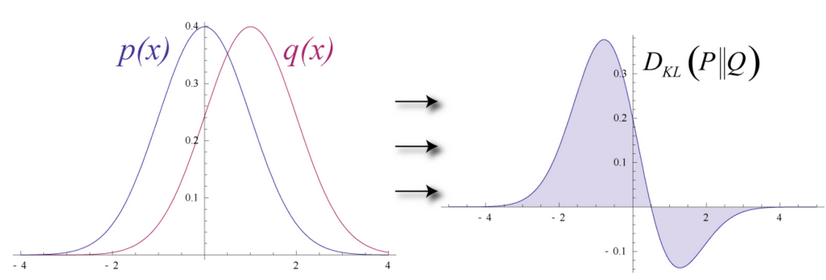
\includegraphics[width = 0.7\linewidth]{thesisfigures/KL_divergence_RBM.png}
 \caption{Illustration of the Kullback-Leibler divergence which measures the difference between two probability distributions $p(x)$ and $q(x)$.
 Figure taken from \href{https://deeplearning4j.org/restrictedboltzmannmachine}{here}.}
 \label{fig:KLdivergence}
\end{figure}



When the goal of the training is to approximate a probability distribution, as it is in generative modeling, another relevant measure is the \textbf{Kullback-Leibler divergence}, also known as the relative entropy or Shannon entropy (see figure \ref{fig:KLdivergence}). It is a non-symmetric measure of the dissimilarity between two probability density functions $p$ and $q$. If $p$ is the unkown probability which we approximate with $q$, we can measure the difference by
\begin{align}
	\text{KL}(p||q) = \int_{-\infty}^{\infty} p (\bm{x}) \log \frac{p(\bm{x})}{q(\bm{x})} \dif \bm{x}.
\end{align}
Thus, the Kullback-Leibler divergence between the distribution of the training data $f(\bm{x})$ and the model distribution $p(\bm{x}| \bm{\theta})$ is
\begin{align}
	\text{KL} (f(\bm{x})|| p(\bm{x}| \bm{\theta})) =& \int_{-\infty}^{\infty}
	f (\bm{x}) \log \frac{f(\bm{x})}{p(\bm{x}| \bm{\theta})} \dif \bm{x} \\
	=& \int_{-\infty}^{\infty} f(\bm{x}) \log f(\bm{x}) \dif \bm{x} - \int_{-\infty}^{\infty} f(\bm{x}) \log
	p(\bm{x}| \bm{\theta}) \dif \bm{x} \\
	%=& \mathbb{E}_{f(\bm{x})} (\log f(\bm{x})) - \mathbb{E}_{f(\bm{x})} (\log p(\bm{x}| \bm{\theta}))
	=& \langle \log f(\bm{x}) \rangle_{f(\bm{x})} - \langle \log p(\bm{x}| \bm{\theta}) \rangle_{f(\bm{x})} \\
	=& \langle \log f(\bm{x}) \rangle_{data} + \langle E(\bm{x}) \rangle_{data} + \log Z \\
	=& \langle \log f(\bm{x}) \rangle_{data} + \mathcal{C}_{LL} .
\end{align}
The first term is constant with respect to $\bm{\theta}$ since $f(\bm{x})$ is independent of $\bm{\theta}$. Thus the Kullback-Leibler Divergence is minimal when the second term is minimal. The second term is the log-likelihood cost function, hence minimizing the Kullback-Leibler divergence is equivalent to maximizing the log-likelihood.

To further understand generative models it is useful to study the gradient of the cost function which is needed in order to minimize it using methods presented in section \ref{sec:GD}. As in statistical physics the partition function is the generating function of expectation values, in particular there are mathematical relationships between expectation values and the log-partition function. In this case we have \cite{Mehta2018}

\begin{align}
	\langle \frac{ \partial E(\bm{x}; \theta_i) } { \partial \theta_i} \rangle_{model}
	= \int p(\bm{x}| \bm{\theta}) \frac{ \partial E(\bm{x}; \theta_i) } { \partial \theta_i} \dif \bm{x} 
	= -\frac{\partial \log Z(\theta_i)}{ \partial  \theta_i} .
\end{align}

Here $\langle \cdot \rangle_{model}$ is the expectation value over the model probability distribution $p(\bm{x}| \bm{\theta})$.
Using this relationship we can express the gradient of the cost function as
\begin{align}
	\frac{\partial \mathcal{C}_{LL}}{\partial \theta_i}
	=& \langle \frac{ \partial E(\bm{x}; \theta_i) } { \partial \theta_i} \rangle_{data} + \frac{\partial \log Z(\theta_i)}{ \partial  \theta_i} \\
	=& \langle \frac{ \partial E(\bm{x}; \theta_i) } { \partial \theta_i} \rangle_{data} - \langle \frac{ \partial E(\bm{x}; \theta_i) } { \partial \theta_i} \rangle_{model} \\
	%=& \langle O_i(\bm{x}) \rangle_{data} - \langle O_i(\bm{x}) \rangle_{model}
\end{align}
This expression shows that the gradient of the log-likelihood cost function is a \textbf{difference of moments}, with one calculated from the data and one calculated from the model. The data-dependent term is called the \textbf{positive phase} and the model-dependent term is called the \textbf{negative phase} of the gradient. We see now that minimizing the cost function results in lowering the energy of configurations $\bm{x}$ near points in the training data and increasing the energy of configurations not observed in the training data. That means we increase the model's probability of configurations similar to those in the training data.

The gradient of the cost function also demonstrates why gradients of unsupervised, generative models must be computed differently from for those of for example FNNs. While the data-dependent expectation value is easily calculated based on the samples $\bm{x}_i$ in the training data, we must sample from the model in order to generate samples from which to caclulate the model-dependent term. We sample from the model by using MCMC-based methods. We can not sample from the model directly because the partition function $Z$ is generally intractable.

As in supervised machine learning problems, the goal is also here to perform well on \textit{unseen} data, that is to have good generalization from the training data. The distribution $f(x)$ we approximate is not the \textit{true} distribution we wish to estimate, it is limited to the training data. Hence, in unsupervised training as well it is important to prevent overfitting to the training data. Thus it is common to add regularizers to the cost function in the same manner as described for the supervised methods.


\section{Gradient Descent Optimization}
\label{sec:GD}
Gradient descent is the most common method in machine learning for minimizing the cost function during the training stage. The goal is to iteratively update the parameters of the model in directions where the gradient of the cost function is large and negative. This procedure ensures that the parameters move towards a local minimum. In the simplest gradient descent scheme we start with initial parameter values  $\bm{\theta}_0$ and update according to
\begin{align}
	\mathbf{v}_t &= \eta_t \nabla_\theta \mathcal{C}(\bm{\theta}_t) \\
	\bm{\theta}_{t+1} &= \bm{\theta}_t - \mathbf{v}_t 	
\end{align}
where $\eta_t$ is a parameter which controls the step size and is called the \textbf{learning rate}.

To see the benefits and limitations to the gradient descent method we can compare it to Newton's method, which is  a \textit{second-order method}. In Newton's method the update $\bm{v}$ of the parameters is chosen in order to minimize the second-order Taylor expansion of the cost function:
\begin{align}
	\mathcal{C}(\bm{\theta} + \mathbf{v}) \approx \mathcal{C}(\bm{\theta}) + \nabla_\theta \mathcal{C}(\bm{\theta})\mathbf{v} + \frac{1}{2} \mathbf{v}^T H(\theta) \mathbf{v}
\end{align}
where $H(\theta)$ is the Hessian matrix of second derivatives. Differentiating this expression with respect to $\bm{v}$ and using that we should have $\nabla_\theta E(\bm{\theta} + \mathbf{v}_{opt}) = 0$ we find
\begin{align}
	0 = \nabla_\theta E(\bm{\theta}) + H(\theta) \mathbf{v}_{opt}
\end{align}
rewriting yields the update rules for Newton's method
\begin{align}
	\mathbf{v}_t &= H^{-1} (\theta_t) \nabla_\theta E(\theta_t) \\
	\bm{\theta}_{t+1} &= \bm{\theta}_t - \mathbf{v}_t
\end{align}
We cannot be sure that the Hessian is well conditioned so it is common to replace its inverse with a reregularized pseudo-inverse such as $[H(\theta_t)+\epsilon I ]^{-1}$, where $\epsilon$ is a small parameter. We see that Netwon's method has the same form as gradient descent, with the inverse Hessian acting as the learning rate. The benefit of this is that, while gradient descent has the same learning rate for all the parameters, in this case it is automatically adapted to each parameter individually, taking larger step in flat directions and smaller steps in steep directions. The reason is that the Hessian encodes the curvature of the surface, in the sense that its singular values are \textit{inversly proportional to the squares of the local curvatures of the surface}. However there are reasons why gradient descent is often preferred to second-order methods. It is an extremely intensive computational operation to calculate the Hessian. And even if one uses first-order methods to approximate the Hessian, known as quasi-Newton methods, one must still store and invert a matrix with $n^2$ entries, where $n$ is the number of parameters. \cite{Mehta2018}

The main consideration when choosing the gradient descent learning rate is a trade-off between accuracy and speed. While a small learning rate is guaranteed to converge to a local minimum, it may be very slow. A learning rate that is too big, on the other hand, can make the algorithm unstable, either oscillating around the minimum or even moving away from it, see fiugre \ref{fig:LearningRateMehta}. In the following sections we will look at some of the various improvements one can make to the simple gradient descent scheme.



\begin{figure}
\centering
 \includegraphics[width = 0.6\linewidth]{thesisfigures/LearningRateMehta.png}
 \caption{Effect of the learning rate $\eta$ on the gradient descent minimization algorithm.
 Taken from \href{https://deeplearning4j.org/restrictedboltzmannmachine}{here}.}
 \label{fig:LearningRateMehta}
\end{figure}




\subsection{Momentum}
One of the simplest modifications to the simple gradient descent algorithm is to introduce a term called \textbf{momentum}, which functions as a memory of the direction the algorithm is moving in parameter space. The update rule becomes
\begin{align}
		\mathbf{v}_t =& \gamma \mathbf{v}_{t-1} + \eta_t \nabla_\theta E(\bm{\theta}_t) \\
		\bm{\theta}_{t+1} =& \bm{\theta}_t - \mathbf{v}_t,
\end{align}
where $0 \leq \gamma \leq 1$ is the momentum hyperparameter, and $\mathbf{v}_t$ becomes a moving average over the most recent gradients with $(1-\gamma)^{-1}$ setting the characteristic time scale for the memory. Introducing momentum is useful because it increases the step size in directions with persistent but small gradients, and prevents oscillations in directions with high curvature.



\subsection{RMS-prop}
As mentioned, one ideally wants to adapt the learning rate to the curvature of the landscape without having to calculate the computationally expensive inverse of the Hessian matrix of second derivatives. Over the last years a number of algorithms have been developed which achieve this by keeping track of the second moment of the gradient in addition to the gradient itself. Some of these methods include AdaGrad, AdaDelta, RMS-prop, and ADAM. We will discuss RMS-prop and the ADAM optimizer. Multiplication and division by vectors is to be taken as element-wise operations.

The RMS-prop algorithm keeps track of the second moment of the gradient with the term $\mathbf{s}_t = \mathbb{E}[\mathbf{g}_t^2]$. The update rule is then given by
\begin{align}
	\mathbf{g}_t =& \nabla_\theta E(\bm{\theta}) \\
	\mathbf{s}_t =& \beta \mathbf{s}_{t-1} + (1-\beta)\mathbf{g}_t^2 \\
	\bm{\theta}_{t+1} =& \bm{\theta}_t - \eta_t \frac{\mathbf{g}_t}{\sqrt{\mathbf{s}_t + \epsilon}}.
\end{align}
Here $\beta$ sets the averaging time of the second moment and typically has a value around $\beta=0.9$. $\eta_t$ is the learning rate, typically $10^{-3}$, and $\epsilon \sim 10^{-8}$ is a regularization constant in order to prevent divergencies. As desired this update rule ensures that the learning rate is reduced in directions where the magnitude of the gradient is consistently large. We can therefore use a larger learning rate which speeds up the process.

\subsection{ADAM}
\label{sec:adam}
The ADAM optimizer keeps a moving average of both the first and second moment of the gradient, that is $\mathbf{m}_t = \mathbb{E}[\mathbf{g}_t]$ and $\mathbf{s}_t = \mathbb{E}[\mathbf{g}_t^2]$ respectively.
\begin{align}
	\mathbf{g}_t &= \nabla_\theta E(\bm{\theta}) \\
	\mathbf{m}_t &= \beta_1 \mathbf{m}_{t-1} + (1-\beta_1) \mathbf{g}_t \\
	\mathbf{s}_t &= \beta_2 \mathbf{s}_{t-1} + (1-\beta_2) \mathbf{g}_t^2 \\
	\hat{\mathbf{m}}_t &= \frac{\mathbf{m}_t}{1-\beta_1^t} \\
	\hat{\mathbf{s}}_t &= \frac{\mathbf{s}_t}{1-\beta_2^t} \\
	\bm{\theta}_{t+1} &= \bm{\theta}_t - \eta_t \frac{\hat{\mathbf{m}}_t}{\sqrt{\hat{\mathbf{s}}_t} + \epsilon}
\end{align}
Here the variables denoted by hats represent a bias correction introduced because we estimate the moments of the gradient using a moving average. $\eta$ and $\epsilon$ are the same as for RMS-prop and $\beta_1$ and $\beta_2$ control the memory lifetime of the first and second moment, typically taken as 0.9 and 0.99 respectively.

Like in RMS-prop the effective step size of a parameter depends on the magnitude of its gradient squared. 
We can investigate this further by looking at how a single parameter $\theta_t$ is updated in terms of the variance $\bf{\sigma}_t^2 = \hat{\mathbf{s}}_t  - (\hat{\mathbf{m}}_t)^2$. The update can be written
\begin{align}
	\Delta \theta_{t+1} = -\eta_t \frac{\hat{m}_t}{\sqrt{\sigma_t^2 + m_t^2} + \epsilon} .
\end{align}
If we consider the limits of this expression we see that
\begin{itemize}
	\item  If $\sigma_t^2 \ll  \hat{m}_t^2$ then  $\Delta \theta_{t+1} \rightarrow -\eta_t$. If the variance is small while the gradient is big, meaning we are moving persistently in steep directions, the maximum step size is limited to $\eta_t$.
	\item If  $\sigma^2 \gg \hat{m}_t^2$ then $\Delta \theta_{t+1} \rightarrow -\eta_t \hat{m}_t/ \sigma_t$. This means that if the variance is big, so that there are great fluctuations in the gradient, the learning rate becomes proportional to the mean of the gradients in units of the standard deviation. This is good because the standard deviation is a natural and adaptive scale for determining whether the gradient is large or small.
\end{itemize}
In conclusion, the ADAM optimizer is able to configure the learning rate to not become too big in steep directions, avoiding oscillations and divergencies, as well as being adaptive when the gradient is experiencing large fluctuations. 

While RMS-prop and ADAM allow for using a bigger learning rate which speeds up computations some have observed that these methods might not generalize as well. Generalization refers to whether the trained model preforms well on unseen test data after having been trained on the training data and is an important goal in machine learning. 











\chapter{The Restricted Boltzmann Machine}
\label{sec:RBMchapter}
%Put in RMF section?: Hopfield network if nodes deterministic rather than stochastic.
%Where discuss DBNs?

The restricted Boltzmann machine (RBM) is an unsupervised, generative neural network which became known when Hinton \textit{et al} presented an efficient algorithm for training it \cite{Hinton2002} and soon after used it as a building block in deep belief networks, which were introduced in a series of seminal papers that coined the term deep learning and reawakened interest in artificial neural networks \cite{Hinton2006a} \cite{Hinton2006} \cite{Hinton2007}.

This chapter gives an introduction to the restricted Boltzmann machine. First, the general Boltzmann machine, then the RBM and the original variant with binary visible and hidden units, the binary-binary RBM. Finally we will look at the variant used in this work, the Gaussian-binary RBM, as well as the RBM training procedure.





%This chapter gives an introduction to the unsupervised artificial neural network RBMs. First BM and RBM, then the original RBM with binary nodes, first used in quantum problems for spin-lattice models. Then, the GB which allows for continuous values and position QM.


%This is called a localist encoding, since only one hidden unit is used to generate the response vector. This is analogous to the hypothetical notion of grandmother cells in the brain, that are able to recognize only one kind of object. By contrast, an RBM uses a distributed encoding, where many units are involved in generating each output. Models that used vector-valued hidden variables, such as (PCA examples) also use distributed encodings. \cite{Murphy2012}



\section{The Boltzmann Machine}
\label{sec:BM}


\begin{figure}
\centering
 \includegraphics[width = 0.5\linewidth]{thesisfigures/BMwikipedia.png}
 \caption{The the Boltzmann machine represented by an undirected, graphical model. Blue nodes are hidden units and white nodes are visible units. The Boltzmann machine is a complete graph, meaning each pair of nodes is connected by an edge. The nodes are stochastic, which makes it a probabilistic graphical model. Figure from \href{https://en.wikipedia.org/wiki/Boltzmann_machine}{here}.}
 \label{fig:BMwikipedia}
\end{figure}


%Product of experts (Hinton 1999 article). MRF is a special case of PoEs. (a PoE model with exponential experts is an MRF with input variables x and latent variables h, which is expressed by the Hammersley and Clifford theorem.) Since we multiply the individual probabilities of the experts, it is obvious that we only get a high overall probability if all experts assign high individual probabilities. The PoE can therefore be interpreted as a council that judges a presented sample as being important if the judgement is unanimous. This stays in contrast to a mixture model [5] where the individual probabilities for a presented sample are summed up. Consequently, in a mixture model an expert or mixture can possibly overrule the others and the overall probability will only be low if all mixtures assign low proba- bility.
%\cite{Melchior2012}

%An RBM is a special case of a product of experts (PoE) (Hinton 1999), which is so-called because we are multiplying together a set of “experts” (here, potential functions on each edge) and then normalizing, whereas in a mixture of experts, we take a convex combination of normalized distributions. The intuitive reason why PoE models might work better than a mixture is that each expert can enforce a constraint (if the expert has a value which is $\gg$ 1 or $\ll$ 1) or a “don’t care” condition (if the expert has value 1). By multiplying these experts together in di erent ways we can create “sharp” distributions which predict data which satisfies the specified constraints (Hinton and Teh 2001). For example, consider a distributed model of text. A given document might have the topics “government”, “mafia” and “playboy”. If we “multiply” the predictions of each topic together, the model may give very high probability to the word “Berlusconi”9 (Salakhutdinov and Hinton 2010). By contrast, adding together experts can only make the distribution broader (see Figure 14.17).
%\cite{Murphy2012}

%While an MRF is a particular case of a PoE, a BM is an MRF with a particular energy function that leads to a complete undirected graph as shown in Figure 8.
%This implies a fully connected network where the pairwise communication between two units is symmetrical. The activation of each node is given by the sum over all values of its incoming connections. 


The Boltzmann machine \cite{Ackley1985} is a type of Markov Random Field (section \ref{sec:MRF}) where each pair of nodes is connected by an edge (see figure \ref{fig:BMwikipedia}). This means it is a fully connected network, or a \textbf{complete graph}. Furthermore the nodes are defined as either \textbf{visible} nodes, denoted by $\bm{x}$, or \textbf{hidden} nodes, denoted $\bm{h}$. The visible nodes are the input and output. The hidden nodes are latent variables of which the purpose is to encode complex interactions between the visible nodes. 

%Latent or hidden variables are a powerful yet elegant way to encode sophisticated correlations between observ- able features. The underlying reason for this is that marginalizing over a subset of variables – “integrating out” degrees of freedom in the language of physics – in- duces complex interactions between the remaining vari- ables. The idea that integrating out variables can lead to complex correlations is a familiar component of many physical theories. For example, when considering free electrons living on a lattice, integrating out phonons gives rise to higher-order electron-electron interactions (e.g. su- perconducting or magnetic correlations). More generally, in the Wilsonian renormalization group paradigm, all ef- fective field theories can be thought of as arising from integrating out high-energy degrees of freedom (Wilson and Kogut, 1974).
%Generative models with latent variables run this logic in reverse – encode complex interactions between visible variables by introducing additional, hidden variables that interact with visible degrees of freedom in a simple man- ner, yet still reproduce the complex correlations between visible degrees in the data once marginalized over (in- tegrated out). This allows us to encode complex higher- order interactions between the visible variables using sim- pler interactions at the cost of introducing new latent variables/degrees of freedom. This trick is also widely exploited in physics (e.g. in the Hubbard-Stratonovich transformation (Hubbard, 1959; Stratonovich, 1957) or the introduction of ghost fields in gauge theory (Faddeev and Popov, 1967)).

The joint probability density function of the variables is, similar to the MRF in equation \ref{eq:MRFhidden}, given by

\begin{align}
	p_{BM}(\bm{x}, \bm{h}) = \frac{1}{Z_{BM}} e^{-\frac{1}{T}E_{BM}(\bm{x}, \bm{h})} ,
\end{align}
with the partition function 
\begin{align}
	Z_{BM} = \int \int e^{-\frac{1}{T} E_{BM}(\tilde{\bm{x}}, \tilde{\bm{h}})} \dif \tilde{\bm{x}} \dif \tilde{\bm{h}} .
\end{align}

$T$ is a physics-inspired parameter named temperature and will be assumed to be 1 unless otherwise stated. The energy function of the Boltzmann machine determines the interactions between the nodes and is defined  

\begin{align}
	E_{BM}(\bm{x}, \bm{h}) =& - \sum_{i, k}^{M, K} a_i^k \alpha_i^k (x_i)
	- \sum_{j, l}^{N, L} b_j^l \beta_j^l (h_j) 
	- \sum_{i,j,k,l}^{M,N,K,L} \alpha_i^k (x_i) w_{ij}^{kl} \beta_j^l (h_j) \nonumber \\
	&- \sum_{i, m=i+1, k}^{M, M, K} \alpha_i^k (x_i) v_{im}^k \alpha_m^k (x_m)
	- \sum_{j,n=j+1,l}^{N,N,L} \beta_j^l (h_j) u_{jn}^l \beta_n^l (h_n).
\end{align}
Here $\alpha_i^k (x_i)$ and $\beta_j^l (h_j)$ are one-dimensional transfer functions or mappings from the given input value to the desired feature value. They can be arbitrary functions of the input variables and are independent of the parameterization (parameters referring to weight and biases), meaning they are not affected by training of the model. The indices $k$ and $l$ indicate that there can be multiple transfer functions per variable.
Furthermore, $a_i^k$ and $b_j^l$ are the visible and hidden bias. $w_{ij}^{kl}$ are weights of the \textbf{inter-layer} connection terms which connect visible and hidden units. $ v_{im}^k$ and $u_{jn}^l$ are weights of the \textbf{intra-layer} connection terms which connect the visible units to each other and the hidden units to each other, respectively.

\begin{comment}
\begin{itemize}
	\item $\alpha_i^k (x_i), \beta_j^l (h_j) $= One dimensional transfer functions, mapping a given input value to a desired feature value. They are sufficient statistics of the model and can be arbitrary non-parametrized functions of the input variable $x_i$ or $h_j$ respectively, but they need to be independent of the parametrization.
	\item $k, l $= These indices denote there can be multiple transfer funcs pr variable.
	\item $a_i^k,  b_j^l$= appear in the first and second term which only depends ont he visible and hidden units respectively. Thus they could be interpreted as the corresponding visible and hidden bias respectively.
	\item $w_{ij}^{kl}$ = inter layer connection term, connects the visible and hidden bias, respectively.
	\item $ v_{im}^k, u_{jn}^l$ = intra layer connection terms, connecting the visible units to each other, and the hidden units to each other, respectively.
\end{itemize}
\end{comment}

%This formalism allows to define even complexer BMs where more than two units interact with each other, named higher order BMs [36]. But a major disadvantage of BMs in general is that it is usually intractable to calculate the partition function since the integration over all possible states is only computable for small toy prob- lems.
%Therefore, training BMs is usually done by approximations using sampling methods [5], which will be described in detail later. So far it is just important to note that for those sampling methods we need to be able to calculate the conditional probability of the visible units given the hidden units and vice versa. Using Bayes theorem we can derive the conditional probability of the hidden units given the visible values and vice versa.



\subsection{Restricted Boltzmann Machines}
\label{sec:RBM}

\begin{figure}
\centering
 \includegraphics[width = 0.6\linewidth]{thesisfigures/RBMmehta.png}
 \caption{The bipartite graph structure of the restricted Boltzmann machine. In contrast to the general Boltzmann machine there are no connections within layers. Figure from \cite{Mehta2018}.}
 \label{fig:RBMmehta}
\end{figure}


The RBM was originally introduced in \cite{Smolensky1986} with the name \textbf{harmonium}, since the energy function was referred to as the \textit{harmony} at the time. It was introduced as the restricted Boltzmann machine by Hinton in \cite{Hinton2002}.
The RBM is a simpler version of the Boltzmann machine where there are no connections within layers. This means the units within the visible layer are conditionally independent of each other and the same for the units in the hidden layer. This makes the RBM a \textbf{bipartite} graph, see figure \ref{fig:RBMmehta}.

%A simplification where all lateral connections between visible units and all lateral connections between hidden units are removed, is a so called Restricted Boltzmann Machine (RBM). The RBMs structure is a bipartite graph where visible and hidden units are pairwise conditionally independent, shown in Figure 9.

%The major advantage of RBMs is that the units of the visible layer are conditional independent and so are the units of the hidden layer. This 

The conditional independency within layers leads to a factorization property of RBMs when marginalizing out the visible or hidden units. The integral over all possible states of the visible layer factorizes into a product of one
dimensional integrals over all possible values for the corresponding unit. Therefore, conditional probabilities can be computed efficiently. Having the conditional probabilities means Gibbs sampling, a simpler version of Metropolis-Hastings sampling, can be employed. 

\subsubsection{Energy Function}

We remove the intra-layer connections by setting $v_{im}$ and $u_{jn}$ to zero. The expression for the energy of the RBM is then
\begin{align}
	E_{RBM}(\bm{x}, \bm{h}) = - \sum_{i, k}^{M, K} a_i^k \alpha_i^k (x_i)
	- \sum_{j, l}^{N, L} b_j^l \beta_j^l (h_j) 
	- \sum_{i,j,k,l}^{M,N,K,L} \alpha_i^k (x_i) w_{ij}^{kl} \beta_j^l (h_j). \label{eq:RBMenergy}
\end{align}

%\subsubsection{Joint Probability Density Function}

\begin{comment}
\subsubsection{Marginal Probability Density Functions}
\begin{align}
	P_{RBM} (\bm{x}) =& \int P_{RBM} (\bm{x}, \tilde{\bm{h}}) \dif \tilde{\bm{h}} \nonumber \\
	=& \frac{1}{Z_{RBM}} \int e^{-E_{RBM} (\bm{x}, \tilde{\bm{h}}) } \dif \tilde{\bm{h}} \nonumber \\
	=& \frac{1}{Z_{RBM}} \int e^{\sum_{i, k} a_i^k \alpha_i^k (x_i)
	+ \sum_{j, l} b_j^l \beta_j^l (\tilde{h}_j) 
	+ \sum_{i,j,k,l} \alpha_i^k (x_i) w_{ij}^{kl} \beta_j^l (\tilde{h}_j)} 
	\dif \tilde{\bm{h}} \nonumber \\
	=& \frac{1}{Z_{RBM}} e^{\sum_{i, k} a_i^k \alpha_i^k (x_i)}
	\int \prod_j^N e^{\sum_l b_j^l \beta_j^l (\tilde{h}_j) 
	+ \sum_{i,k,l} \alpha_i^k (x_i) w_{ij}^{kl} \beta_j^l (\tilde{h}_j)} \dif \tilde{\bm{h}} \nonumber \\
	=& \frac{1}{Z_{RBM}} e^{\sum_{i, k} a_i^k \alpha_i^k (x_i)}
	\biggl( \int e^{\sum_l b_1^l \beta_1^l (\tilde{h}_1) + \sum_{i,k,l} \alpha_i^k (x_i) w_{i1}^{kl} \beta_1^l (\tilde{h}_1)} \dif  \tilde{h}_1 \nonumber \\
	& \times \int e^{\sum_l b_2^l \beta_2^l (\tilde{h}_2) + \sum_{i,k,l} \alpha_i^k (x_i) w_{i2}^{kl} \beta_2^l (\tilde{h}_2)} \dif  \tilde{h}_2 \nonumber \\
	& \times ... \nonumber \\
	& \times \int e^{\sum_l b_N^l \beta_N^l (\tilde{h}_N) + \sum_{i,k,l} \alpha_i^k (x_i) w_{iN}^{kl} \beta_N^l (\tilde{h}_N)} \dif  \tilde{h}_N \biggr) \nonumber \\
	=& \frac{1}{Z_{RBM}} e^{\sum_{i, k} a_i^k \alpha_i^k (x_i)}
	\prod_j^N \int e^{\sum_l b_j^l \beta_j^l (\tilde{h}_j) + \sum_{i,k,l} \alpha_i^k (x_i) w_{ij}^{kl} \beta_j^l (\tilde{h}_j)}  \dif \tilde{h}_j
\end{align}

Similarly
\begin{align}
	P_{RBM} (\bm{h}) =& \frac{1}{Z_{RBM}} \int e^{-E_{RBM} (\tilde{\bm{x}}, \bm{h})} \dif \tilde{\bm{x}} \nonumber \\
	=& \frac{1}{Z_{RBM}} e^{\sum_{j, l} b_j^l \beta_j^l (h_j)}
	\prod_i^M \int e^{\sum_k a_i^k \alpha_i^k (\tilde{x}_i)
	+ \sum_{j,k,l} \alpha_i^k (\tilde{x}_i) w_{ij}^{kl} \beta_j^l (h_j)} \dif \tilde{x}_i
\end{align}

\subsubsection{Conditional Probability Density Functions}
Using Bayes theorem:
\begin{align}
	P_{RBM} (\bm{h}|\bm{x}) =& \frac{P_{RBM} (\bm{x}, \bm{h})}{P_{RBM} (\bm{x})} \nonumber \\
	=& \frac{\frac{1}{Z_{RBM}} e^{\sum_{i, k} a_i^k \alpha_i^k (x_i)
	+ \sum_{j, l} b_j^l \beta_j^l (h_j) 
	+ \sum_{i,j,k,l} \alpha_i^k (x_i) w_{ij}^{kl} \beta_j^l (h_j)}}
	{\frac{1}{Z_{RBM}} e^{\sum_{i, k} a_i^k \alpha_i^k (x_i)}
	\prod_j^N \int e^{\sum_l b_j^l \beta_j^l (\tilde{h}_j) + \sum_{i,k,l} \alpha_i^k (x_i) w_{ij}^{kl} \beta_j^l (\tilde{h}_j)}  \dif \tilde{h}_j} \nonumber \\
	=& \prod_j^N \frac{e^{\sum_l b_j^l \beta_j^l (h_j) + \sum_{i,k,l} \alpha_i^k (x_i) w_{ij}^{kl} \beta_j^l (h_j)} }
	{\int e^{\sum_l b_j^l \beta_j^l (\tilde{h}_j) + \sum_{i,k,l} \alpha_i^k (x_i) w_{ij}^{kl} \beta_j^l (\tilde{h}_j)}  \dif \tilde{h}_j}
\end{align}
Similarly
\begin{align}
	P_{RBM} (\bm{x}|\bm{h}) =&  \frac{P_{RBM} (\bm{x}, \bm{h})}{P_{RBM} (\bm{h})} \nonumber \\
	=& \prod_i^M \frac{e^{\sum_k a_i^k \alpha_i^k (x_i)
	+ \sum_{j,k,l} \alpha_i^k (x_i) w_{ij}^{kl} \beta_j^l (h_j)}}
	{\int e^{\sum_k a_i^k \alpha_i^k (\tilde{x}_i)
	+ \sum_{j,k,l} \alpha_i^k (\tilde{x}_i) w_{ij}^{kl} \beta_j^l (h_j)} \dif \tilde{x}_i}
\end{align}
\end{comment}


\subsection{Binary-Binary Restricted Boltzmann Machines}
The original RBM had binary visible and hidden nodes. They were showned to be universal approximators of discrete distributions in \cite{LeRoux2008}. It was also shown that adding hidden units yields strictly improved modelling power. The common choice of binary values are 0 and 1. However, in some physics applications, -1 and 1 might be a more natural choice. We will here use 0 and 1.


\subsubsection{Energy Function}

\begin{table*}\centering
\ra{1.3}
\caption{This table shows how the terms in the restricted Boltzmann machine (RBM) energy function (equation \ref{eq:RBMenergy}) should be implemented in order to yield the binary-binary restricted boltzmann machine, that is an RBM where both visible and hidden units take binary values. }
\label{tab:BBrbm}
\begin{tabular}{lll}
\toprule
\toprule
Transfer functions & Biases & Weights \\ 
\midrule 
$\alpha_i^1 (x_i) = x_i$ & $a_i^1 = a_i$  & $w_{ij}^{11} = w_{ij}$ \\
$\beta_j^1 (h_j) = h_j$  & $b_j^1 = b_j$  &  \\
\bottomrule
\bottomrule
\end{tabular}
\end{table*}

Table \ref{tab:BBrbm} shows how the RBM energy function should be implemented for the binary-binary RBM, using only one transfer function, the identity, for each layer. This results in the energy

\begin{align}
	E_{BB}(\bm{x}, \mathbf{h}) = - \sum_i^M x_i a_i- \sum_j^N b_j h_j - \sum_{i,j}^{M,N} x_i w_{ij} h_j.
	\label{eq:BBenergy}
\end{align}


\subsubsection{Joint Probability Density Function}
With the energy given in equation \ref{eq:BBenergy}, the joint probability density function of the units in the binary-binary RBM becomes
\begin{align}
	p_{BB}(\bm{x}, \bm{h}) =& \frac{1}{Z_{BB}} e^{\sum_i^M a_i x_i + \sum_j^N b_j h_j + \sum_{ij}^{M,N} x_i w_{ij} h_j} \\
	=& \frac{1}{Z_{BB}} e^{\bm{x}^T \bm{a} + \bm{b}^T \bm{h} + \bm{x}^T \bm{W} \bm{h}}
\end{align}
with the partition function
\begin{align}
	Z_{BB} = \sum_{\bm{x}, \bm{h}} e^{\bm{x}^T \bm{a} + \bm{b}^T \bm{h} + \bm{x}^T \bm{W} \bm{h}} .
\end{align}

\subsubsection{Marginal Probability Density Functions}
In order to find the probability of any configuration of the visible units we derive the marginal probability density function.

\begin{align}
	p_{BB} (\bm{x}) =& \sum_{\bm{h}} p_{BB} (\bm{x}, \bm{h}) \\
	=& \frac{1}{Z_{BB}} \sum_{\bm{h}} e^{\bm{x}^T \bm{a} + \bm{b}^T \bm{h} + \bm{x}^T \bm{W} \bm{h}} \nonumber \\
	=& \frac{1}{Z_{BB}} e^{\bm{x}^T \bm{a}} \sum_{\bm{h}} e^{\sum_j^N (b_j + \bm{x}^T \bm{w}_{\ast j})h_j} \nonumber \\
	=& \frac{1}{Z_{BB}} e^{\bm{x}^T \bm{a}} \sum_{\bm{h}} \prod_j^N e^{ (b_j + \bm{x}^T \bm{w}_{\ast j})h_j} \nonumber \\
	=& \frac{1}{Z_{BB}} e^{\bm{x}^T \bm{a}} \bigg ( \sum_{h_1} e^{(b_1 + \bm{x}^T \bm{w}_{\ast 1})h_1}
	\times \sum_{h_2} e^{(b_2 + \bm{x}^T \bm{w}_{\ast 2})h_2} \times \nonumber \\
	& ... \times \sum_{h_2} e^{(b_N + \bm{x}^T \bm{w}_{\ast N})h_N} \bigg ) \nonumber \\
	=& \frac{1}{Z_{BB}} e^{\bm{x}^T \bm{a}} \prod_j^N \sum_{h_j} e^{(b_j + \bm{x}^T \bm{w}_{\ast j}) h_j} \nonumber \\
	=& \frac{1}{Z_{BB}} e^{\bm{x}^T \bm{a}} \prod_j^N (1 + e^{b_j + \bm{x}^T \bm{w}_{\ast j}}) .
\end{align}

A similar derivation yields the marginal probability of the hidden units

\begin{align}
	p_{BB} (\bm{h}) = \frac{1}{Z_{BB}} e^{\bm{b}^T \bm{h}} \prod_i^M (1 + e^{a_i + \bm{w}_{i\ast}^T \bm{h}}) .
\end{align}


\subsubsection{Conditional Probability Density Functions}
We derive the probability of the hidden units given the visible units using Bayes' rule:
\begin{align}
	p_{BB} (\bm{h}|\bm{x}) =& \frac{p_{BB} (\bm{x}, \bm{h})}{p_{BB} (\bm{x})} \nonumber \\
	=& \frac{ \frac{1}{Z_{BB}}  e^{\bm{x}^T \bm{a} + \bm{b}^T \bm{h} + \bm{x}^T \bm{W} \bm{h}} }
	        {\frac{1}{Z_{BB}} e^{\bm{x}^T \bm{a}} \prod_j^N (1 + e^{b_j + \bm{x}^T \bm{w}_{\ast j}})} \nonumber \\
	=& \frac{  e^{\bm{x}^T \bm{a}} e^{ \sum_j^N (b_j + \bm{x}^T \bm{w}_{\ast j} ) h_j} }
	        { e^{\bm{x}^T \bm{a}} \prod_j^N (1 + e^{b_j + \bm{x}^T \bm{w}_{\ast j}})} \nonumber \\
	=& \prod_j^N \frac{ e^{(b_j + \bm{x}^T \bm{w}_{\ast j} ) h_j}  }
	{1 + e^{b_j + \bm{x}^T \bm{w}_{\ast j}}} \nonumber \\
	=& \prod_j^N p_{BB} (h_j| \bm{x}) .
\end{align}
From this we find the probability of a hidden unit being "on" or "off":
\begin{align}
	p_{BB} (h_j=1 | \bm{x}) =&   \frac{ e^{(b_j + \bm{x}^T \bm{w}_{\ast j} ) h_j}  }
	{1 + e^{b_j + \bm{x}^T \bm{w}_{\ast j}}} \\
	=&  \frac{ e^{(b_j + \bm{x}^T \bm{w}_{\ast j} )}  }
	{1 + e^{b_j + \bm{x}^T \bm{w}_{\ast j}}} \\
	=&  \frac{ 1 }{1 + e^{-(b_j + \bm{x}^T \bm{w}_{\ast j})} } ,
\end{align}
and
\begin{align}
	p_{BB} (h_j=0 | \bm{x}) =\frac{ 1 }{1 + e^{b_j + \bm{x}^T \bm{w}_{\ast j}} } .
\end{align}

We see that the outcome is the sigmoid function, the same as is frequently used as non-linear activation functions in feedforward neural networks (figure \ref{fig:FNNactivationsMehta}).

%From Equation 27.101, we see that we activate hidden node k in proportion to how much the input vector v “looks like” the weight vector w:,k (up to scaling factors). Thus each hidden node captures certain features of the input, as encoded in its weight vector, similar to a feedforward neural network. \cite{Murphy}

Similarly we have that the conditional probability of the visible units given the hidden are
\begin{align}
	p_{BB} (\bm{x}|\bm{h}) =& \prod_i^M \frac{ e^{ (a_i + \bm{w}_{i\ast}^T \bm{h}) x_i} }{ 1 + e^{a_i + \bm{w}_{i\ast}^T \bm{h}} } \\
	&= \prod_i^M p_{BB} (x_i | \bm{h}) .
\end{align}
Thus
\begin{align}
	p_{BB} (x_i=1 | \bm{h}) =& \frac{1}{1 + e^{-(a_i + \bm{w}_{i\ast}^T \bm{h} )}} \\
	p_{BB} (x_i=0 | \bm{h}) =& \frac{1}{1 + e^{a_i + \bm{w}_{i\ast}^T \bm{h} }} .
\end{align}






\subsection{Gaussian-Binary Restricted Boltzmann Machines}
%Other types of units: In the original definition of BMs [2], the visible and hidden units have binary values. However, in most cases the input data is coming from a continuous rather than a binary domain. Therefore, it would be of most interest to have the opportunity to choose continuous units as well. An easy way, making the original BM handle continuous data is simply to rescale the data into the interval [0, 1] and considering it as the probability for the corresponding unit taking the value one. However, the model is still assuming an underlying binary representation, so that this variant usually works not very well. If we assume the data coming truly from the interval $[0, \infty)$ the conditional prob- abilities (97) become exponential densities. This causes the normalization constant not to exist in each case so that truncated exponentials over the interval [0,1] are used instead, which leads to the so called Truncated Exponential RBMs [15] A natural assumption when dealing with continuous variables is assuming them to be Gaussian distributed and therefore, a distribution over R . This leads to the so called Gaussian-Binary RBM, which has been used successfully to model continuous domains and will be discussed in the next chapter. So far we considered only the visible layer to have continuous values but one can also think of RBMs with continuous visible and hidden layer like a Gaussian-Gaussian RBM for example. But as we will see, training an RBM with continuous visible and binary hidden layer tends to be difficult already. Furthermore this training issue be- comes crucial when having only continuous units since they get much more effected to sampling noise. This makes them uninteresting in practice although a completely continuous network seems to be the more powerful configuration. \cite{Melchior2012}

% Also discussion in Learning a Generative Model of Images by Factoring Appearance and Shape
In a number of problems the values we want to model are not binary, but continuous. There are several ways one might accomodate this. One way is the Gaussian-binary RBM \cite{Welling2005}. In this model the hidden units are still binary, while the visible units are assumed to take real values $x_i \in [-\infty, \infty]$ and be normally distributed with variance $\sigma_i^2$. 

\subsubsection{Energy Function}



\begin{table*}\centering
\ra{1.3}
\caption{This table shows how the terms in the restricted Boltzmann machine (RBM) energy function (equation \ref{eq:RBMenergy}) should be implemented in order to yield the Gaussian-binary restricted boltzmann machine, that is an RBM where the visible units take continuous values and the hidden units take binary values.}
\label{tab:GBrbm}
\begin{tabular}{lll}
\toprule
\toprule
Transfer functions & Biases & Weights \\ 
\midrule 
$\alpha_i^1 (x_i) = -x_i^2$  & $a_i^1 = \frac{1}{2\sigma_i^2}$      & $w_{ij}^{11} = 0$ \\
$\alpha_i^2 (x_i) = x_i$     & $a_i^2 = \frac{a_i}{\sigma_i^2}$     & $w_{ij}^{21} = \frac{w_{ij}}{\sigma_i^2}$ \\
$\alpha_i^3 (x_i) = 1$       & $a_i^3 = -\frac{a_i^2}{2\sigma_i^2}$ & $w_{ij}^{31} = 0$ \\
$\beta_j^1 (h_j) = h_j$      & $b_j^1 = b_j$                        &  \\
\bottomrule
\bottomrule
\end{tabular}
\end{table*}

We find the energy function of the Gaussian-binary RBM by implementing the RBM energy as shown in table \ref{tab:GBrbm}. As seen there are now three transfer functions for the visible units ($K=3$) and one for the hidden units ($L=1$).
Inserting into the expression for $E_{RBM}(\bm{x},\bm{h})$ in equation \ref{eq:RBMenergy} results in the energy
\begin{align}
	E_{GB}(\bm{x}, \bm{h}) =& \sum_i^M \frac{(x_i - a_i)^2}{2\sigma_i^2}
	- \sum_j^N b_j h_j 
	-\sum_{ij}^{M,N} \frac{x_i w_{ij} h_j}{\sigma_i^2} \nonumber \\
	=& \norm*{\frac{\bm{x} -\bm{a}}{2\bm{\sigma}}}^2 - \bm{b}^T \bm{h} 
	- (\frac{\bm{x}}{\bm{\sigma}^2})^T \bm{W}\bm{h} . \label{eq:GBenergy}
\end{align}

%adress sigma squared or not.

\subsubsection{Joint Probability Density Function}
Given the energy in equation \ref{eq:GBenergy}, joint probability density function of the Gaussian-binary RBM is
\begin{align}
	p_{GB} (\bm{x}, \bm{h}) =& \frac{1}{Z_{GB}} e^{-\norm*{\frac{\bm{x} -\bm{a}}{2\bm{\sigma}}}^2 + \bm{b}^T \bm{h} 
	+ (\frac{\bm{x}}{\bm{\sigma}^2})^T \bm{W}\bm{h}} \nonumber \\
	=& \frac{1}{Z_{GB}} e^{- \sum_i^M \frac{(x_i - a_i)^2}{2\sigma_i^2}
	+ \sum_j^N b_j h_j 
	+\sum_{ij}^{M,N} \frac{x_i w_{ij} h_j}{\sigma_i^2}} \nonumber \\
	=& \frac{1}{Z_{GB}} \prod_{ij}^{M,N} e^{-\frac{(x_i - a_i)^2}{2\sigma_i^2}
	+ b_j h_j 
	+\frac{x_i w_{ij} h_j}{\sigma_i^2}} ,
\end{align}
%=& \frac{1}{Z_{GB}} \prod_{ij}^{M,N} \phi_{GB_{ij}} (x_i, h_j) ,

with the partition function given by
\begin{align}
	Z_{GB} =& \int \sum_{\tilde{\bm{h}}}^{\tilde{\bm{H}}} e^{-\norm*{\frac{\tilde{\bm{x}} -\bm{a}}{2\bm{\sigma}}}^2 + \bm{b}^T \tilde{\bm{h}} 
	+ (\frac{\tilde{\bm{x}}}{\bm{\sigma}^2})^T \bm{W}\tilde{\bm{h}}} \dif \tilde{\bm{x}} .
\end{align}
%=& \int \sum_{\tilde{\bm{h}}}^{\tilde{\bm{H}}} \prod_{ij}^{M, N} \phi_{GB_{ij}} (\tilde{x}_i, \tilde{h}_j) \dif \tilde{\bm{x}} .

\subsubsection{Marginal Probability Density Functions}
We proceed to find the marginal probability densitites of the Gaussian-binary RBM. We first marginalize over the binary hidden units to find $p_{GB} (\bm{x})$

\begin{align}
	p_{GB} (\bm{x}) =& \sum_{\tilde{\bm{h}}}^{\tilde{\bm{H}}} p_{GB} (\bm{x}, \tilde{\bm{h}}) \nonumber \\
	=& \frac{1}{Z_{GB}} \sum_{\tilde{\bm{h}}}^{\tilde{\bm{H}}} 
	e^{-\norm*{\frac{\bm{x} -\bm{a}}{2\bm{\sigma}}}^2 + \bm{b}^T \tilde{\bm{h}} 
	+ (\frac{\bm{x}}{\bm{\sigma}^2})^T \bm{W}\tilde{\bm{h}}} \nonumber \\
	=& \frac{1}{Z_{GB}} e^{-\norm*{\frac{\bm{x} -\bm{a}}{2\bm{\sigma}}}^2}
	\prod_j^N (1 + e^{b_j + (\frac{\bm{x}}{\bm{\sigma}^2})^T \bm{w}_{\ast j}} ) .
\end{align}

We next marginalize over the visible units. This is the first time we marginalize over continuous values. We rewrite the exponential factor dependent on $\bm{x}$ as a Gaussian function before we integrate in the last step.

\begin{align}
	p_{GB} (\bm{h}) =& \int p_{GB} (\tilde{\bm{x}}, \bm{h}) \dif \tilde{\bm{x}} \nonumber \\
	=& \frac{1}{Z_{GB}} \int e^{-\norm*{\frac{\tilde{\bm{x}} -\bm{a}}{2\bm{\sigma}}}^2 + \bm{b}^T \bm{h} 
	+ (\frac{\tilde{\bm{x}}}{\bm{\sigma}^2})^T \bm{W}\bm{h}} \dif \tilde{\bm{x}} \nonumber \\
	=& \frac{1}{Z_{GB}} e^{\bm{b}^T \bm{h} } \int \prod_i^M
	e^{- \frac{(\tilde{x}_i - a_i)^2}{2\sigma_i^2} + \frac{\tilde{x}_i \bm{w}_{i\ast}^T \bm{h}}{\sigma_i^2} } \dif \tilde{\bm{x}} \nonumber \\
	=& \frac{1}{Z_{GB}} e^{\bm{b}^T \bm{h} }
	\biggl( \int e^{- \frac{(\tilde{x}_1 - a_1)^2}{2\sigma_1^2} + \frac{\tilde{x}_1 \bm{w}_{1\ast}^T \bm{h}}{\sigma_1^2} } \dif \tilde{x}_1 \nonumber \\
	& \times \int e^{- \frac{(\tilde{x}_2 - a_2)^2}{2\sigma_2^2} + \frac{\tilde{x}_2 \bm{w}_{2\ast}^T \bm{h}}{\sigma_2^2} } \dif \tilde{x}_2 \nonumber \\
	& \times ... \nonumber \\
	&\times \int e^{- \frac{(\tilde{x}_M - a_M)^2}{2\sigma_M^2} + \frac{\tilde{x}_M \bm{w}_{M\ast}^T \bm{h}}{\sigma_M^2} } \dif \tilde{x}_M \biggr) \nonumber \\
	=& \frac{1}{Z_{GB}} e^{\bm{b}^T \bm{h}} \prod_i^M
	\int e^{- \frac{(\tilde{x}_i - a_i)^2 - 2\tilde{x}_i \bm{w}_{i\ast}^T \bm{h}}{2\sigma_i^2} } \dif \tilde{x}_i \nonumber \\
	=& \frac{1}{Z_{GB}} e^{\bm{b}^T \bm{h}} \prod_i^M
	\int e^{- \frac{\tilde{x}_i^2 - 2\tilde{x}_i(a_i + \tilde{x}_i \bm{w}_{i\ast}^T \bm{h}) + a_i^2}{2\sigma_i^2} } \dif \tilde{x}_i \nonumber \\
	=& \frac{1}{Z_{GB}} e^{\bm{b}^T \bm{h}} \prod_i^M
	\int e^{- \frac{\tilde{x}_i^2 - 2\tilde{x}_i(a_i + \bm{w}_{i\ast}^T \bm{h}) + (a_i + \bm{w}_{i\ast}^T \bm{h})^2 - (a_i + \bm{w}_{i\ast}^T \bm{h})^2 + a_i^2}{2\sigma_i^2} } \dif \tilde{x}_i \nonumber \\
	=& \frac{1}{Z_{GB}} e^{\bm{b}^T \bm{h}} \prod_i^M
	\int e^{- \frac{(\tilde{x}_i - (a_i + \bm{w}_{i\ast}^T \bm{h}))^2 - a_i^2 -2a_i \bm{w}_{i\ast}^T \bm{h} - (\bm{w}_{i\ast}^T \bm{h})^2 + a_i^2}{2\sigma_i^2} } \dif \tilde{x}_i \nonumber \\
	=& \frac{1}{Z_{GB}} e^{\bm{b}^T \bm{h}} \prod_i^M
	e^{\frac{2a_i \bm{w}_{i\ast}^T \bm{h} +(\bm{w}_{i\ast}^T \bm{h})^2 }{2\sigma_i^2}}
	\int e^{- \frac{(\tilde{x}_i - a_i - \bm{w}_{i\ast}^T \bm{h})^2}{2\sigma_i^2}}
	\dif \tilde{x}_i \nonumber \\
	=& \frac{1}{Z_{GB}} e^{\bm{b}^T \bm{h}} \prod_i^M
	\sqrt{2\pi \sigma_i^2}
	e^{\frac{2a_i \bm{w}_{i\ast}^T \bm{h} +(\bm{w}_{i\ast}^T \bm{h})^2 }{2\sigma_i^2}} .
\end{align}
%Used the physics latent variable transformation trick.
%Thus we can calculate the partition function, using factorization..?

\subsubsection{Conditional Probability Density Functions}
We finish by deriving the conditional probabilities. 
\begin{align}
	p_{GB} (\bm{h}| \bm{x}) =& \frac{p_{GB} (\bm{x}, \bm{h})}{p_{GB} (\bm{x})} \nonumber \\
	=& \frac{\frac{1}{Z_{GB}} e^{-\norm*{\frac{\bm{x} -\bm{a}}{2\bm{\sigma}}}^2 + \bm{b}^T \bm{h} 
	+ (\frac{\bm{x}}{\bm{\sigma}^2})^T \bm{W}\bm{h}}}
	{\frac{1}{Z_{GB}} e^{-\norm*{\frac{\bm{x} -\bm{a}}{2\bm{\sigma}}}^2}
	\prod_j^N (1 + e^{b_j + (\frac{\bm{x}}{\bm{\sigma}^2})^T \bm{w}_{\ast j}} ) }
	\nonumber \\
	=& \prod_j^N \frac{e^{(b_j + (\frac{\bm{x}}{\bm{\sigma}^2})^T \bm{w}_{\ast j})h_j } }
	{1 + e^{b_j + (\frac{\bm{x}}{\bm{\sigma}^2})^T \bm{w}_{\ast j}}} \nonumber \\
	=& \prod_j^N p_{GB} (h_j|\bm{x})
\end{align}

The conditional probability of a binary hidden unit $h_j$ being on or off again take the form of sigmoid functions
\begin{align}
	p_{GB} (h_j =1 | \bm{x}) =& \frac{e^{b_j + (\frac{\bm{x}}{\bm{\sigma}^2})^T \bm{w}_{\ast j} } }
	{1 + e^{b_j + (\frac{\bm{x}}{\bm{\sigma}^2})^T \bm{w}_{\ast j}}} \nonumber \\
	=& \frac{1}{1 + e^{-b_j - (\frac{\bm{x}}{\bm{\sigma}^2})^T \bm{w}_{\ast j}}} \\
	p_{GB} (h_j =0 | \bm{x}) =&
	\frac{1}{1 + e^{b_j +(\frac{\bm{x}}{\bm{\sigma}^2})^T \bm{w}_{\ast j}}} .
\end{align}

The conditional probability of the continuous $\bm{x}$ now has another form, however.
\begin{align}
	p_{GB} (\bm{x}|\bm{h})
	=& \frac{p_{GB} (\bm{x}, \bm{h})}{p_{GB} (\bm{h})} \nonumber \\
	=& \frac{\frac{1}{Z_{GB}} e^{-\norm*{\frac{\bm{x} -\bm{a}}{2\bm{\sigma}}}^2 + \bm{b}^T \bm{h} 
	+ (\frac{\bm{x}}{\bm{\sigma}^2})^T \bm{W}\bm{h}}}
	{\frac{1}{Z_{GB}} e^{\bm{b}^T \bm{h}} \prod_i^M
	\sqrt{2\pi \sigma_i^2}
	e^{\frac{2a_i \bm{w}_{i\ast}^T \bm{h} +(\bm{w}_{i\ast}^T \bm{h})^2 }{2\sigma_i^2}}}
	\nonumber \\
	=& \prod_i^M \frac{1}{\sqrt{2\pi \sigma_i^2}}
	\frac{e^{- \frac{(x_i - a_i)^2}{2\sigma_i^2} + \frac{x_i \bm{w}_{i\ast}^T \bm{h}}{2\sigma_i^2} }}
	{e^{\frac{2a_i \bm{w}_{i\ast}^T \bm{h} +(\bm{w}_{i\ast}^T \bm{h})^2 }{2\sigma_i^2}}}
	\nonumber \\
	=& \prod_i^M \frac{1}{\sqrt{2\pi \sigma_i^2}}
	\frac{e^{-\frac{x_i^2 - 2a_i x_i + a_i^2 - 2x_i \bm{w}_{i\ast}^T\bm{h} }{2\sigma_i^2} } }
	{e^{\frac{2a_i \bm{w}_{i\ast}^T \bm{h} +(\bm{w}_{i\ast}^T \bm{h})^2 }{2\sigma_i^2}}}
	\nonumber \\
	=& \prod_i^M \frac{1}{\sqrt{2\pi \sigma_i^2}}
	e^{- \frac{x_i^2 - 2a_i x_i + a_i^2 - 2x_i \bm{w}_{i\ast}^T\bm{h}
	+ 2a_i \bm{w}_{i\ast}^T \bm{h} +(\bm{w}_{i\ast}^T \bm{h})^2}
	{2\sigma_i^2} }
	\nonumber \\
	=& \prod_i^M \frac{1}{\sqrt{2\pi \sigma_i^2}}
	e^{ - \frac{(x_i - b_i - \bm{w}_{i\ast}^T \bm{h})^2}{2\sigma_i^2}} \nonumber \\
	=& \prod_i^M \mathcal{N}
	(x_i | b_i + \bm{w}_{i\ast}^T \bm{h}, \sigma_i^2) \\
	\Rightarrow p_{GB} (x_i|\bm{h}) =& \mathcal{N}
	(x_i | b_i + \bm{w}_{i\ast}^T \bm{h}, \sigma_i^2) .
\end{align}

The form of these conditional probabilities explain the name "Gaussian" and the form of the Gaussian-binary energy function. We see that the conditional probability of $x_i$ given $\bm{h}$ is a normal distribution with mean $b_i + \bm{w}_{i\ast}^T \bm{h}$ and variance $\sigma_i^2$.

\begin{comment}
\subsubsection{Further analysis of the GB-RBM - the marginal prob as a MoG}

\subsection{Gaussian-something continuous RBM?}
If we use Gaussian latent variables and Gaussian visible variables, we get an undirected version of factor analysis. However, it turns out that it is identical to the standard directed version (Marks and Movellan 2001).
If we use Gaussian latent variables and categorical observed variables, we get an undirected version of categorical PCA (Section 27.2.2). In (Salakhutdinov et al. 2007), this was applied to the Netflix collaborative filtering problem, but was found to be significantly inferior to using binary latent variables, which have more expressive power. \cite{Murphy2012}
\end{comment}




\section{Training the RBM}

The cost function of the RBM is most commonly chosen to be the negative log-likelihood and will have a similar form as discussed in \ref{sec:UnsupervisedCostfunction}. It is usually minimized using gradient descent algorithms like those discussed in \ref{sec:GD}. The one thing we will explain here however is the Gibbs sampling used to compute the gradient of the log likelihood cost function. In order to compute the gradient we need to sample configurations $\bm{x}$ from the model. This is done using MCMC methods. Since we usually know the conditional probabilities we can use a special case of Metropolis-Hastings called Gibbs sampling.

\subsection{Gibbs Sampling}
The Gibbs sampling method use the same framework as the Metropolis-Hastings algorithm (section \ref{sec:MetroHastings}) employing Markov Chains and Monte Carlo sampling. The only difference lies in how the update step is implemented. 
Recall that the Metropolis Hastings acceptance step is
\begin{align}
	A(\bm{x}^f, \bm{x}^b) = \text{min} \Big(1,  \frac{  P(\bm{x}^f) Q(\bm{x}^b| \bm{x}^f) }
	{  P(\bm{x}^b) Q(\bm{x}^f| \bm{x}^b)  }  \Big)
\end{align}

where the before and final states are denoted by $b$ and $f$ respectively and these are made superscripts in order to easily index the vector components with subscripts.

Gibbs sampling offer a smart way of choosing the proposal distribution depending on the desired distribution. Given the desired distribution $p(\bm{x}) = p(x_1, ...x_D)$ we need to formulate the proposal distribution as the conditional probability of a variable $x_i$ given all the other variables $\bm{x}_{\setminus i} = \{ x_1, ..., x_D \} \setminus \{x_i\}$.
The proposal distribution is then given by $p(x_i | \bm{x}_{\setminus i})$ and we can use it to express the desired distribution by $p(\bm{x}) = p(x_i | \bm{x}_{\setminus i}) p(\bm{x}_{\setminus i})$ . We then insert this into the Metropolis-Hastings acceptance probability. 

\begin{align}
	A(\bm{x}^f, \bm{x}^b) =& \text{min} \Big(1,  \frac{  P(\bm{x}^f) Q(\bm{x}^b| \bm{x}^f) }
	{  P(\bm{x}^b) Q(\bm{x}^f| \bm{x}^b)  }  \Big) \\
	=& \text{min} \Big(1,  \frac{  P(\bm{x}^f) P(x_i^b| \bm{x}_{\setminus i}^f) }
	{  P(\bm{x}^b) P(x_i^f| \bm{x}_{\setminus i}^b)  }  \Big) \\
	=& \text{min} \Big(1,  \frac{ P(x_i^f| \bm{x}_{\setminus i}^f)  P(\bm{x}_{\setminus i}^f) P(x_i^b| \bm{x}_{\setminus i}^f) }
	{   P(x_i^b| \bm{x}_{\setminus i}^b) P(\bm{x}_{\setminus i}^b) P(x_i^f| \bm{x}_{\setminus i}^b)  }  \Big) \\
	=& \text{min} \Big(1,  \frac{ P(x_i^f| \bm{x}_{\setminus i}^b)  P(\bm{x}_{\setminus i}^b) P(x_i^b| \bm{x}_{\setminus i}^b) }
	{   P(x_i^b| \bm{x}_{\setminus i}^b) P(\bm{x}_{\setminus i}^b) P(x_i^f| \bm{x}_{\setminus i}^b)  }  \Big) \\ \label{eq:GibbsAlgebra}
	=& 1,
\end{align}
where in \ref{eq:GibbsAlgebra} we used that only $\bm{x}_i^b$ is updated to $\bm{x}_i^f$ and so $\bm{x}_{\setminus i}^f = \bm{x}_{\setminus i}^b$. It turns out that the ratio becomes one, which means all samples are accepted in Gibbs sampling.

In the RBM the visible units are conditionally independent of each other and it is the same for the hidden units. The proposal distribution is therefore
\begin{align}
	Q(x_i | \bm{x}_{\setminus i}^b, \bm{h}) =& p_{RBM} (x_i |\bm{h}) \\
	Q(h_j | \bm{x}, \bm{h}_{\setminus j}^b) =& p_{RBM} (h_j |\bm{x}). 
\end{align}



\begin{comment}
\subsection{Notes from publications (not section in the final thesis)}

\begin{itemize}
	\item \textbf{Summary from}
	\begin{itemize}
		\item \textbf{2017: Wang, Melchior, Wiskott: Gaussian-binary Restricted Boltzmann Machines on Modeling Natural Image Statistics} \cite{Melchior2017}
\end{itemize}
	\item First proposed by
	\begin{itemize}
		\item 2005 Welling, Rosen-Zvi, Hinton: Exponential Family Harmoniums with an Application to Information Retrieval \cite{Welling2005}
	\end{itemize}
	\item A common choice når man trenger cont visibles, ref
	\begin{itemize}
		\item 2009 A. Krizhevsky: Learning multiple layers of features from tiny images (master's thesis) \cite{Krizhevsky2009}
		\item 2011 Cho, Ilin, Raiko: Improved learning of gaussian-bernoulli restricted boltzmann machines \cite{Cho2011}
	\end{itemize}
	\item Training known to be hard, modifiactions to improve it proposed by:
	\begin{itemize}
		\item 2007 Lee, Ekanadham, Ng: Used a sparse penalty during training, allowing them to learn meaningful features from natural image patches (Sparse deep belief net model for visual area v2) \cite{Lee2008}
		\item 2009 A. Krizhevsky: Trained GRBMs on natural images and concluded the difficulties are mainly due to the existence of high-frequency noise in the images, which further prevents the model from learning the important structures. (referenced above) \cite{Krizhevsky2009}
		\item 2011 Theis, Gerwinn, Sinz, Bethge: Illustrates that in terms of likelihood estimation GRBMs are already outperformed by simple mixture models. (In all likelihood, deep belief is not enough) \cite{Theis2011}
		\item Focus on improving the model in the view of generative models
		\begin{itemize}
			\item 2010 Ranzato, Krizhevsky, Hinton: Factored 3-way restricted boltzmann machines for modeling natural images \cite{Ranzato2010}
			\item 2010 Ranzato, Hinton: Modeling pixel means and covariances using factorized third-order boltzmann machines \cite{Ranzato2010a}
			\item 2011 Courville, Bergstra, Bengio: A spike and slab restricted boltzmann machine \cite{Courville2011}
			\item 2011 Le Roux, Heess, Shotton, Winn: Learning a generative model of images by factoring appearance and shape \cite{LeRoux2011}
		\end{itemize}
		\item 2011 Cho, Ilin, Raiko: Suggested the failure of GRBMs is due to the training algo and proposed some modifications to overcome the difficulties encountered in training GRBMs (referenced above) \cite{Cho2011}
	\end{itemize}
	\item All these studies have shown the failures of GRBMs empirically, but to our knowledge there is no analysis of GRBMs apart from out preliminary work:
	\begin{itemize}
		\item 2012 Wang, Melchior, Wiskott: (An analysis of gaussian-binary boltzmann machines for natural image) \cite{Wang2012}
	\end{itemize}
	which accounts the reasons behind these failiures. In this paper, we extend our work in which we consider GRBMs from the perspective of density models, i.e. how well the model learns the dist of the data.
	\item We show an GB-RBM can be regarded as a mixture of Gaussians, which has already been mentioned briefly in previous studies:
	\begin{itemize}
		\item 2009 Bengio: Learning deep architectures for AI \cite{Bengio2009}
		\item 2011 Theis, Gerwinn, Sinz, Bethge: referenced above \cite{Theis2011}
		\item 2011 Courville, Bergstra, Bengio: referenced above \cite{Courville2011}
	\end{itemize}
	but has gone unheeded. This formulation makes clear that GRBMs are quite limited in the way they can represent data. However we argue this fact does not necessarily prevent the model from learning the statistical structure in the data. 
	\item We present successful training of GRBMs both on a two-dimensional blind source separation problem and natural image patches, and that the results are comparable to that of independent component analysis (ICA). 
	\item Based on our analysis we propose several training recipes, which allowed successful and fast training in our experiments. 
	\item Finally, we discuss the relationship between GRBMs and above mentioned modifications of the model.
\end{itemize}


\begin{itemize}
	\item \textbf{Summary from}
	\begin{itemize}
		\item \textbf{2012 Melchoir: Learning natural image statistics with gaussian-binary restricted boltzmann machines (Master's thesis)} \cite{Melchior2012}
\end{itemize}
	\item A popular variant of RBM is GB-RBM
	\begin{itemize}
		\item 2004 Welling, Rosen-Zvi, Hinton: \cite{Welling2005} referenced above
	\end{itemize}
	\item Training difficulties
	\begin{itemize}
		\item 2010 Fischer, Igel: RBMs difficult to train (Markov-random-fields und boltzmann maschinen)
		\item 2012 Wang, Melchior, Wiskott: This even more critical when using GB-RBMs (referenced above) \cite{Wang2012}
	\end{itemize}
	Several modifications proposed to overcome training difficulties
	\begin{itemize}
		\item 2007 Lee, Ekanadham, Ng: Added a sparseness penalty on the gradient that forced the model to prefer sparse representations and seems to help learning meaningful features (referenced above) \cite{Lee2008}
		\item 2011 Cho, Ilin, Raiko: Suggested the training failure is due to the training algo and proposed several improvements to overcome the problem (referenced above) \cite{Cho2011}
		\item 2009 A. Krizhevsky: Successfully trained a deep hierarchical network and concluded that a failure is mainly because of the existence of high-frequency noise in natural images, which prevents the model from learning the important structures. (referenced above) \cite{Krizhevsky2009}
		\item Other approaches modified the model such that it is capable of modelling higher order statistics directly:
		\begin{itemize}
			\item 2011 Courville, Bergstra, Bengio: referenced above \cite{Courville2011}
			\item 2010 Ranzato, Hinton: referenced above \cite{Ranzato2010a}
			\item 2010 Ranzato, Krizhevsky, Hinton: referenced above \cite{Ranzato2010}
		\end{itemize}
		All modifications showed that BG-RBMs are in principle capable of learning features comparable to the receptive fields in the early primary visual cortex V1, but in practice this is difficult to achieve.
		\item To derive a better understanding of the limitations of the model, the authors in
		\begin{itemize}
			\item 2011 Le Roux, Heess, Shotton, Winn: ref above \cite{LeRoux2011}
		\end{itemize} 
		evaluated its capabilities from the perspective of image reconstruction. In
		\begin{itemize}
			\item 2011 Theis, Gerwinn, Sinz, Bethge: ref above \cite{Theis2011}
		\end{itemize} 
		the likelihood of the model is compared to classical machine learning methods. Although the model has been analysed to show the failures empirically, there are few works accounting for the failure analytically.
	\end{itemize}
	\item Other interesting points made:
	\begin{itemize}
		\item 1986 Hinton, Sejnowski: The Boltzmann machine (Learning and relearning in boltzmann machines) \cite{Hinton1986}
		\item 2006 Bishop: The BM is an undirected probabilistic graphical model (Pattern recognition  and Machine Learning, chapter 8) \cite{Bishop2006}
		\item with stochastic continu- ous or discrete units. It is often interpreted as a stochastic recurrent neural network where the state of each unit depends on the units it is connected to. The original BM has a fully connected graph with binary units, which turns into a Hopfield net if we choose deterministic rather than stochastic units. But in contrast to Hopfield nets, a BM is a generative model that allows to generate new samples from the learned distribution.
		\item 2009 Bengio: The BM's stackability allows for constructing deep networks \cite{Bengio2009} (ref above)
		\item 2009 Krizhevsky: BMs popular in the field of feature extraction (ref above) \cite{Krizhevsky2009}
		\item 2006 Hinton, Salakhutdinov: BMs popular in the field of dimensionality reduction (Reducing the dimensionality of data with neural networks. SCIENCE) \cite{Hinton2006}
		\item 2006 Bishop: A BM is a special case of a Markov Random Field (MRF) \cite{Bishop2006} (ref above)
		\item 2002 Hinton: An MRF is itself a special case of a Product of Experts (PoE) (ref above) \cite{Hinton2002}
		\item 2010 Fischer, Igel: A PoE model with exponential experts = an MRF with input variables $\bm{x}$ and latent variables $\bm{h}$ - This is shown by the Hammersley-Clifford Theorem (=\textbf{The fundamental theorem of random fields}, a result that gives necessary and sufficient conditions under which a positive prob dist can be represented as a Markov network/Markov random field (Wikipedia)) (ref above)
		\item While an MRF is a particular case of a PoE, a BM is an MRF with a particular energy function that leads to a complete undirected graph. This implies a fully connected network where the pairwise communication between two units is symmetrical.
		\item 2010 Ranzato, Hinton: Can make even complexer BMs where more than two units interact, named higher order BMs (ref above) \cite{Ranzato2010a}
		\item An important subclass of BMs having a restricted communication structure allows an efficient calculation of the conditional probabilities. So that fast inference is possible, which made restricted BMs become very popular over the last decade.
		\item 1985 Ackley, Hinton, Sejnowski: The original definition of BMs. Here, visible and hidden units had binary values. (A learning algorithm for boltzmann machines) \cite{Ackley1985}
		\item Discussion on options for making the visibles continuous, pros/cons of the options
		\begin{itemize}
			\item 2009 Larochelle, Bengio, Lourdaour, Lamblin: Truncated Exponential RBMs (Exploring strategies for training deep neural networks.)
		\end{itemize}
		\item GB-RBM: \textbf{We assume the visibles to be Gaussian distributed, and therefore, a distribution over} $\mathbb{R}$. Appereantly it's natural to assume continuous variables to be Gaussian distributed. But OK in my case????
		\item 2006 Hinton, Salakhutdinov: The GB-RBM. (ref above - Reducing the dimensionality of data with neural networks) \cite{Hinton2006}
		\item Presents GB-RBM energy function from the general RBM one, ending up with
		\begin{align}
			E^{GB} (\bm{x}, \bm{h}) 
			=& \sum_i^N \frac{(x_i - a_i)^2}{2\sigma_i^2} - \sum_j^M b_j h_j - \sum_{i,j}^{N, M} \frac{x_i w_{ij} h_j}{\sigma_i^2} \\
			=& \sum_i^N ||\frac{\bm{x} - \bm{b}}{2 \bm{\sigma}}||^2 - \bm{b}^T \bm{h} - (\frac{\bm{x}}{\sigma^2})^T \bm{W} \bm{h}
		\end{align}
		where the second equation is given in clearer matrix vector notation and the fraction bar denotes the component wise division.
		\item Notice that there exists a slightly different formulation of the GB-RBM energy
		\begin{itemize}
			\item 2009 Krizhevsky: ref above \cite{Krizhevsky2009}
		\end{itemize}
		where the quadratic term uses $\sigma_i$ instead of $\sigma_i^2$. But as stated in
		\begin{itemize}
			\item 2011 Cho, Ilin, Raiko: ref above \ref{Cho2011}
		\end{itemize}
		this leads to a counter intuitive scaling of the conditional mean by $\sigma_i^2$, so that in this work a GB-RBM is always considered to be defined as above.
		\item Parallel tempering: an algorithm that provides a fast mixing rate and surprisingly, we already know all concepts this algorithm is working with. First of all let us reconsider the PDF of MRFs (19) where we defined the temperature parameter $T \in [1, \infty)$,  which we discarded up to now. It scales the energy down, which leads to a regularization of the PDF’s manifold. This becomes clear if we think of that the energy is applied to an exponential function to calculate the probability. If we choose a big temperature the energy is scaled down, which leads to more equally distributed probabilities, due to nature of the exponential function.
		Therefore, we can use the temperature to generate samples, which are distributed more homogeneously.
		The idea of PT is to run several Markov chains on different temperatures. We start Gibbs sampling from the highest temperature where all samples have the same probability. While continuing the sampling procedure, the temperature is lowered, which has the effect that regions of higher density are coming up. If the decreasing of the temperatures is smooth enough, the samples will move to all regions of higher density. This generates samples that are likely from all modes of the distribution which is illustrated in Figure 12.
	\end{itemize}
	\item From the section Analysis of GB-RBMs
	\begin{itemize}
		\item In general, a profound understanding of a model, its capabilities and limitations, requires a clear understanding of how it models data. For probabilistic models like BMs, accordingly, we need to understand how the marginal probability distribution of the input data is structured.
		\item \textbf{BB-RBM}: Figure 15 shows the marginal probability density $P^{BB} (\bm{x})$ of a BB-RBM with two visible units $x_1$, $x_2$ and two hidden units $h_1$, $h_2$. The two visible units can take the four possible states $\bm{x} \in \{ 0,1 \}^2$, which correspond to the four positions on the plain. The probability for each state, illustrated as cylinders depend on the product of the visible experts, $e_{x1}$, $e_{x2}$. The experts themselves, referring to (39) are sigmoid functions, which depend on the hidden units and the corresponding weights. The steepness of the experts’ sigmoid, controlled by the weights, defines how likely it is to switch from an active to an inactive state and vice versa. Figure 15 also implies that RBMs can be universal approximators
		\begin{itemize}
			\item 2008 Le Roux, Bengio: Representational power of restricted boltzmann machines and deep belief networks. \cite{LeRoux2008} 
		\end{itemize}
		Let $N$ be the number of visible units and $K \leq \{ 0,1 \}^N$ be the total number of states of the PDF we want to learn. We are able to model the distribution exactly if we have one hidden unit per visible state plus a bias unit, hence $M=2^N + 1$ hidden units.
		\item Similar to the illustration for a BB-RBM we are able to illustrate the marginal PDF for a GB-RBM. Referring to (145), the experts marginal PDF has a rather unintuitive form where one expert is an unnormalized Gaussian with mean $\bm{b}$ and the other $M$ experts are the sum of the value of one and an exponential function. But we are able to derive a more intuitive formulation of the marginal PDF using the Bayes’theorem and the polynomial expansion as proposed in
		\begin{itemize}
			\item 2012 Wang, Melchior, Wiskott: ref above \cite{Wang2012}
		\end{itemize}
		so we get
		\begin{align}
			P(\bm{x}) &= \sum_{\bm{h}} P(\bm{x}|\bm{h}) P(\bm{h}) \\
			&= \mathcal{N} (\bm{x}; \bm{b} + \bm{w}_{})
		\end{align}
	\end{itemize}
\end{itemize}

My notes on Melchior's rewriting of $P(x)$ as a Mixture of Gaussians written out for $M=2$ and $N=2$:
\begin{align}
	P(\bm{x}) =& \eta_0 \mathcal{N}(\bm{x}|\bm{b}, \bm{\sigma}^2)
	+ \sum_{j=1}^{N=2} \eta_j \mathcal{N} (\bm{x}| \bm{b} + \bm{w}_j, \bm{\sigma}^2) \nonumber \\
	&+ \sum_{j=1}^{N-1=1} \sum_{k>j}^{N=2} \eta_{jk} \mathcal{N} (\bm{x}|\bm{b}+\bm{w}_j + \bm{w}_k, \bm{\sigma}^2) \\
	=& \eta_0 \mathcal{N}(\bm{x}|\bm{b}, \bm{\sigma}^2)
	+ \eta_1 \mathcal{N} (\bm{x}| \bm{b} + \bm{w}_1, \bm{\sigma}^2)
	+ \eta_2 \mathcal{N} (\bm{x}| \bm{b} + \bm{w}_2, \bm{\sigma}^2) \nonumber \\
	&+ \eta_{12} \mathcal{N} (\bm{x}|\bm{b}+\bm{w}_1 + \bm{w}_2, \bm{\sigma}^2) \\
	=& \eta_0 \mathcal{N}(x_1|b_1, \sigma_1^2)\mathcal{N}(x_2|b_2, \sigma_2^2) \nonumber \\
	&+ \eta_1 \mathcal{N} (x_1| b_1 + w_{11}, \sigma_1^2)\mathcal{N} (x_2| b_2 + w_{21}, \sigma_2^2) \nonumber \\
	&+ \eta_2 \mathcal{N} (x_1| b_1 + w_{12}, \sigma_1^2) \mathcal{N} (x_2| b_2 + w_{22}, \sigma_2^2) \nonumber \\
	&+ \eta_{12} \mathcal{N} (x_1|b_1+ w_{11} + w_{12}, \sigma_1^2) \mathcal{N} (x_2|b_2+ w_{21} + w_{22}, \sigma_2^2) \\
\end{align}
where
\begin{align}
	\eta_0 =& \frac{(\sqrt{2\pi \sigma_i^2})^M}{Z} =  \frac{2\pi \sigma_i^2}{Z} \\
	\eta_j =& \eta_0 e^{\frac{||\bm{b} + \bm{w}_j||^2 - ||\bm{b}||^2}{2\bm{\sigma}^2} + c_j} \\
	\eta_{jk} =& \eta_0 e^{\frac{||\bm{b} + \bm{w}_j + \bm{w}_k||^2 - ||\bm{b}||^2}{2\bm{\sigma}^2} + c_j + c_k}
\end{align}
giving us
\begin{align}
	P(\bm{x}) =& \eta_0 \mathcal{N}(x_1|b_1, \sigma_1^2)\mathcal{N}(x_2|b_2, \sigma_2^2) \nonumber \\
	&+ \eta_0 e^{\frac{||\bm{b} + \bm{w}_1||^2 - ||\bm{b}||^2}{2\bm{\sigma}^2} + c_1}
	\mathcal{N} (x_1| b_1 + w_{11}, \sigma_1^2)\mathcal{N} (x_2| b_2 + w_{21}, \sigma_2^2) \nonumber \\
	&+ \eta_0 e^{\frac{||\bm{b} + \bm{w}_2||^2 - ||\bm{b}||^2}{2\bm{\sigma}^2} + c_2}
	 \mathcal{N} (x_1| b_1 + w_{12}, \sigma_1^2) \mathcal{N} (x_2| b_2 + w_{22}, \sigma_2^2) \nonumber \\
	&+ \eta_0 e^{\frac{||\bm{b} + \bm{w}_1 + \bm{w}_2||^2 - ||\bm{b}||^2}{2\bm{\sigma}^2} + c_1 + c_2}
	 \mathcal{N} (x_1|b_1+ w_{11} + w_{12}, \sigma_1^2) \mathcal{N} (x_2|b_2+ w_{21} + w_{22}, \sigma_2^2)  \\
\end{align}
Or write
\begin{align}
	\bm{\mu}_0 =& \bm{b} \\
	\bm{\mu}_j =& \bm{b} + \bm{w}_j \\
	\bm{\mu}_{jk} =& \bm{b} + \bm{w}_j + \bm{w}_k \\
	\Rightarrow 
	\eta_0 =& \frac{(\sqrt{2\pi \sigma_i^2})^M}{Z} =  \frac{2\pi \sigma_i^2}{Z} \\
	\eta_j =& \eta_0 e^{\frac{||\bm{\mu}_j||^2 - ||\bm{b}||^2}{2\bm{\sigma}^2} + c_j} \\
	\eta_{jk} =& \eta_0 e^{\frac{||\bm{\mu}_{jk}||^2 - ||\bm{b}||^2}{2\bm{\sigma}^2} + c_j + c_k}
\end{align}
then
\begin{align}
	P(\bm{x})=& \eta_0 \mathcal{N}(\bm{x}|\bm{b}, \bm{\sigma}^2)
	+ \eta_1 \mathcal{N} (\bm{x}| \bm{b} + \bm{w}_1, \bm{\sigma}^2)
	+ \eta_2 \mathcal{N} (\bm{x}| \bm{b} + \bm{w}_2, \bm{\sigma}^2) \nonumber \\
	&+ \eta_{12} \mathcal{N} (\bm{x}|\bm{b}+\bm{w}_1 + \bm{w}_2, \bm{\sigma}^2) \\
	=& \eta_0 \mathcal{N}(\bm{x}|\bm{\mu}, \bm{\sigma}^2)
	+ \eta_1 \mathcal{N} (\bm{x}| \bm{\mu}_1, \bm{\sigma}^2)
	+ \eta_2 \mathcal{N} (\bm{x}| \bm{\mu}_2, \bm{\sigma}^2) \nonumber \\ 
	&+ \eta_{12} \mathcal{N} (\bm{x}|\bm{\mu}_{12}, \bm{\sigma}^2) \\
	=& \eta_0 \mathcal{N}(\bm{x}|\bm{\mu}_0, \bm{\sigma}^2) \nonumber \\ 
	&+ \eta_0 e^{\frac{||\bm{\mu}_1||^2 - ||\bm{b}||^2}{2\bm{\sigma}^2} + c_1} 
	\mathcal{N} (\bm{x}| \bm{\mu}_1, \bm{\sigma}^2) \nonumber \\ 
	&+ \eta_0 e^{\frac{||\bm{\mu}_2||^2 - ||\bm{b}||^2}{2\bm{\sigma}^2} + c_2} 
	\mathcal{N} (\bm{x}| \bm{\mu}_2, \bm{\sigma}^2) \nonumber \\ 
	&+ \eta_0 e^{\frac{||\bm{\mu}_{12}||^2 - ||\bm{b}||^2}{2\bm{\sigma}^2} + c_1 + c_2}
	\mathcal{N} (\bm{x}|\bm{\mu}_{12}, \bm{\sigma}^2) \\
	\text{using that } 
	\mathcal{N}(\bm{x}| \bm{\mu}, \bm{\Sigma}) 
	=& \frac{1}{\sqrt{(2\pi)^M |\Sigma|}} e^{-\frac{1}{2} (\bm{x}-\bm{\mu})^T\Sigma^{-1} (\bm{x}-\bm{\mu})} %\nonumber \\
	= \frac{1}{\sqrt{(2\pi\sigma_i^2)^M}} e^{-\frac{||\bm{x}-\bm{\mu}||^2}{2\bm{\sigma}^2}} \nonumber \\
	=& \frac{1}{Z} e^{-\frac{||\bm{x}-\bm{\mu}_0||^2}{2\bm{\sigma}^2}} \nonumber \\ 
	&+ \frac{1}{Z} e^{\frac{||\bm{\mu}_1||^2 - ||\bm{b}||^2 - ||\bm{x}-\bm{\mu}_1||^2}{2\bm{\sigma}^2} + c_1} \\ 
	&+ \frac{1}{Z} e^{\frac{||\bm{\mu}_2||^2 - ||\bm{b}||^2 - ||\bm{x}-\bm{\mu}_2||^2}{2\bm{\sigma}^2} + c_2}  \\ 
	&+ \frac{1}{Z} e^{\frac{||\bm{\mu}_{12}||^2 - ||\bm{b}||^2 - ||\bm{x}-\bm{\mu}_{12}||^2}{2\bm{\sigma}^2} + c_1 + c_2} \\
\end{align}
... and if we continue as above I suspect we'll end up with the "origininal non-MoG" form.



\subsubsection{More on RBMs and GB-RBMs}

\begin{itemize}
	\item \textbf{From}
	\begin{itemize}
		\item \textbf{2010 Nair, Hinton: Rectified linear units improve restricted boltzmann machines} \cite{Nair2010}
	\end{itemize}
	\item RBMs have been used as generative models of many different types of data including
	\begin{itemize}
		\item 2010 Mohamed, Hinton: Sequences of mel-cepstral coefficients that represent speech (Phone recognition using restricted boltzmann machines)
		\item 2009 Hinton, Salakhutdinov: Bags of words that represent documents (Replicated softmax: an undirected topic model)
		\item 2007 Salakhutdinov, Mnih, Hinton: User ratings of movies (Re- stricted Boltzmann machines for collaborative filtering)
		\item 2006 Taylor, Hinton, Roweis: In their conditional form they can be used to model high-dimensional temporal sequences such as video or motion capture data. (Modeling hu- man motion using binary latent variables)
		\item 2006 Hinton, Osindero, Teh: Their most important use is as learning modules that are composed to form deep belief nets (A fast learning algorithm for deep belief nets)
	\end{itemize}
	\item More
	\begin{itemize}
		\item 2002 Hinton: RBMs originally developed using binary stochastic units for both visible and hidden layers (ref above - Training product of experts by minimizing contrastive divergence) \cite{Hinton2002}
		\item 2006 Hinton, Salakhutdinov: \textbf{To deal with real-valued data such as the pixel intensities in natural images, they replaced the binary visible units by linear units with dependent Gaussian noise}. (ref above - Reducing the dimensionality of data with neural networks) \cite{Hinton2006}
		\item 1994 Freund, Haussler: \textbf{This was first suggested here} (Unsupervised learning of distributions on binary vectors using two layer networks) \cite{Freund1992}
	\end{itemize}
	\item \textbf{OBS, std only squared in one term in this GB-RBM? (the visible bias term and not the weight one. Also only visible bias one divided by 2)}
	\item It is possible to learn the variance of the noise for each visible unit but this is difficult using binary hidden units. In many applications, it is much easier to first normalise each component of the data to have zero mean and unit variance and then to use noise-free re- constructions, with the variance in equation 6 set to 1. The reconstructed value of a Gaussian visible unit is then equal to its top-down input from the binary hid- den units plus its bias. We use this type of noise-free visible unit for the models of object and face images described later.
	\item Thorough discussion of ReLUs and modification: It is possible, however, to use a fast approximation in which the sampled value of the rectified linear unit is not constrained to be an integer. Instead it is given by $max(0, x+N(0, \sigma(x)))$ where $N(0, V)$ =Gaussian noise w/zero mean and variance V. We call a unit that uses this approximation a Noisy Rectified Linear Unit (NReLU) and \textbf{this paper shows that NReLUs work better than binary hidden units for several different tasks}. We also give an approximate probabilistic interpretation for the $max(0,x)$ nonlinearity, further justifying their use.
	\item We have shown that NReLUs work well for discrimina- tion, \textbf{but they are also an interesting way of modeling the density of real-valued, high-dimensional data}.
	\begin{itemize}
		\item A standard way to do this is to use a mixture of diag- onal Gaussians. Alternatively we can use a mixture of factor analysers. Both of these models are expo- nentially inefficient if the data contains componential structure. Consider, for example, images of pairs of independent digits. If a mixture model for single digit images needs $N$ components, a single mixture model of pairs of digits needs $N^2$ components. Fortunately, this exponential growth in the number of components in the mixture can be achieved with only linear growth in the number of latent variables and quadratic growth in the number of parameters if we use rectified linear hidden units.
		\item Consider using rectified linear units with zero bias to model data that lies on the surface of a unit hyper- sphere. Each rectified linear unit corresponds to a plane through the centre of the hypersphere. It has an activity of 0 for one half of the hypersphere and for the other half its activity increases linearly with distance from that plane. $N$ units can create $2^N$ re- gions on the surface of the hypersphere (assuming the hypersphere is at least $N$-dimensional). As we move around within each of these regions the subset of units that are non-zero does not change so we have a lin- ear model, but it is a different linear model in every region. The mixing proportions of the exponentially many linear models are defined implicitly by the same parameters as are used to define $p(\bm{v}|\bm{h})$ and, unlike a directed model, the mixing proportions are hard to compute explicitly 
		\begin{itemize}
			\item 2008 Nair, Hinton: Implicit mixtures of restricted boltzmann machine
		\end{itemize}
		\item This is a much better way of implementing an exponentially large mixture of linear models with shared latent variables than the method described in
		\begin{itemize}
			\item 1999 Hinton, Sallanes, Ghahramani: A hierarchical community of experts
		\end{itemize}
		 which uses directed linear models as the components of the mixture and a separate sig- moid belief net to decide which hidden units should be part of the current linear model. In that model, it is hard to infer the values of the binary latent variables and there can be jumps in density at the boundary be- tween two linear regions. A big advantage of switch- ing between linear models at the point where a hidden unit receives an input of exactly zero is that it avoids discontinuities in the modeled probability density.
	\end{itemize}
\end{itemize}
\end{comment}





\chapter{The RBM method for the quantum problem}
\section{Model and cost function}
\subsection{The wavefunction}
The wavefunction should be a probability amplitude depending on $\bm{x}$. The RBM model is given by the joint distribution of $\bm{x}$ and $\bm{h}$
\begin{align}
	F_{rbm}(\Vx,\mathbf{h}) = \frac{1}{Z} e^{-\frac{1}{T}E(\Vx,\mathbf{h})}
\end{align}

To find the marginal distribution of $\bm{x}$ we set:
\begin{align}
	F_{rbm}(\mathbf{x}) &= \sum_\mathbf{h} F_{rbm}(\mathbf{x}, \mathbf{h}) \\
				&= \frac{1}{Z}\sum_\mathbf{h} e^{-E(\mathbf{x}, \mathbf{h})}
\end{align}

Now this is what we use to represent the wave function, calling it a neural-network quantum state (NQS)

\begin{align}
	\Psi (\mathbf{X}) &= F_{rbm}(\mathbf{x}) \\
	&= \frac{1}{Z}\sum_{\bm{h}} e^{-E(\mathbf{x}, \mathbf{h})} \\
	&= \frac{1}{Z} \sum_{\{h_j\}} e^{-\sum_i^M \frac{(x_i - a_i)^2}{2\sigma^2} + \sum_j^N b_j h_j + \sum_{i,j}^{M,N} \frac{x_i w_{ij} h_j}{\sigma^2}} \\
	&= \frac{1}{Z} e^{-\sum_i^M \frac{(x_i - a_i)^2}{2\sigma^2}} \prod_j^N (1 + e^{b_j + \sum_i^M \frac{x_i w_{ij}}{\sigma^2}}) \\
\end{align}

\subsubsection{Positive definite wave function}
The above wavefunction is the most general one because it allows for complex valued wavefunctions. However it fundamentally changes the probabilistic foundation of the RBM, because what is usually a probability in the RBM framework is now a an amplitude. This means that a lot of the theoretical framework usually used to interpret the model, i.e. graphical models, conditional probabilities, and Markov random fields, breaks down. It becomes harder to interpret what the hidden nodes represent, however an example from the literature of similar use of latent variables to be marginalized over are those of ghost wavefunctions, introduced in the 1980s. They are however constructed with connections between units different from the RBM structure.

If we assume the wavefunction to be postive definite, however, we can use the RBM to represent the squared wavefunction, and thereby a probability. This also makes it possible to sample from the model using Gibbs sampling, because we can obtain the conditional probabilities.

\begin{align}
	|\Psi (\mathbf{X})|^2 &= F_{rbm}(\mathbf{X}) \\
	\Rightarrow \Psi (\mathbf{X}) &= \sqrt{F_{rbm}(\mathbf{X})} \\
	&= \frac{1}{\sqrt{Z}}\sqrt{\sum_{\{h_j\}} e^{-E(\mathbf{X}, \mathbf{h})}} \\
	&= \frac{1}{\sqrt{Z}} \sqrt{\sum_{\{h_j\}} e^{-\sum_i^M \frac{(X_i - a_i)^2}{2\sigma^2} + \sum_j^N b_j h_j + \sum_{i,j}^{M,N} \frac{X_i w_{ij} h_j}{\sigma^2}} }\\
	&= \frac{1}{\sqrt{Z}} e^{-\sum_i^M \frac{(X_i - a_i)^2}{4\sigma^2}} \sqrt{\sum_{\{h_j\}} \prod_j^N e^{b_j h_j + \sum_i^M \frac{X_i w_{ij} h_j}{\sigma^2}}} \\
	&= \frac{1}{\sqrt{Z}} e^{-\sum_i^M \frac{(X_i - a_i)^2}{4\sigma^2}} \sqrt{\prod_j^N \sum_{h_j}  e^{b_j h_j + \sum_i^M \frac{X_i w_{ij} h_j}{\sigma^2}}} \\
	&= \frac{1}{\sqrt{Z}} e^{-\sum_i^M \frac{(X_i - a_i)^2}{4\sigma^2}} \prod_j^N \sqrt{e^0 + e^{b_j + \sum_i^M \frac{X_i w_{ij}}{\sigma^2}}} \\
	&= \frac{1}{\sqrt{Z}} e^{-\sum_i^M \frac{(X_i - a_i)^2}{4\sigma^2}} \prod_j^N \sqrt{1 + e^{b_j + \sum_i^M \frac{X_i w_{ij}}{\sigma^2}}} \\
\end{align}

\subsection{Cost function}
This is where we deviate from what is common in machine learning. Rather than defining a cost function based on some dataset, our cost function is the energy of the quantum mechanical system. From the variational principle we know that minizing this energy should lead to the ground state wavefunction. As stated previously the local energy is given by

\begin{align}
	E_L = \frac{1}{\Psi} \hat{\mathbf{H}} \Psi
\end{align}

and the gradient is

\begin{align}
	G_i = \frac{\partial \langle E_L \rangle}{\partial \alpha_i}
	= 2(\langle E_L \frac{1}{\Psi}\frac{\partial \Psi}{\partial \alpha_i} \rangle - \langle E_L \rangle \langle \frac{1}{\Psi}\frac{\partial \Psi}{\partial \alpha_i} \rangle )
\end{align}
where $\alpha_i = a_1,...,a_M,b_1,...,b_N,w_{11},...,w_{MN}$.


We use that $\frac{1}{\Psi}\frac{\partial \Psi}{\partial \alpha_i} 
	= \frac{\partial \ln{\Psi}}{\partial \alpha_i}$
and find

\begin{align}
	\ln{\Psi({\mathbf{X}})} &= -\ln{Z} - \sum_m^M \frac{(X_m - a_m)^2}{2\sigma^2}
	+ \sum_n^N \ln({1 + e^{b_n + \sum_i^M \frac{X_i w_{in}}{\sigma^2}})}
\end{align}

Giving

\begin{align}
	\frac{\partial }{\partial a_m} \ln\Psi
	&= 	\frac{1}{\sigma^2} (X_m - a_m) \\
	\frac{\partial }{\partial b_n} \ln\Psi
	&=
	\frac{1}{e^{-b_n-\frac{1}{\sigma^2}\sum_i^M X_i w_{in}} + 1} \\
	\frac{\partial }{\partial w_{mn}} \ln\Psi
	&= \frac{X_m}{\sigma^2(e^{-b_n-\frac{1}{\sigma^2}\sum_i^M X_i w_{in}} + 1)}
\end{align}

\subsubsection{If $\Psi = \sqrt{F_{rbm}}$}

\begin{align}
	\ln{\Psi({\mathbf{X}})} &= -\frac{1}{2}\ln{Z} - \sum_m^M \frac{(X_m - a_m)^2}{4\sigma^2}
	+ \frac{1}{2}\sum_n^N \ln({1 + e^{b_n + \sum_i^M \frac{X_i w_{in}}{\sigma^2}})}
\end{align}

Giving

\begin{align}
	\frac{\partial }{\partial a_m} \ln\Psi
	&= 	\frac{1}{2\sigma^2} (X_m - a_m) \\
	\frac{\partial }{\partial b_n} \ln\Psi
	&=
	\frac{1}{2(e^{-b_n-\frac{1}{\sigma^2}\sum_i^M X_i w_{in}} + 1)} \\
	\frac{\partial }{\partial w_{mn}} \ln\Psi
	&= \frac{X_m}{2\sigma^2(e^{-b_n-\frac{1}{\sigma^2}\sum_i^M X_i w_{in}} + 1)}
\end{align}
Essentially we just multiply by a factor half.

\subsubsection{Computing $E_L$}
We repeat the Hamiltonian of the quantum dot system, which is given by
\begin{align}
	\hat{\mathbf{H}} = \sum_p^P (-\frac{1}{2}\nabla_p^2 + \frac{1}{2}\omega^2 r_p^2 ) + \sum_{p<q} \frac{1}{r_{pq}}
\end{align}

where the first summation term represents the standard harmonic oscillator part and the latter the repulsive interaction between two electrons. Natural units ($\hbar=c=e=m_e=1$) are used, and $P$ is the number of particles. This gives us the following expression for the local energy  ($D$ being the number of dimensions)
\begin{align}
	E_L &= \frac{1}{\Psi} \mathbf{H} \Psi \\
	&= \frac{1}{\Psi} (\sum_p^P (-\frac{1}{2}\nabla_p^2 + \frac{1}{2}\omega^2 r_p^2 ) + \sum_{p<q} \frac{1}{r_{pq}}) \Psi \\
	&= -\frac{1}{2}\frac{1}{\Psi} \sum_p^P \nabla_p^2 \Psi 
	+ \frac{1}{2}\omega^2 \sum_p^P  r_p^2  + \sum_{p<q} \frac{1}{r_{pq}} \\
	&= -\frac{1}{2}\frac{1}{\Psi} \sum_p^P \sum_d^D \frac{\partial^2 \Psi}{\partial x_{pd}^2} + \frac{1}{2}\omega^2 \sum_p^P  r_p^2  + \sum_{p<q} \frac{1}{r_{pq}} \\
	&= \frac{1}{2} \sum_p^P \sum_d^D (-(\frac{\partial}{\partial x_{pd}} \ln\Psi)^2 -\frac{\partial^2}{\partial x_{pd}^2} \ln\Psi + \omega^2 x_{pd}^2)  + \sum_{p<q} \frac{1}{r_{pq}} \\
\end{align}

Now if each visible node in the Boltzmann machine represents one coordinate of one particle, this can be written as

\begin{align}
	E_L &=
	\frac{1}{2} \sum_m^M (-(\frac{\partial}{\partial v_m} \ln\Psi)^2 -\frac{\partial^2}{\partial v_m^2} \ln\Psi + \omega^2 v_m^2)  + \sum_{p<q} \frac{1}{r_{pq}}
\end{align}

Where we have that
\begin{align}
	\frac{\partial}{\partial x_m} \ln\Psi
	&= - \frac{1}{\sigma^2}(x_m - a_m) + \frac{1}{\sigma^2} \sum_n^N \frac{w_{mn}}{e^{-b_n - \frac{1}{\sigma^2}\sum_i^M x_i w_{in}} + 1} \\
	\frac{\partial^2}{\partial x_m^2} \ln\Psi
	&= - \frac{1}{\sigma^2} + \frac{1}{\sigma^4}\sum_n^N \omega_{mn}^2 \frac{e^{b_n + \frac{1}{\sigma^2}\sum_i^M x_i w_{in}}}{(e^{b_n + \frac{1}{\sigma^2}\sum_i^M x_i w_{in}} + 1)^2}
\end{align}


We now have all the expressions neeeded to calculate the gradient of the expected local energy with respect to the RBM parameters $\frac{\partial \langle E_L \rangle}{\partial \alpha_i}$.

\subsubsection{If $\Psi = \sqrt{F_{rbm}}$}
\begin{align}
	\frac{\partial}{\partial x_m} \ln\Psi
	&= - \frac{1}{2\sigma^2}(x_m - a_m) + \frac{1}{2\sigma^2} \sum_n^N
 	\frac{w_{mn}}{e^{-b_n-\frac{1}{\sigma^2}\sum_i^M x_i w_{in}} + 1}
	\\
	\frac{\partial^2}{\partial x_m^2} \ln\Psi
	&= - \frac{1}{2\sigma^2} + \frac{1}{2\sigma^4}\sum_n^N \omega_{mn}^2 \frac{e^{b_n + \frac{1}{\sigma^2}\sum_i^M x_i w_{in}}}{(e^{b_n + \frac{1}{\sigma^2}\sum_i^M x_i w_{in}} + 1)^2}
\end{align}
Again the only difference being that we multiply by a factor half.


\part{Implementation and Results}
\chapter{Implementation}
%\section{Code Structure}
The code developed for as a part of this work can be visited at \url{https://github.com/vildemf/Master}. In developing the structure of the code other libraries with relevant methods have been considered for inspiration. Both QMC packages such as QWALK and QMCPACK and RBM libraries such as Paysage and PyDeep, and finally the NetKet library which provides neural quantum states for spin lattice problems. 



\begin{figure}
\centering
 \includegraphics[width = 0.75\linewidth]{thesisfigures/classes.png}
 \caption{Class structure. Colored classes are the ones the user interacts with. Colored classes are wrapped around the white ones (instances) placed inside them. Arrows between colored classes indicate which colored classes interact with each other. The direction of the arrow signifies that one class "acts on" the other. Arrows between white classes signifies inheritence. The direction of the arrow signifies the base class.}
 \label{fig:classes}
\end{figure}

With inspiration from QMC methods we have a \texttt{Hamiltonian} class and a \texttt{NeuralQuantumState} class (figure \ref{fig:classes}). The former stores information about the Hamiltonian of the system, for example the harmonic oscillator frequency $\omega$ and provides methods for computing kinetic and potential energy. The latter stores information about the NQS wavefunction, such as the weights and bias, and provide methods for a number of tasks like computing the wavefunction and computing its Laplacian and the gradient with respect to the network parameters.

With inspiration from RBM libraries (and machine learning libraries in general) we have a class which represents the \textit{model} called \texttt{QuantumModel}, a class which allows for \textit{sampling} from the model called \texttt{MonteCarloMethod} and a class which \textit{trains} the model called \texttt{Trainer} (figure \ref{fig:classes}). The \texttt{QuantumModel} class controls the \texttt{Hamiltonian} and \texttt{NeuralQuantumState} classes. If a user creates an instance of \texttt{MonteCarloMethod} the \texttt{QuantumModel} is also provided with a \texttt{Sampler} object. While the \texttt{Sampler} object is used by the \texttt{MonteCarloMethod} class and can be made quite general, an efficient implementation is model-dependent to the extent that it was deemed most useful to let it be controlled by the model class. Finally, there is the \texttt{GradientDescent} class of which an instance is controlled by the \texttt{Trainer} class.

While a central goal for the code has been efficiency, another has been extendability. Since there are several parts of the code which solve almost distinct problems implementing distinc methods, a natural choice of programming paradigm is \textbf{object oriented programming (OOP)}. Some of the benefits of OOP is that it allows programmers to focus on parts of the code without taking into account details of how the other parts are implemented. This means extensions or changes can be made within a part of the code without the rest of the program being affected. Some of the means to reach this end inclue \textbf{encapsulation}, which means that by making details of a class private we know that other parts of the code do not depend on them, and \textbf{modularity}, which means organizing the code in a modular structure where it is natural apply encapsulation. The class structure described in the previous paragraph is built on these principles. 

Another important concept in object oriented programming is \textbf{polymorphism}. The greek word translates to "many forms" and is the idea of the same interface having different implementations. This can be extremely useful. 
A simple example of polymorphism which has been employed is function \textbf{overloading}. This happens when a class implements the same function twice but with different input parameters. When the function is called, it is the implementation which corresponds to the given input parameters that automatically overloads the other. This is for example used in the function \texttt{quantumForce()} in the \texttt{NeuralQuantumState} class where a slightly different implementation is given depending on whether one wants to compute the quantum force for the current state of the system or for a trial state. Function overloading is an example of compile time polymorphism because it is known at compile time which implementation will be executed.

Another example of polymorphism lends itself by considering the implementation of the sampling algorithm. As we have seen, there are several versions of this method to choose between. However, most parts of the code do not need to be aware of this. For example, the \texttt{QuantumModel} class only needs to know that it should call a \texttt{sample()} method, not how this method is implemented. Polymorphism allows for en elegant way of making use of this relationship in the implementation. We have done so by making \texttt{Sampler} a base class with derived classes \texttt{Metropolis} and \texttt{Gibbs}. All of them have the method \texttt{sample()}. While the derived classes inherit the base class method and thus have two implementations of the same method, one implementation will \textbf{override} the other and be the one actually executed. By default it is the derived implementation that overrides the base. Making several implementations of the same function interface is signlaled by the \texttt{virtual} keyword. 
When the base class represents a general concept of which only more concrete object variants are actually used, we can make it an \textbf{abstract base class (ABCs)} \cite{Lippman2013}. This is done by making the base class' virtual method a \textbf{pure} virtual method by setting it to zero. ABCs are only meant to be used as a base class for subsequent derivations. It is therefore illegal to create objects of ABCs. One can, however, declare \textbf{pointers} to them.
Pointers allow for efficient use of the polymorphic implementation. If we make the \texttt{QuantumModel} class store the sampler object in a \texttt{Sampler} pointer, it is possible for this pointer to point to an object of either \texttt{Metropolis} or \texttt{Gibbs}. The appropriate implementation to execute is invoked at run-time depending on what derived type the \texttt{Sampler} pointer is pointing to. As opposed to function overloading, then, function overriding is referred to as run-time polymorphism. Using virtual functions adds some time and space overhead to the class size and function invocation time. Using them is thus a trade-off between flexibility and efficiency. 

One should also consider when to use \textbf{dynamic memory allocation}. While often deemed dangerous because it is the programmer's responsibility to ensure that memory is freed at the right time, it is useful in cases where one does not know the size or numbers of objects needed, the precise type or one wants several objects to share data. When using dynamically allocated memory in this project we have used \textbf{smart pointers}, which automatically deletes objects when no pointers are referring to them, making the use more "safe".



\chapter{Results}

\section{Validation and Method Selection}



\subsection{Sampling Method}
We first study the different sampling methods, where the implemented methods are Gibbs sampling, Metropolis brute force and Metropolis with importance sampling. The metric of interest is the computational time taken to produce the highest number of independent samples. The number of independent samples and the autocorrelation time is computed with the automated blocking code provided by \cite{Jonsson2018}. We must also compare the accuracy of the result since the Gibbs method implements a slightly different wavefunction based on the assumption of positive definiteness. 

Before we compare each sampling method we must first determine the optimal parameters of each method. While Gibbs sampling does not require the user to choose parameters, both versions of the Metropolis method do. In Metropolis brute force we have to choose the step size $\Delta x$ while for importance sampling we have to choose the time interval $\delta t$. The goal of both these choices is to minimize the autocorrelation time $\tau$ so that the sampling is as efficient as possible - that is, as many as possible of the generated samples are independent samples which improve the Monte Carlo approximation. The fact that there is a minimum of $\tau$ with resepect to both these quantities can be understood intuitively. Both quantities contribute to the proposed new sample configuration. The bigger these quantities are, the bigger the change from the previous sample configuration will be, and the less the two configurations are correlated. However, due to the Metropolis acceptance step, if the change is very big, the likelihood of the change beeing accepted decreases. If the change is not accepted, the new sample is the same as the previous one, and the two configurations are very correlated. This means we expect an optimal middle ground that mininize $\tau$.

\subsubsection{Metropolis Brute Force Step Size}

We begin the search for the optimal step size $\Delta x$ by looking at different orders of magnitude. The result is seen in table \ref{tab:BFstepsize}. We have included both the non-interacting and interacting case in order to detect whether interaction may affect the optimal parameter choice.

The first observation is that, as expected, the na\"ive estimate of the standard error $\sigma$ continuously underestimates compared to the more accurate blocking estimate which takes correlation into account. In fact, in the non-interacting case, there is a difference of several orders of magnitude, demonstrating the importance of applying the blocking method in order to have a realistic idea of the variance.

Secondly, we observe the minimum we expected in the autocorrelation time. Both in the non-interacting and interacting case this occurs at $\Delta x \sim 10^0$. We notice how a smaller correlation time leads to a larger number of independent samples, as desired. Observing the numbers one realizes the severe effects of the autocorrelation time. A run that generated $\sim 10^6$ samples has in some cases only produced $\sim 10^2$ \textit{independent} samples, which, as seen in section \ref{sec:MC} greatly reduces the quality of the Monte Carlo approximation.
There is a direct correspondence between $\tau$ and the number of independent samples: if the total number of samples is $2^{20}$ and $\tau$ is found to be $2^8$, then the number of independent samples is $2^{20-8} = 2^{12}$. The reason for using powers of two is that the automated blocking implementation used here assumes it. When a certain block size is found to be insufficient, the next attempted size is the previous size multplied by two. This means that the estimates we obtain for $\tau$ here are rather coarse-grained, however they are found to be sufficient for our purpose, and it is a huge benefit that the implementation provides an automated process.

Finally the acceptance ratio has been included. Since it can be calculated directly rather than by applying the blocking method after computations it is the quickest and most practical quantity to keep track of during program runs. From this table it seems that the most optimal value is in the range of 20-30\%. However, we will study all quantities in more detail.

\begin{table*}\centering
\ra{1.3}
\caption{Comparison of autocorrelation time $\tau$ and effective number of independent samples for different step sizes in the brute force Metropolis method run with $\sim 10^6$ cycles. The system is a non-interacting case of two particles in two dimensions.}
\label{tab:BFstepsize}
\begin{tabular}{lrrrrrr}
\toprule
\toprule
$\Delta x$ & $E$ [a.u.]  & na\"ive $\sigma$ & blocking $\sigma$ & $\tau$ &  \# i.s. & accept \\ 
\midrule 
Non-interacting \\
$5 \cdot 10^{-2}$ & 2.00011 & $1.06 \cdot 10^{-6}$ & $8 \cdot 10^{-5}$ & 8192 & 128  & 0.989 \\
$5 \cdot 10^{-1}$ & 2.00001 & $9.86 \cdot 10^{-7}$ & $1 \cdot 10^{-5}$ & 512  & 2048 & 0.892 \\
$5 \cdot 10^0$    & 2.00000 & $9.70 \cdot 10^{-7}$ & $4 \cdot 10^{-6}$ & 256  & 4096 & 0.229 \\
$5 \cdot 10^1$    & 2.00003 & $9.74 \cdot 10^{-7}$ & $3 \cdot 10^{-5}$ & 4096 & 256  & 0.003 \\
Interacting \\
$5 \cdot 10^{-2}$ & 3.09795 & $2.4 \cdot 10^{-3}$ & $4 \cdot 10^{-2}$ & 4096  & 256  & 0.990 \\
$5 \cdot 10^{-1}$ & 3.08866 & $2.2 \cdot 10^{-3}$ & $5 \cdot 10^{-3}$ & 1024  & 1024 & 0.904 \\
$5 \cdot 10^0$    & 3.06929 & $1.2 \cdot 10^{-3}$ & $3 \cdot 10^{-3}$ & 128   & 8192 & 0.273 \\
$5 \cdot 10^1$    & 3.10412 & $2.2 \cdot 10^{-3}$ & $5 \cdot 10^{-2}$ & 1024  & 1024 & 0.003 \\
\bottomrule
\bottomrule
\end{tabular}
\end{table*}


Having found the optimal order of magnitude for $\Delta x$, we next test different values within this range. See the result in figure \ref{fig:BFstepsize}. We observe that the value of $\Delta x$ which minimize $\tau$ is in the range $2.5-4.0$. We see that the shortest autocorrelation time coincides with the smallest standard error. This corresponds to the fact that a higher number of independent samples should reduce the variance of the Monte Carlo approximate. We notice that the interacting case produces less correlated samples, however the optimal step size is roughly the same for both the interacting and non-interacting case.

As expected, the acceptance ratio decreases as the step size increases and proposed changes become more drastic. We observe that the optimal step size seem to correspond to an acceptance ratio of around 50\%. This corresponds to what is typically used as a guiding value in VMC methods using the brute force Metropolis algorithm. \cite{Rubenstein2017}.

\begin{figure}
\centering
 \includegraphics[width = 0.6\linewidth]{thesisfigures/BFstepsize.png}
 \caption{Detailed brute force step size.}
 \label{fig:BFstepsize}
\end{figure}

Should the higher $\sigma$ of the interacting case be discussed here at all?



\subsubsection{Metropolis Importance Sampling Time Interval}
We approach the choice of the parameter $\delta t$ in a similar manner and begin by studying different orders of magnitude. See the results in table \ref{tab:ISstepsize}. Again we find that there is an order of magnitude which minimize $\tau$ both in the interacting and non-interacting case, that is $\delta t \sim 10^{-1}$. 


\begin{table*}\centering
\ra{1.3}
\caption{Comparison of autocorrelation time $\tau$ and effective number of independent samples for different step sizes in the importance sampled Metropolis method run with $\sim 10^6$ cycles. The system is a non-interacting case of two particles in two dimensions.}
\label{tab:ISstepsize}
\begin{tabular}{lrrrrrr}
\toprule
\toprule
$\delta t$ & $E$ [a.u.]  & na\"ive $\sigma$ & blocking $\sigma$ & $\tau$ &  \# i.s. & accept \\ 
\midrule 
Non-interacting \\
$5 \cdot 10^{-3}$ & 2.00003 & $1.0 \cdot 10^{-6}$ & $2 \cdot 10^{-5}$ & 2048  & 512   & 0.9999 \\
$5 \cdot 10^{-2}$ & 2.00001 & $9.9 \cdot 10^{-7}$ & $6 \cdot 10^{-6}$ & 256   & 4096  & 0.9960 \\
$5 \cdot 10^{-1}$ & 2.00000 & $9.8 \cdot 10^{-7}$ & $2 \cdot 10^{-6}$ & 64    & 16384 & 0.8756 \\
$5 \cdot 10^0$    & 1.99992 & $8.3 \cdot 10^{-7}$ & $2 \cdot 10^{-5}$ & 2048  & 512   & 0.0311 \\
Interacting \\
$5 \cdot 10^{-3}$ & 3.07128 & $1.4 \cdot 10^{-3}$ & $8.4 \cdot 10^{-3}$ & 1024  & 1024  & 0.9999 \\
$5 \cdot 10^{-2}$ & 3.08210 & $2.0 \cdot 10^{-3}$ & $3.3 \cdot 10^{-3}$ & 128   & 8192  & 0.9968 \\
$5 \cdot 10^{-1}$ & 3.07796 & $1.7 \cdot 10^{-3}$ & $1.8 \cdot 10^{-3}$ & 32    & 32768 & 0.8999 \\
$5 \cdot 10^0$    & 3.08855 & $1.2 \cdot 10^{-3}$ & $7.2 \cdot 10^{-3}$ & 1024  & 1024  & 0.0521 \\
\bottomrule
\bottomrule
\end{tabular}
\end{table*}


As before we make a more detailed study of the found optimal range of $\delta t$. See the result in figure \ref{fig:ISstepsize}. Although the optimal choice within this range seems less pointed than in the brute force case, the smallest values of $\tau$ are found for $\delta t$ around 0.3-0.6.

\begin{figure}
\centering
 \includegraphics[width = 0.6\linewidth]{thesisfigures/ISstepsize.png}
 \caption{Detailed importance sampling step size.}
 \label{fig:ISstepsize}
\end{figure}


\subsubsection{Comparing Gibbs, Metropolis Brute Force and Metropolis Importance Sampling}


\begin{figure}
\centering
 \includegraphics[width = 0.49\linewidth]{thesisfigures/SamplingCompareNonint.png}
 \includegraphics[width = 0.49\linewidth]{thesisfigures/SamplingCompareInt.png}
 \caption{Detailed importance sampling step size.}
 \label{fig:SamplingCompareInt}
\end{figure}



\begin{table*}\centering
\ra{1.3}
\caption{Comparison of autocorrelation time $\tau$ and effective number of independent samples for different step sizes for Gibbs sampling, Metropolis brute force and Metropolis importance sampling, run with $\sim 10^6$ cycles. The system is a non-interacting case of two particles in two dimensions.}
\label{tab:SamplingCompare}
\begin{tabular}{rrrrrr}
\toprule
\toprule
Method & Energy [a.u.]  & blocking $\sigma$  & $\tau$ &  \# ind. samples & Time [s] \\ 
\midrule 
Gibbs         & 2.4999  & $7\times10^{-4}$ &  32 & 65536 & 5.7 \\
Metropolis BF & 2.000000 & $4\times10^{-6}$ & 256 & 8912 & 2.9 \\
Metropolis IS & 2.000000 & $8\times10^{-6}$ & 512 & 4096 & 4.1 \\
\bottomrule
\bottomrule
\end{tabular}
\end{table*}

We proceed with comparing the three implemented sampling methods in table \ref{tab:SamplingCompare}. Since the Gibbs method sample from the conditional probabilities it does not require a step-size like the other methods. We see that while the Gibbs method has small autocorrelation time, its standard error is not as good as the others and the energy result is far worse than the others. This is probably due to the different representation of the wavefunction required by this method. The representation is simply not as good an approximation and we will not continue to study this approach. Looking at the results of the Metropolis methods we notice that the brute force method is 25\% faster than the importance sampling method, which is to be expected. More surprisingly we see that the brute force method also provides a better autocorrelation time $\tau$ and standard error. According to these numbers it is way more efficient to apply the brute force method. It is the method we will use from here.


\subsection{Optimization Method}
Next, we study the optimization methods. The implementations considered are the simple gradient descent, gradient descent with momentum and the ADAM optimizer. 


\begin{figure}
\centering
 \includegraphics[width = 0.9\linewidth]{thesisfigures/ValidationDifferentLR.png}
 \caption{Three different values of the learning rate $\eta$ of a simple gradient descent minimization procedure. The system is two non-interacting particles in two dimensions.}
 \label{fig:ValidationDifferentLR}
\end{figure}


First we consider simple gradient descent with three different orders of the learning rate $\eta$, see figure \ref{fig:ValidationDifferentLR}. Based on the absolute error $\Delta E$ and the magnitude of the gradient $\nabla_\alpha E$ with respect to the weights and biases we see that the minimization is most efficiently carried out with a learning rate of the order $\sim 10^{-1}$. 




\begin{figure}
\centering
 \includegraphics[width = 0.9\linewidth]{thesisfigures/gdMomentum.png}
 \caption{Three different values of the momentum hyperparameter $\gamma$ of a simple gradient descent minimization procedure. $\gamma$ controls the characteristic time scale of the memory of the direction the algorithm is moving. The system is two non-interacting particles in two dimensions.}
 \label{fig:gdMomentum}
\end{figure}

Next we consider the gradient descent algorithm where a momentum term has been added to the updating rule. In this case the parameter $\gamma$ controls the characteristic time scale of the memory of the direction the algorithm is moving. Figure \ref{fig:gdMomentum} shows the minimization procedure for three different $\gamma$. The learning rate is set to the best value found from figure \ref{fig:ValidationDifferentLR}, $\eta=0.5$. We see that the the learning procedure is already efficient due to this choice of $\eta$. However, we also see that the momentum term makes a difference. In particular the term with $\gamma$ of the order $\sim 10^{-1}$ has an absolute error and gradient which decrease faster than the others. 

\begin{figure}
\centering
 \includegraphics[width = 0.9\linewidth]{thesisfigures/gdAdam.png}
 \caption{The learning rate of simple gradient descent without interaction}
 \label{fig:gdAdam}
\end{figure}

Finally we study the ADAM optimization procedure for three different choice of the learning rate $\eta$, see figure \ref{fig:gdAdam}. While we see that the biggest learning rate is the fastest to achieve a minimum during the first iterations, it flattens out and seemingly starts to oscillate. The next biggest learning rate $\eta=0.5$ on the other hand continues with a steady decrease. Hence a learning rate of the order $\sim 10^{-2}$ seem to be the best choice here.

Comparing the best results of these three methods, we see that all achieve an absolute error of the order $\sim 10^{-10}$ within a thousand training epochs. Simple gradient descent is the slowest, reaching this accuracy at around 800 iterations. The momentum variant and the ADAM optimizer are quicker, reaching this accuracy after 6-700 epochs. We will in the following be using the ADAM optimizer.


\subsection{Number of Hidden Units}



\begin{figure}
\centering
 \includegraphics[width = 0.9\linewidth]{thesisfigures/AdamAndHidden.png}
 \caption{Studying the effect of different numbers of hidden nodes, using the ADAM optimizer with $\eta=0.05$. The system is two interacting particles in two dimensions of which the analytically correct result of the energy is 3 a.u.}
 \label{fig:AdamAndHidden}
\end{figure}

We study the effect of the number of hidden nodes in figure \ref{fig:AdamAndHidden}. In this case we included interaction which makes the energy values slightly less stable. While none of the different numbers of hidden units stand out in particular the number $N=4$ seem to provide slightly more stable results and quicker convergence. Since this is a system of two particles in two dimensions we have 4 visible units. This result then could indicate that a number of hidden units equal to that of visible units is the most useful choice. While the representational powers of the model should only improve with the number of hidden nodes, increasing the number increases the number of parameters to train, which can cause the optimization procedure requiring more time and a smaller learning rate in order to remain stable. Additionally, an increase in hidden nodes increase the computational time of quantities like the energy and gradient. Therefore using as many hidden nodes as possible is not a preferred choice.


\section{Results}


\begin{table*}\centering
\ra{1.3}
\caption{Ground state energies. $E_{HF}$, $E_{VMC}$ and $E_{VMC-J}$ are the Hartree Fock energy, and  the VMC energy without and with a Jastrow factor respectively, from \cite{Mork2016}. $E_{HF20}$ are Hartree Fock energies with 20 major oscillator shells and $E_{DMC}$ are DMC energies, calculated in \cite{PedersenLohne2011}. $E_{DMC}$ may be assumed to represent exact results.} 
\label{tabsteptest1}
\begin{tabular}{rcrrrrrr}
\toprule
\toprule
$N$ & $\omega$ & $E_{NQS}$ & $E_{HF}$ & $E_{HF-20}$ & $E_{VMC}$ & $E_{VMC-J}$ & $E_{DMC}$ \\ 
\midrule 
2  & 0.28 & 1.068(2)  &         & &         & 1.0264107(2) &            \\
   & 0.5  & 1.719(3)  &         & &         & 1.6633891(2) & 1.65975(2) \\
   & 1.0  & 3.077(3)  & 3.25331 & & 3.17151 & 3.0010648(3) & 3.00000(3) \\
\bottomrule
\bottomrule
\end{tabular}
\end{table*}


\begin{figure}
\centering
 \includegraphics[width = 0.325\linewidth]{thesisfigures/onebodydensitiesParticles2omega1bins200.png}
 \includegraphics[width = 0.325\linewidth]{thesisfigures/onebodydensitiesParticles2omega5bins200.png}
 \includegraphics[width = 0.325\linewidth]{thesisfigures/onebodydensitiesParticles2omega28bins200.png}

 \includegraphics[width = 0.325\linewidth]{thesisfigures/onebodydensitiesParticles6omega1bins200.png}
 \includegraphics[width = 0.325\linewidth]{thesisfigures/onebodydensitiesParticles6omega5bins200.png}
 \includegraphics[width = 0.325\linewidth]{thesisfigures/onebodydensitiesParticles6omega28bins200.png}

 \includegraphics[width = 0.325\linewidth]{thesisfigures/onebodydensitiesParticles12omega1bins200.png}
 \includegraphics[width = 0.325\linewidth]{thesisfigures/onebodydensitiesParticles12omega5bins200.png}
 \includegraphics[width = 0.325\linewidth]{thesisfigures/onebodydensitiesParticles12omega28bins200.png}

 \includegraphics[width = 0.325\linewidth]{thesisfigures/onebodydensitiesParticles20omega1bins200.png}
 \includegraphics[width = 0.325\linewidth]{thesisfigures/onebodydensitiesParticles20omega5bins200.png}
 \includegraphics[width = 0.325\linewidth]{thesisfigures/onebodydensitiesParticles20omega28bins200.png}
 \caption{One body densities of the 2D NQS for bosons.}
 \label{fig:ValidationDifferentLR}
\end{figure}

\begin{figure}
\centering
\includegraphics[width = 0.6\linewidth]{thesisfigures/2NQS2particles3D.png}

\includegraphics[width = 0.49\linewidth]{thesisfigures/2NQS2particles1D.png}
\includegraphics[width = 0.49\linewidth]{thesisfigures/2NQS2particles2D.png}

\includegraphics[width = 0.49\linewidth]{thesisfigures/2Jastrow2particles1D.png}
\includegraphics[width = 0.49\linewidth]{thesisfigures/2Jastrow2particles2D.png}

\includegraphics[width = 0.49\linewidth]{thesisfigures/NQSJastrow1particle1D.png}
\includegraphics[width = 0.49\linewidth]{thesisfigures/NQSJastrow1particle2D.png}

\caption{Row 1,2: $|\Psi(\bm{r}_1)|^2$ for an NQS wavefunction, given two different configurations of $\bm{r}_2$. Row 3: The same for an unperturbed harmonic oscillator wavefunction times a Jastrow correlation factor. Row 4: The NQS and Jastrow wavefunctions for one configuration of $\bm{r}_2$.}
 \label{fig:ValidationDifferentLR}
\end{figure}

\begin{table*}\centering
\ra{1.3}
\caption{The exponent of the NQS wavefunction can be Taylor expanded to a weighted sum of all orders of interactions between the position coordinates. This table shows how 2. order interaction terms are weighted in an NQS wavefunction trained for two interacting particles. Since the Coulomb potential depends on the term $r_{12}=|\bm{r}_1 - \bm{r}_2| = \sqrt{x_1^2 - 2x_1x_2 + x_2^2 + y_1^2 - 2y_1y_2 + y_2^2}$ we might expect the terms $x_1 x_2$ and $y_1 y_2$ to be important, and we see that their weights are two to three orders of magnitude larger than the others.} 
\label{tabsteptest2}
\begin{tabular}{cr}
\toprule
\toprule
Interaction term & Taylor expansion weight \\ 
\midrule 
$x_1 y_1$  & -0.00076989 \\
$x_1 x_2$  & -0.27617352 \\
$x_1 y_2$  &  0.00042894 \\
$y_1 x_2$  &  0.00109446 \\
$y_1 y_2$  & -0.27980328 \\
$x_2 y_2$  & -0.00075311 \\
\bottomrule
\bottomrule
\end{tabular}
\end{table*}



\newpage
\bibliography{master}

\end{document}